\documentclass[11pt,a4paper]{ctexart} 
\usepackage{fontspec} 
\usepackage{xeCJK} 
\usepackage{geometry} 
\geometry{
    left=3cm,
    right=2.5cm,
    top=2.5cm,
    bottom=2.5cm,
    headheight=14pt,    % 解决 fancyhdr 警告
    headsep=10pt        % 页眉与正文间距
}
\usepackage{listings}   % 核心宏包
\usepackage{xcolor}     % 用于颜色设置（可选）

% 配置MATLAB代码格式
\lstset{
    language=Matlab,    % 指定语言为MATLAB
    frame=single,       % 代码块边框
    numbers=left,       % 行号在左侧
    numberstyle=\tiny\color{gray},  % 行号样式
    keywordstyle=\color{blue},      % 关键字颜色
    commentstyle=\color{green!60!black},  % 注释颜色
    stringstyle=\color{red},        % 字符串颜色
    showspaces=false,   % 不显示空格
    showstringspaces=false,  % 不显示字符串中的空格
    tabsize=4,          % 缩进大小
    backgroundcolor=\color{gray!5}  % 背景色（浅灰）
}

\usepackage{graphicx} 
\usepackage{float} 
\usepackage{caption} 
\usepackage{subcaption} 
\usepackage{amsmath,amssymb,amsthm} 
\usepackage{siunitx} 
\usepackage{booktabs} 
\usepackage{hyperref} 
\usepackage{tikz} 
\usepackage{algorithm} 
\usepackage{algorithmic} 
\usepackage{enumitem} 
\usepackage{fancyhdr} 
\usepackage{diagbox}
\pagestyle{fancy} 
\fancyhf{} 
\lhead{课程设计：智能控制基础} 
\rhead{作者：[已删除]} 
\cfoot{\thepage}

% listings 配置（用于插入 MATLAB/Simulink 代码片段）
\lstset{
basicstyle=\ttfamily\small,
breaklines=true,
numbers=left,
numberstyle=\tiny,
keywordstyle=\bfseries,
frame=single,
}

% 文档元信息
\title{基于 Buck 电路的 PID 与 fuzzy 控制设计}
\author{作者：[已删除]\\ 学号：[已删除] \\ 授课教师：张东来教授}
\date{\today}

\begin{document}
\maketitle

\begin{abstract}
本文为一份课程设计，主要通过确定 Buck 电路的L，C参数并建模，利用PID校正装置和模糊控
制器实现对 Buck 的闭环控制，使其动态响应和静态响应都满足指标。\par
\textbf{关键词：} Buck 电路；PID 控制；模糊控制
\end{abstract}
\cleardoublepage
\tableofcontents
\newpage
\section*{引言}
 Buck 电路是一种降压斩波器，主要通过调节占空比的大小控制输出电压的大小，是一种简单常用的拓扑结构，应用范围广。
本文采用PID控制和模糊控制两种方法控制 Buck 电路。
PID控制器就是根据系统的误差，利用比例、积分、微分计算出控制量进行控制的。
模糊控制是采用由模糊数学语言描述的控制律（控制规则）来操纵系统工作的控制方式，按照模糊控制律组成的控制装置称为模糊控制器。

\section{系统建模：Buck 电路开环参数设计}

\subsection{设计指标}
\begin{itemize}
    \item 输入电压范围: $V_{in} = 32V - 52V$
    \item 输出电压: $V_{out} = 12V$
    \item 最大输出电流: $I_{out,max} = 2A$
    \item 最小输出电流(10\%负载): $I_{out,min} = 0.2A$
    \item 开关频率: $f_{sw} = 100kHz$, $T_{sw} = 10\mu s$
    \item 输出电压纹波: $\Delta V_{out} \leq 70mV$
\end{itemize}

\subsection{临界CCM条件分析}

在 Buck 电路中，临界连续导通模式(CCM)的条件为:
\[
I_{out} = \frac{\Delta I_L}{2}
\]
其中电感电流纹波$\Delta I_L$的计算公式为:
\[
\Delta I_L = \frac{V_{out} \cdot (1-D) \cdot T_{sw}}{L}
\]
代入临界条件:
\[
I_{out,crit} = \frac{V_{out} \cdot (1-D) \cdot T_{sw}}{2L}
\]

由于占空比$D = \frac{V_{out}}{V_{in}}$随输入电压变化，临界电流也随$V_{in}$变化:
\[
I_{out,crit}(V_{in}) = \frac{V_{out} \cdot \left(1-\frac{V_{out}}{V_{in}}\right) \cdot T_{sw}}{2L}
\]

\subsection{电感值计算}

设计要求在10\%负载($0.2A$)时仍保持CCM，因此需要确保在整个输入电压范围内:
\[
I_{out,crit}(V_{in}) \leq 0.2A \quad \text{对于所有} \quad V_{in} \in [32V, 52V]
\]

临界电流$I_{out,crit}$在$V_{in}$最大时取得最大值:
\[
V_{in,max} = 52V, \quad D_{min} = \frac{12}{52} \approx 0.2308
\]
\[
I_{out,crit,max} = \frac{12 \cdot (1-0.2308) \cdot 10 \times 10^{-6}}{2L} = \frac{12 \cdot 0.7692 \cdot 10^{-5}}{2L}
\]

令$I_{out,crit,max} \leq 0.2A$:
\[
\frac{9.2304 \times 10^{-5}}{2L} \leq 0.2
\]
\[
L \geq \frac{9.2304 \times 10^{-5}}{0.4} = 2.3076 \times 10^{-4} H = 230.76\mu H
\]

选择标准电感值: $L = 330\mu H $

\subsection{验证临界电流范围}

计算在不同输入电压下的临界电流:

\begin{itemize}
    \item $V_{in} = 52V$, $D = 0.2308$:
    \[
    I_{crit} = \frac{12 \cdot 0.7692 \cdot 10^{-5}}{2 \cdot 330 \times 10^{-6}} \approx 0.140A
    \]
    
    \item $V_{in} = 42V$, $D = 0.2857$:
    \[
    I_{crit} = \frac{12 \cdot 0.7143 \cdot 10^{-5}}{2 \cdot 330 \times 10^{-6}} \approx 0.13A
    \]
    
    \item $V_{in} = 32V$, $D = 0.375$:
    \[
    I_{crit} = \frac{12 \cdot 0.625 \cdot 10^{-5}}{2 \cdot 330 \times 10^{-6}} \approx 0.113A
    \]
\end{itemize}

所有计算结果均小于$0.2A$，因此选择$L = 330\mu H$是可接受的。

\subsection{电容值计算}

基于输出电压纹波要求计算电容值。输出电压纹波主要由电容的ESR和容值决定:

\[
\Delta V_{out} \approx \Delta V_{ESR} + \Delta V_C = \Delta I_L \cdot ESR + \frac{\Delta I_L}{8 \cdot f_{sw} \cdot C}
\]

最大电流纹波出现在$V_{in,max} = 52V$时:
\[
\Delta I_{L,max} = \frac{12 \cdot 0.7692 \cdot 10^{-5}}{330 \times 10^{-6}} \approx 0.28A
\]

假设使用低ESR陶瓷电容($ESR \leq 10m\Omega$):
\[
\Delta V_{ESR} \leq 0.28 \cdot 0.01 = 0.0028V = 2.8mV
\]

剩余纹波预算分配给容性纹波:
\[
\Delta V_C \leq 70 - 2.8 = 67.2mV
\]

计算所需电容值:
\[
C \geq \frac{\Delta I_{L,max}}{8 \cdot f_{sw} \cdot \Delta V_C} = \frac{0.28}{8 \cdot 100000 \cdot 0.0672} \approx 5.21\mu F
\]

考虑负载瞬态响应要求(10\%-100\%负载切换，过冲$<5\%$)，选择较大的电容值:
\[
C = 68\mu F \quad \text{(标准值)}
\]

\subsection{最终设计参数}
\begin{itemize}
    \item 电感: $L = 330\mu H$
    \item 电容: $C = 68\mu F$
    \item 开关频率: $f_{sw} = 100kHz$
\end{itemize}

此设计确保在10\%负载($0.2A$)时，在整个输入电压范围内保持CCM模式。
在MATLAB/Simulink中,实际IGBT模型存在导通压降和开关损耗等非理想因素, 需要调整占空比以补偿这些非理想因素, 以确保输出电压稳定在12V。
结合仿真情况，确认了设计的合理性。
\newpage
\begin{figure}[htbp]
\centering
\includegraphics[width=0.8\textwidth]{7.png}
\caption{Buck 电路开环仿真模型}
\end{figure}

下面是仿真波形图：
\begin{figure}[htbp]
\centering
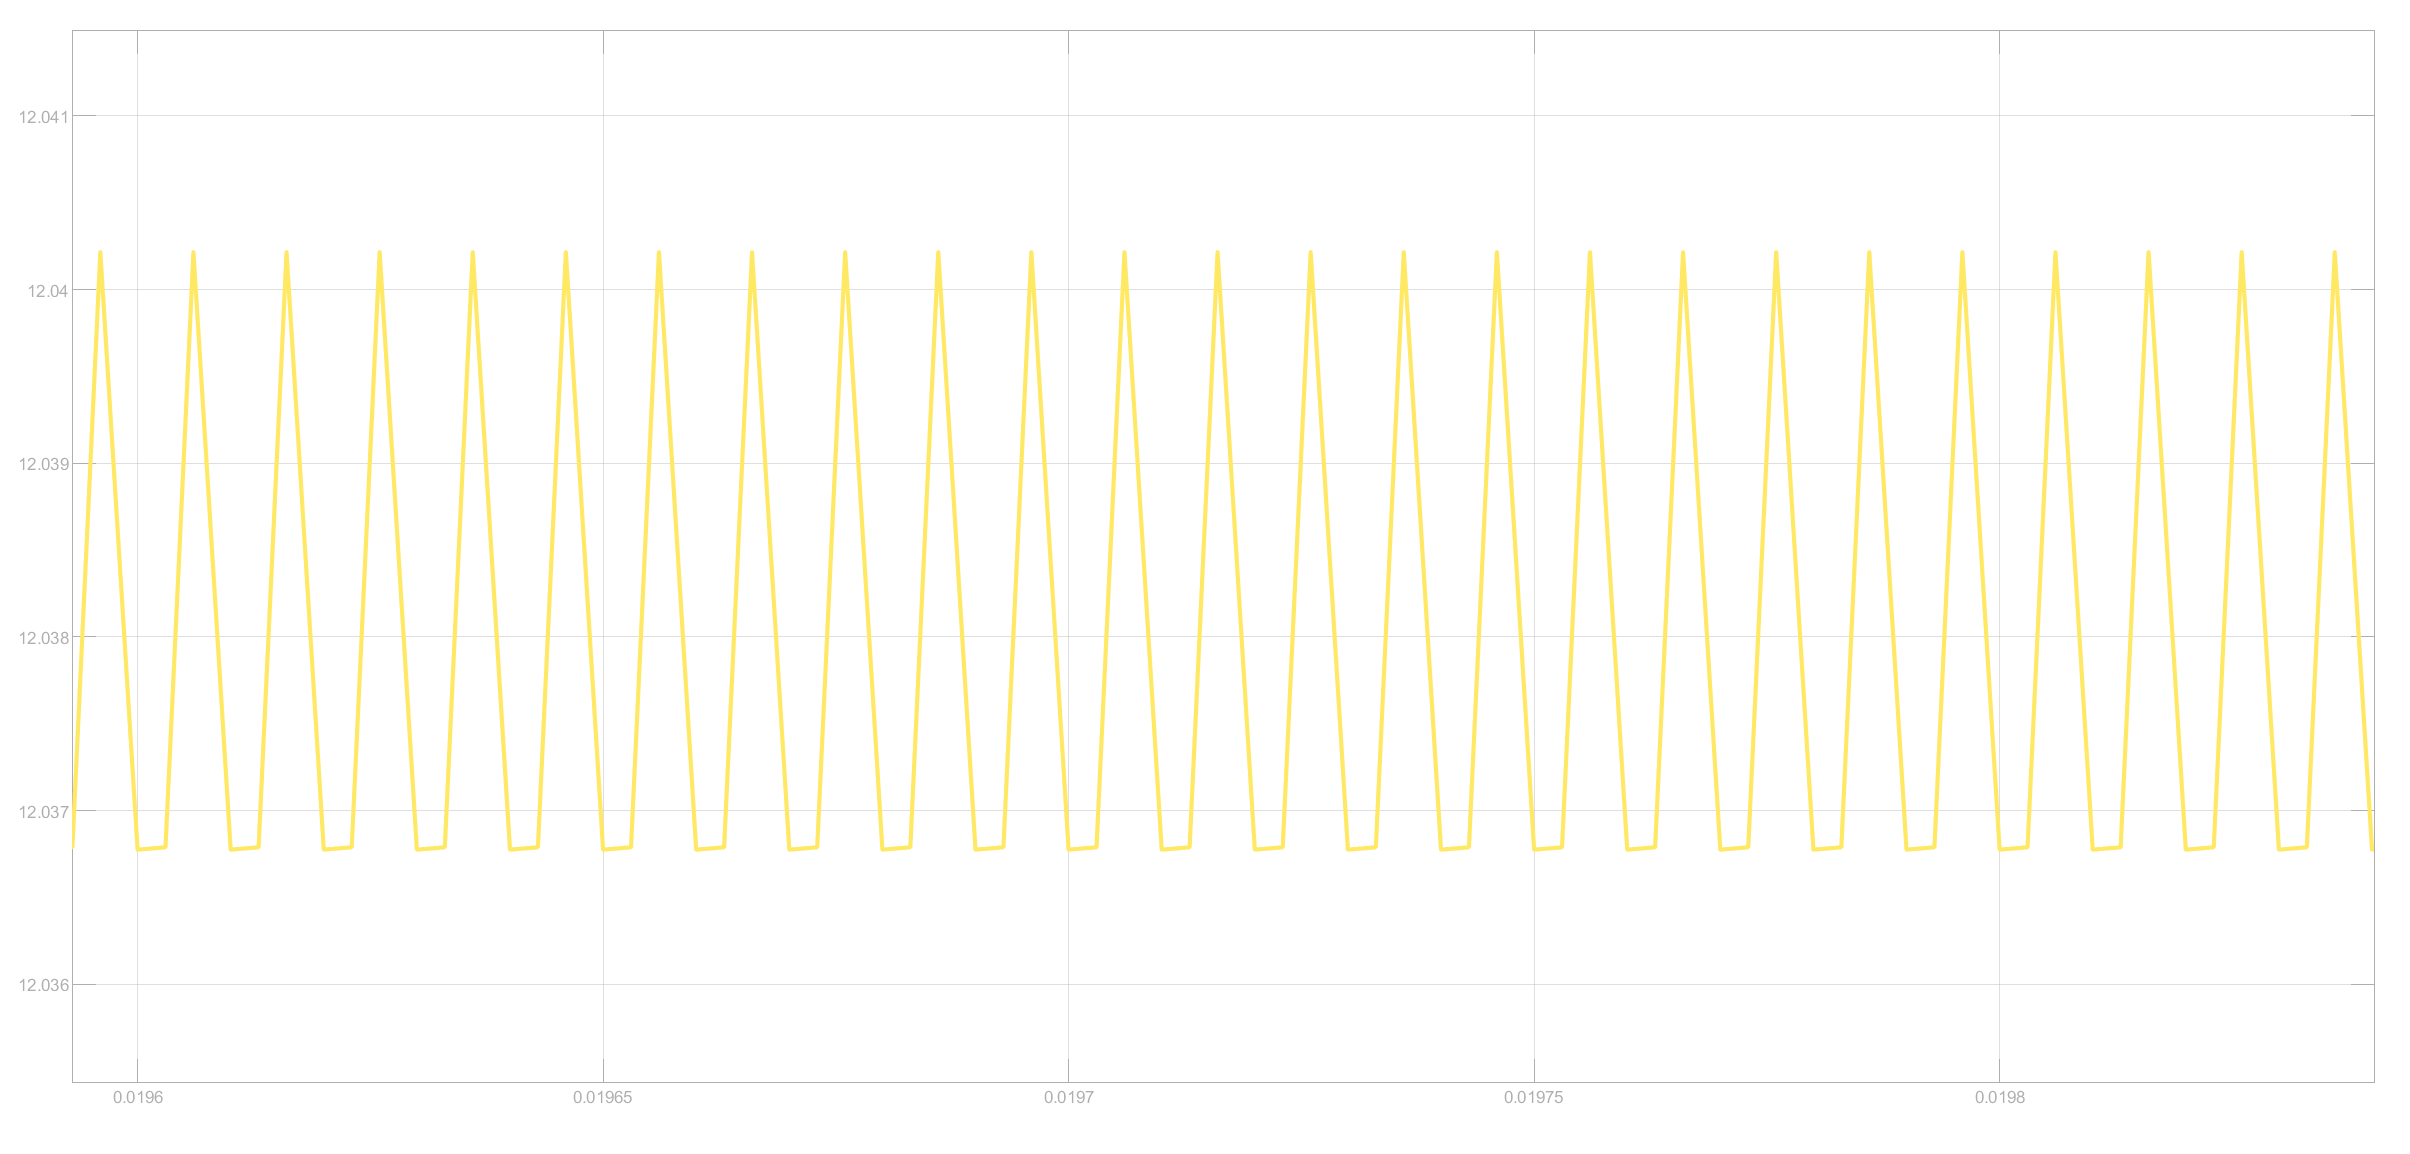
\includegraphics[width=0.8\textwidth]{image1.eps}
\caption{输入电压为42V时的电路仿真波形}
\end{figure}

由信号统计可知，输出电压纹波为$3.442mV$，双电平测量振幅为$3.407mV$，符合设计要求。
\newpage
\begin{figure}[htbp]
\centering
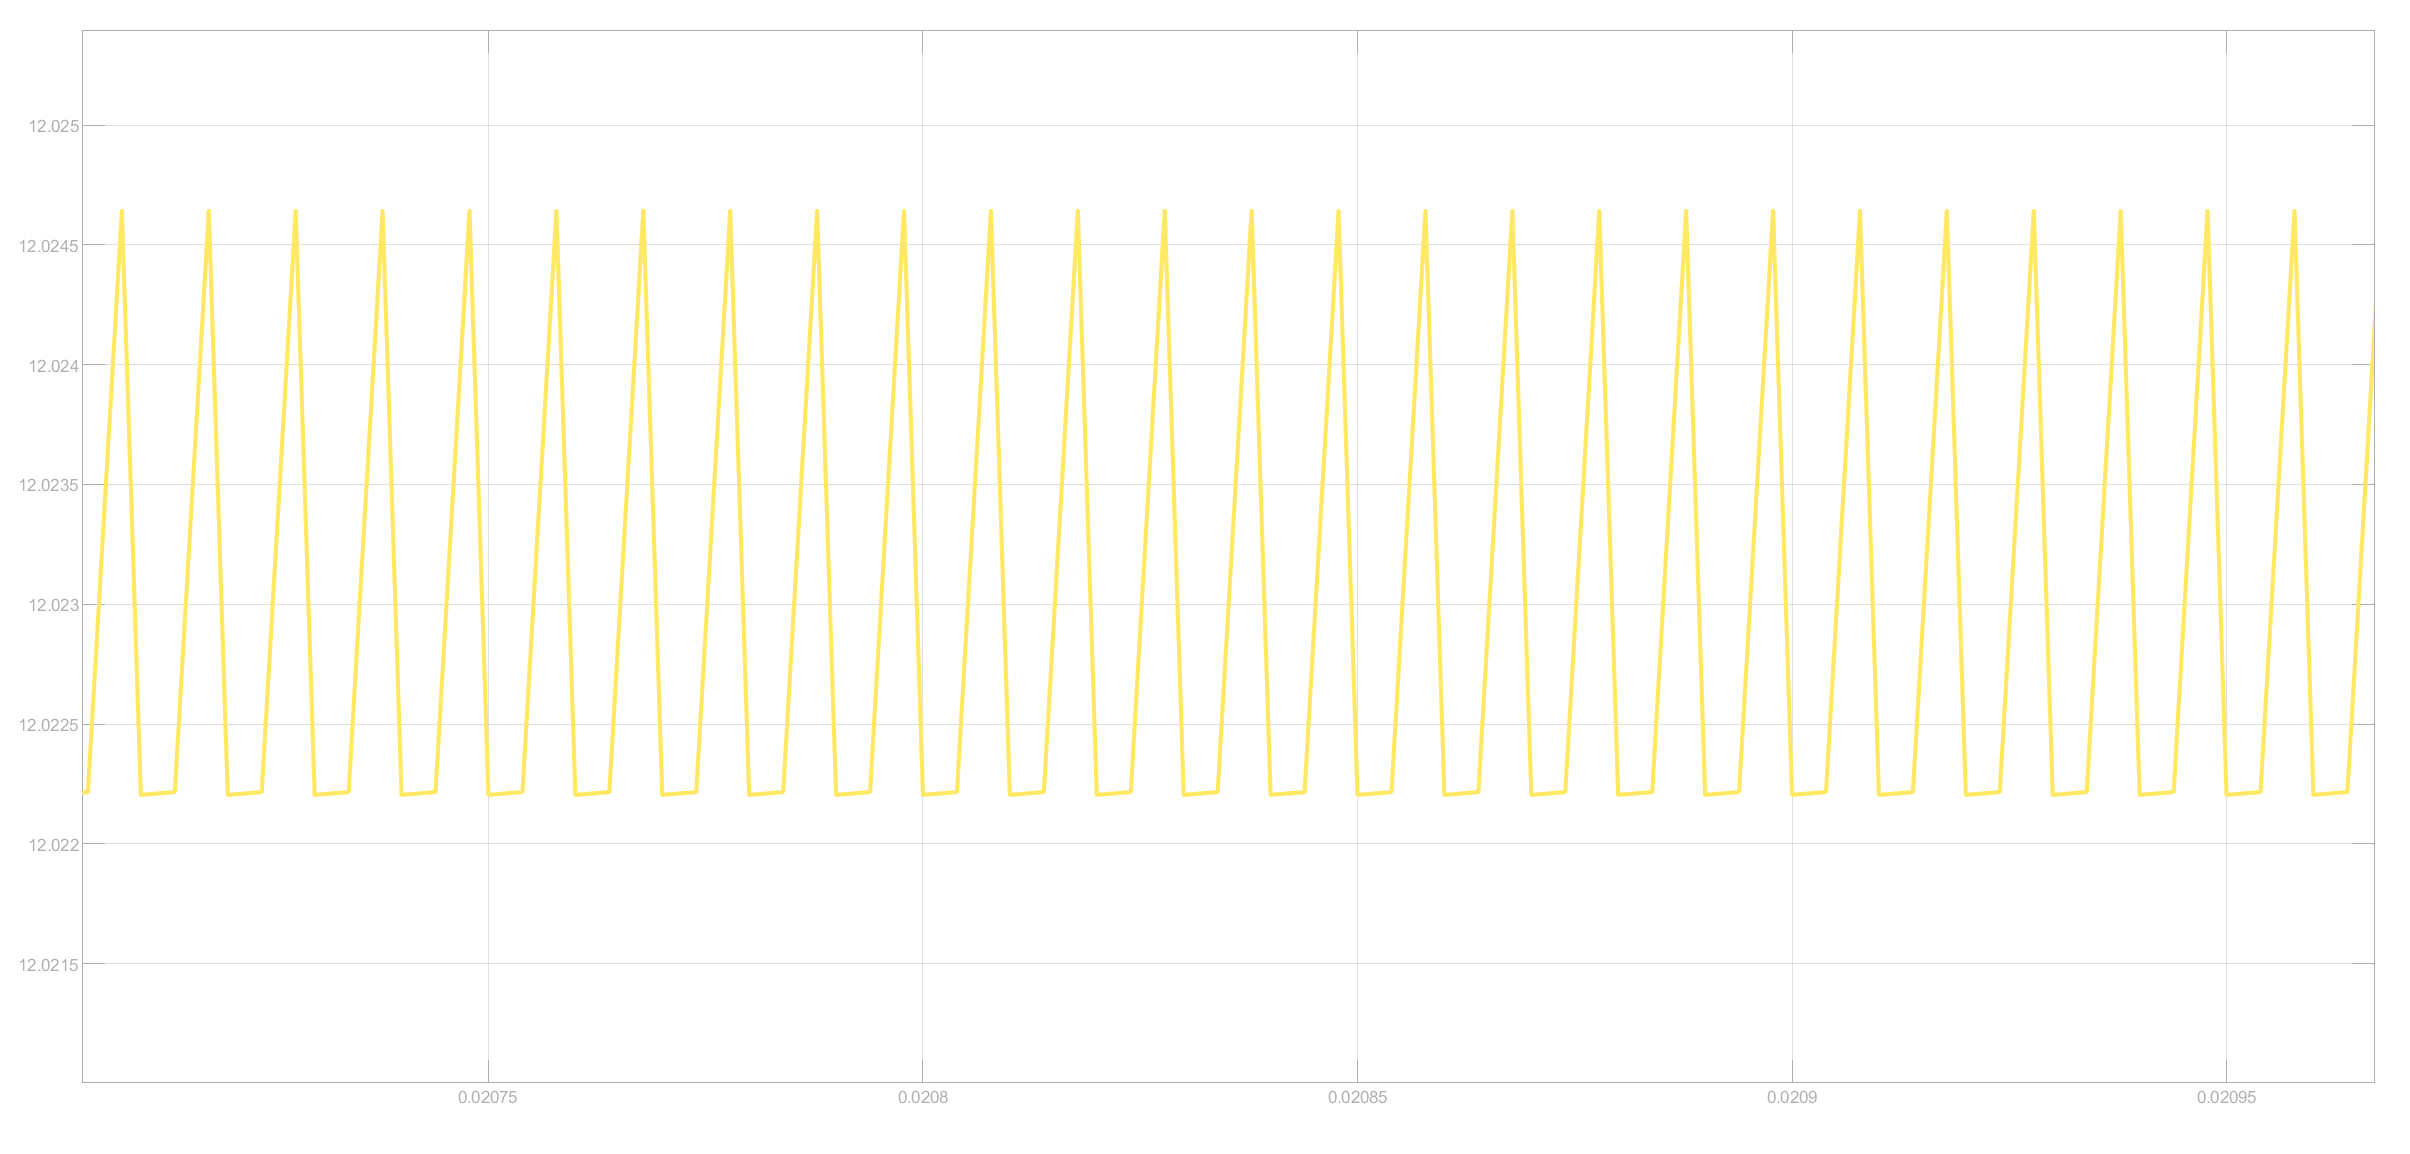
\includegraphics[width=0.8\textwidth]{image2.eps}
\caption{输入电压为32V时的电路仿真波形}
\end{figure}

由信号统计可知，输出电压纹波为$2.439mV$，双电平测量振幅为$2.415mV$，符合设计要求。
\begin{figure}[htbp]
\centering
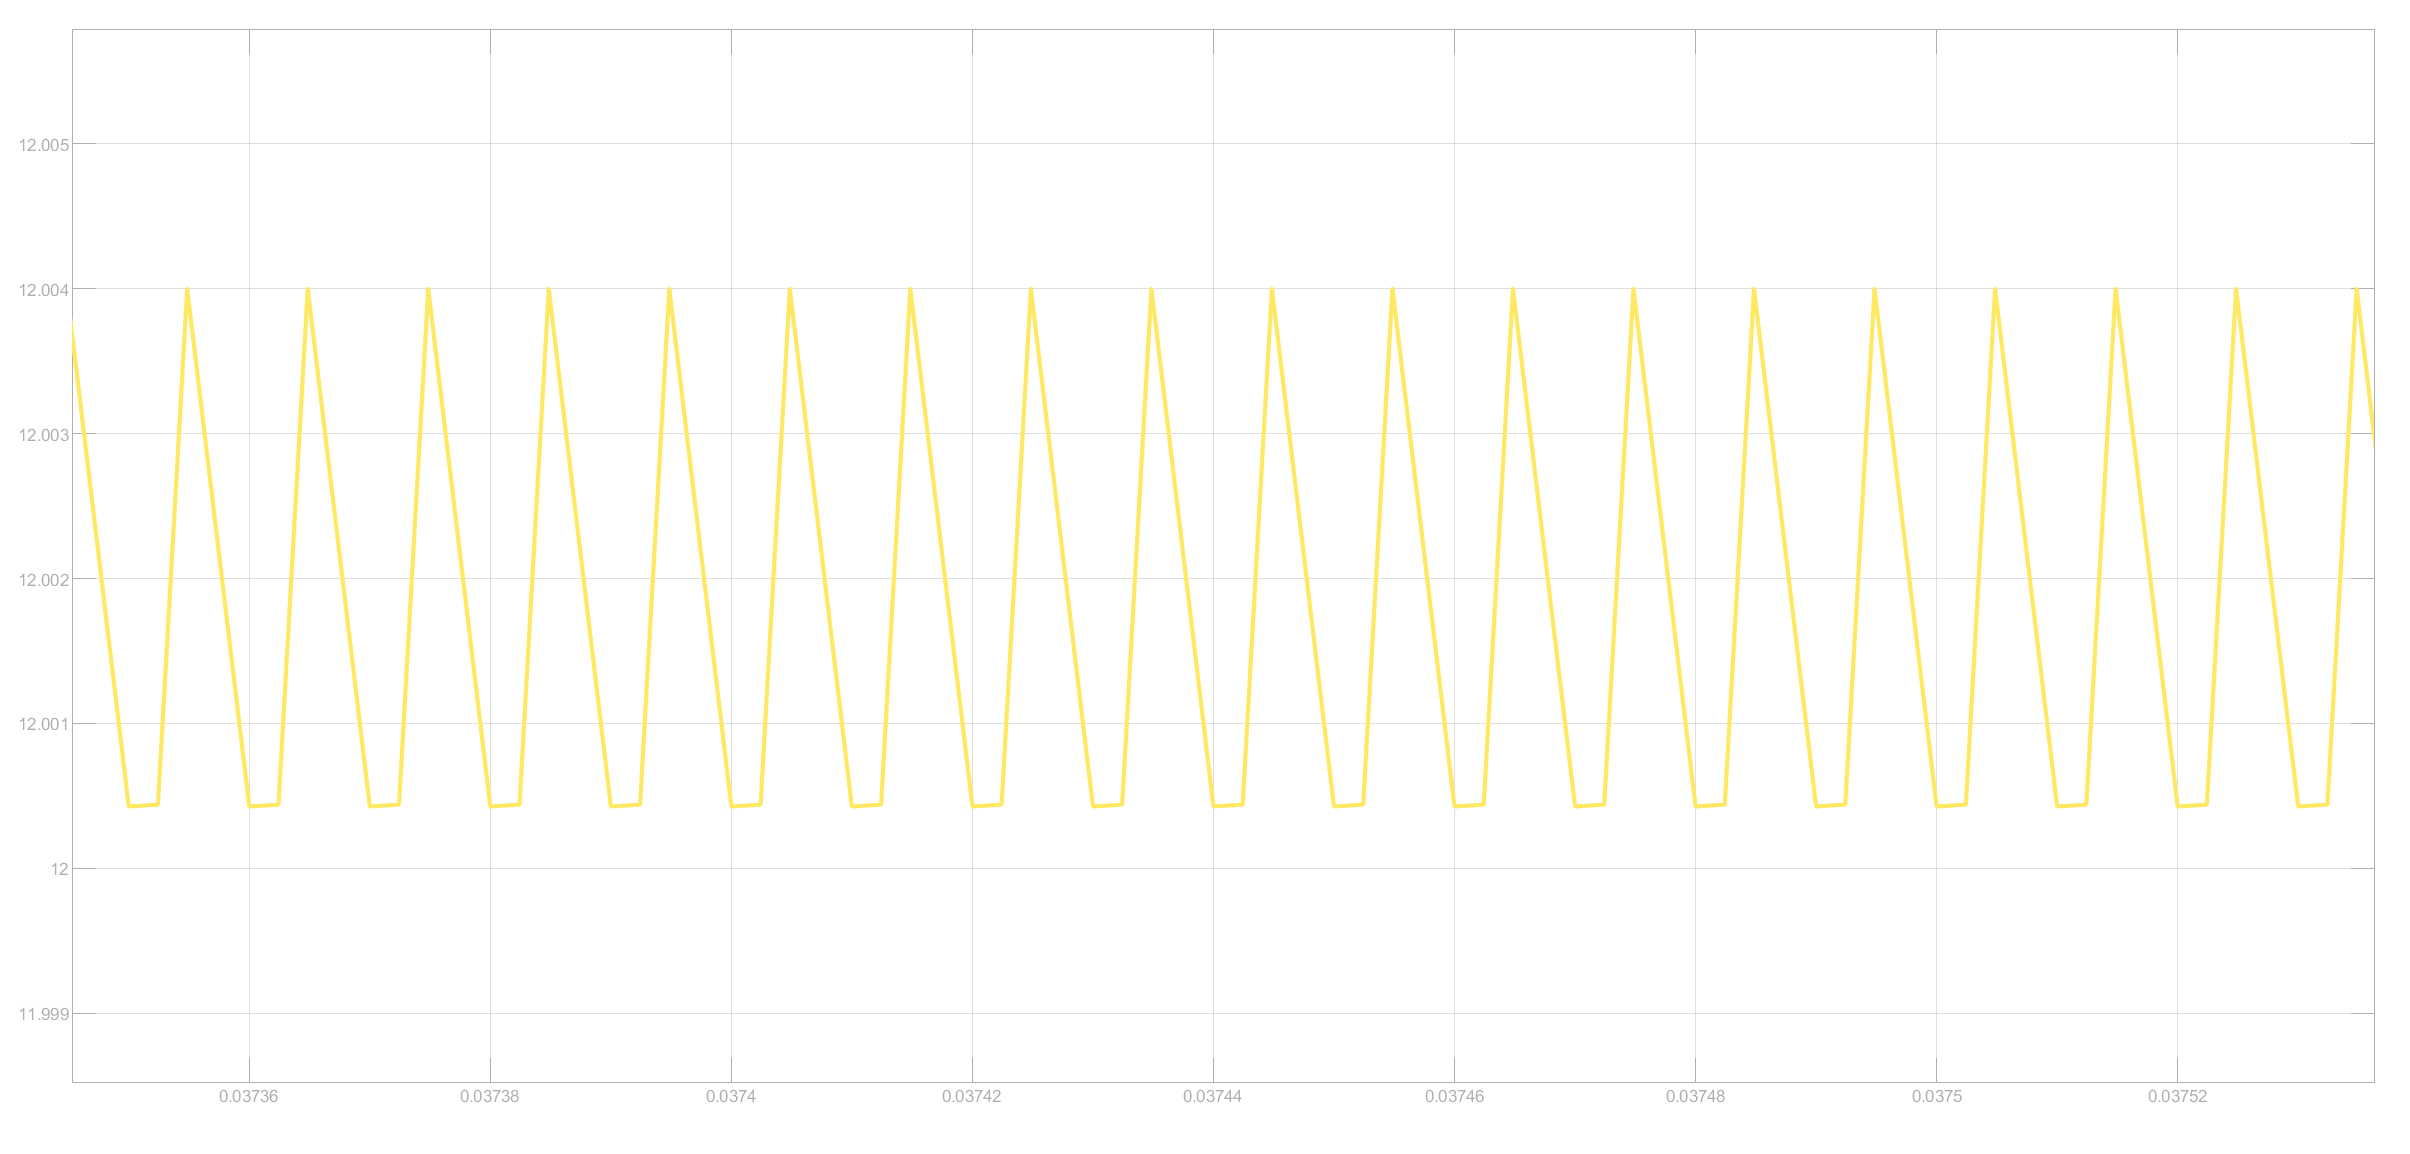
\includegraphics[width=0.8\textwidth]{image3.eps}
\caption{输入电压为52V时的电路仿真波形}
\end{figure}

由信号统计可知，输出电压纹波为$3.573mV$，双电平测量振幅为$3.538mV$，符合设计要求。

\section{ Buck 电路的 fuzzy 设计与仿真}
\subsection{设计框图}
\begin{figure}[htbp]
\centering
\includegraphics[width=0.8\textwidth]{1.png}
\caption{Buck 电路的 fuzzy 控制器设计框图}
\end{figure}
其中：Vref为参考电压，是一个常数：e为模糊控制器的输入误差：d/dt为输入误差的变化率，$K_e$和$K_{ec}$为量化因子，$K_u$为比例因子，C为反馈输出信号。
\subsection{设计过程}
（1）确定模糊控制器的输入和输出参数的确定

本次模糊控制系统为二输入-一输出，$K_e$、$K_{ec}$和$K_u$变量的模糊集论域都选择为$[-1,+1]$,隶属度函数采用常用的三角形隶属度函数。对于输入误差E,
其物理论域为$[-12,+12]$,所以$K_e$初步设定为$\tfrac{1}{12}$,对于误差变化率，考虑实际情况，当误差变化时，其变化一般比较大，假定为变化率为$[-100,+100]$，则$K_{ec}$可以初步设置为$100$:产生PWM的三角波幅值取为$1V$,则$K_u$取为1。

（2）Fuzzy Logic Designer设计模糊控制器

利用MATLAB中的Fuzzy Logic Designer工具箱设计模糊控制器，
分别对输入误差E和误差变化率EC以及输出控制量U进行模糊化处理，
输入范围是-1到1;输出范围是-1到1;且对它们均设置7个隶屈度函数。
定义各自的隶属函数和模糊规则表。

模糊控制规则表如下所示：
\begin{table}[h]
\centering
\begin{tabular}{c|ccccccc}
\diagbox{E}{EC} & NB & NM & NS & ZE & PS & PM & PB \\
\hline
NB & NB & NB & NB & NB & NM & NS & ZE \\
NM & NB & NB & NM & NS & NB & ZE & PS \\
NS & NB & NB & NM & NS & ZE & PS & PM \\
ZE & NB & NM & NS & ZE & PS & PM & PB \\
PS & NM & NS & ZE & PS & PM & PB & PB \\
PM & NS & ZE & PS & PM & PB & PB & PB \\
PB & ZE & PS & PM & PB & PB & PB & PB \\
\end{tabular}
\caption{模糊控制规则表}
\end{table}

隶属函数如下图所示：
\newpage
\begin{figure}[h]
\centering 
\includegraphics[width=0.8\textwidth]{2.png}
\caption{输入误差E的隶属函数}
\end{figure}
\newpage
\begin{figure}[h]
\centering  
\includegraphics[width=0.8\textwidth]{3.png}
\caption{误差变化率EC的隶属函数}
\end{figure}
\newpage
\begin{figure}[h]
\centering  
\includegraphics[width=0.8\textwidth]{4.png}
\caption{输出电压U的隶属函数}
\end{figure}
\newpage
控制曲面如下图所示：
\begin{figure}[h]
\centering  
\includegraphics[width=0.8\textwidth]{5.png}
\caption{模糊控制器的控制曲面}
\end{figure}
\newpage

（3）搭建Simulink仿真模型

需要说明的是：在仿真过程中，100\%负载时，负载电阻取为$R=\tfrac{V_{out}}{I_{out,max}}=\tfrac{12V}{2A}=6\Omega$;
10\%负载时，负载电阻取为$R=\tfrac{V_{out}}{I_{out,min}}=\tfrac{12V}{0.2A}=60\Omega$。

 Buck 电路的 fuzzy 控制器Simulink仿真模型如下图所示：

\begin{figure}[htbp]
\centering  
\includegraphics[width=0.8\textwidth]{6.png}
\caption{Buck 电路的 fuzzy 控制仿真模型}
\end{figure}
\newpage
仿真过程中主要调节了E和EC两路的量化因子，调节这两个数值，最终确定$K_e$为40,	$K_{ec}$为400, fuzzy控制的输出结果基本满足要求。

\textcircled{1}当输入电压为42V时

在稳态负载下仿真波形如下：
\begin{figure}[htbp]
\centering  
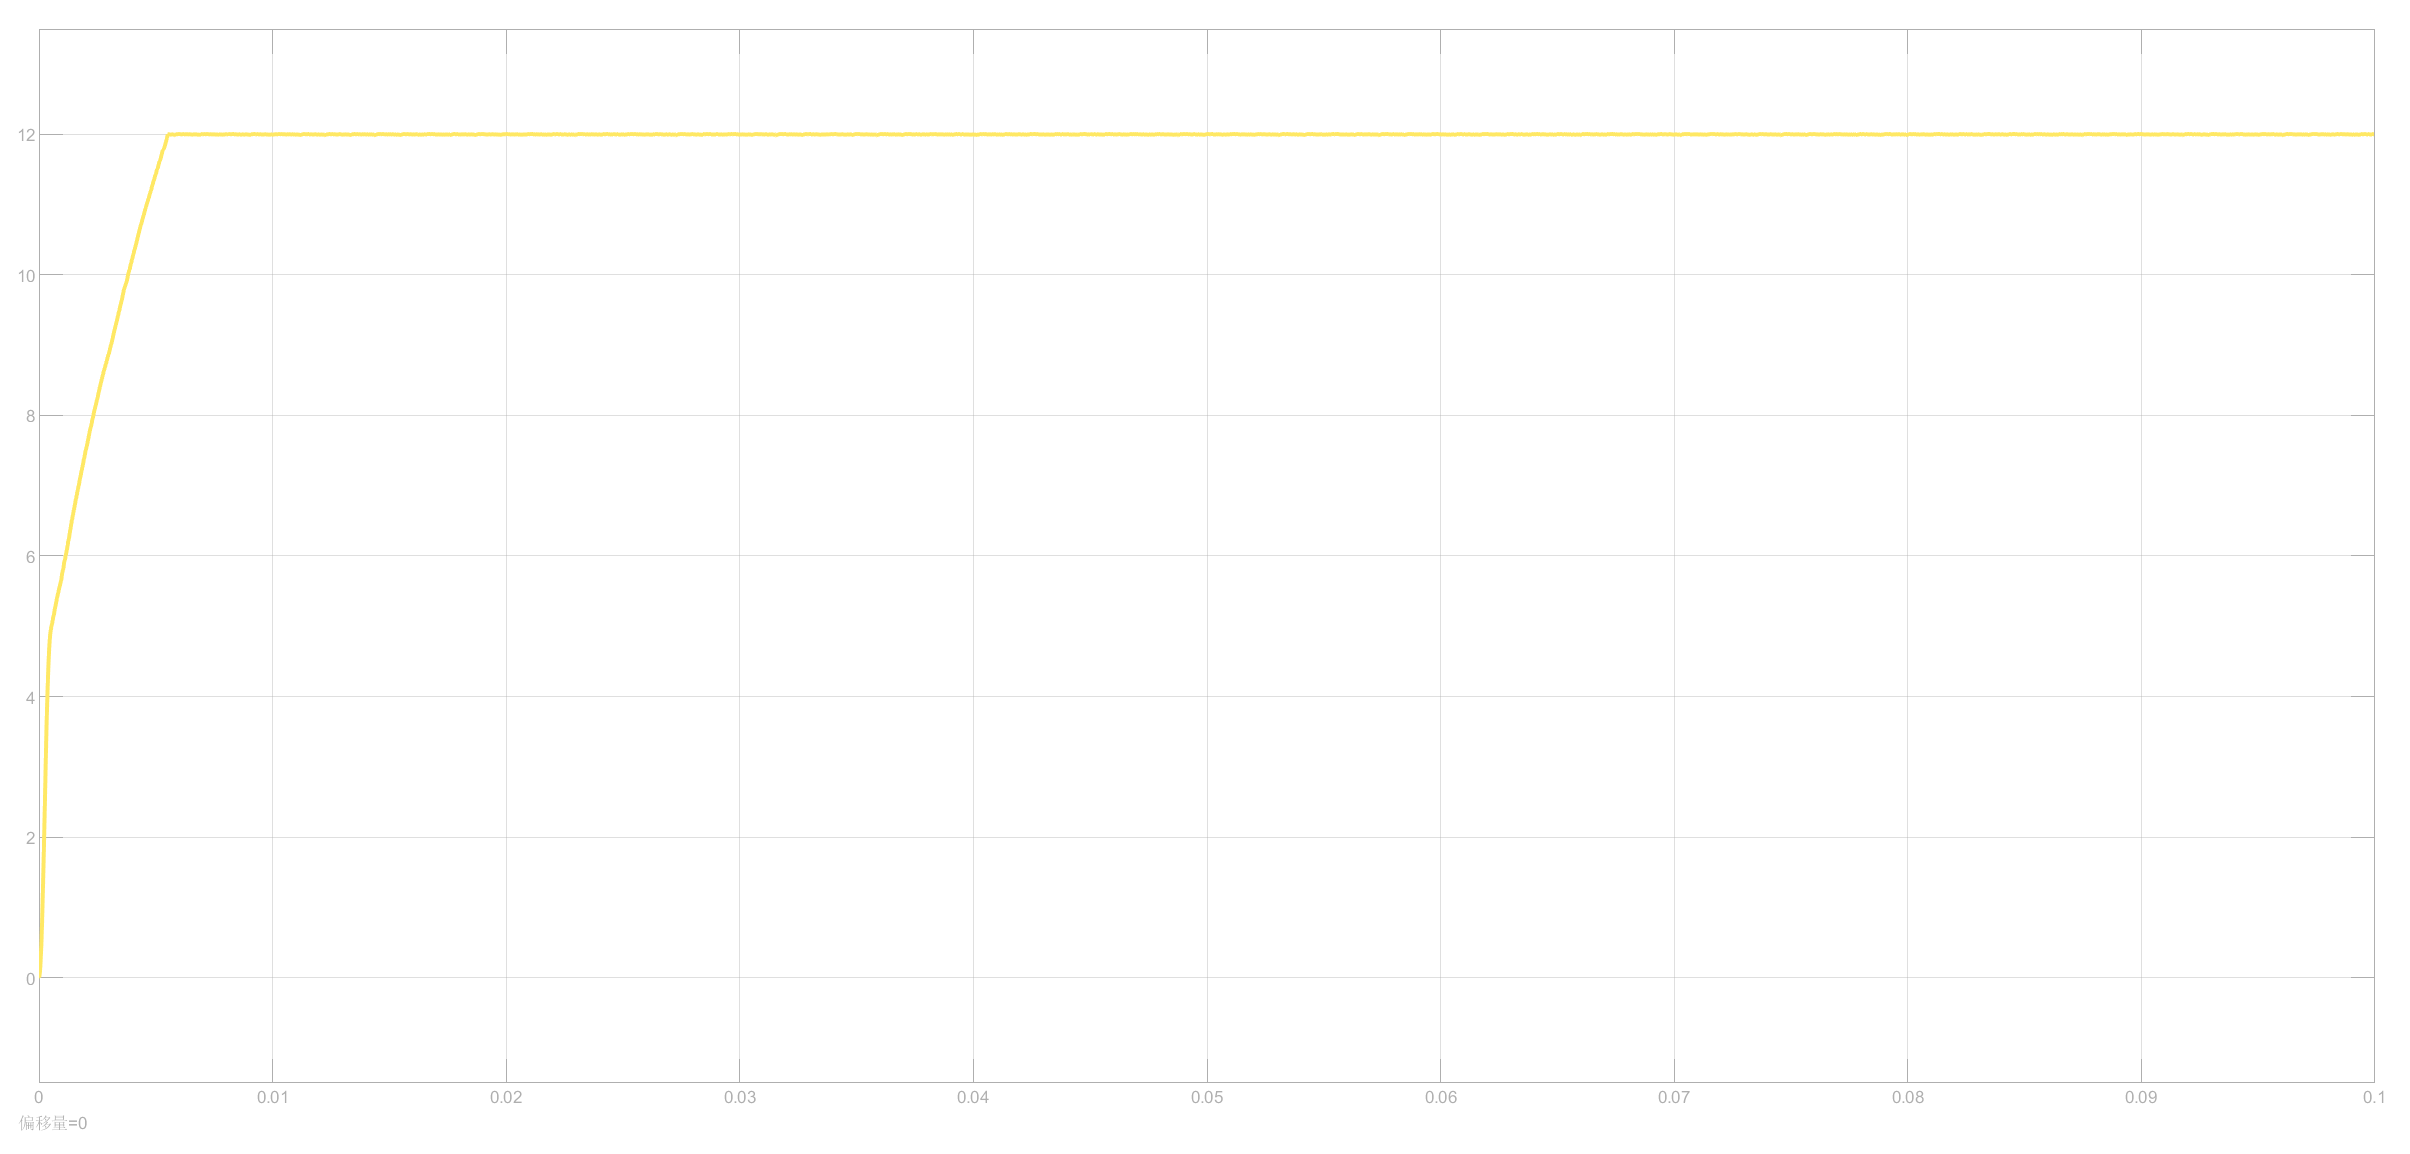
\includegraphics[width=0.8\textwidth]{image4.eps}
\caption{输入电压为42V，未加切载时，系统仿真结果}
\end{figure}

单独观察电压纹波：
\begin{figure}[h]
\centering  
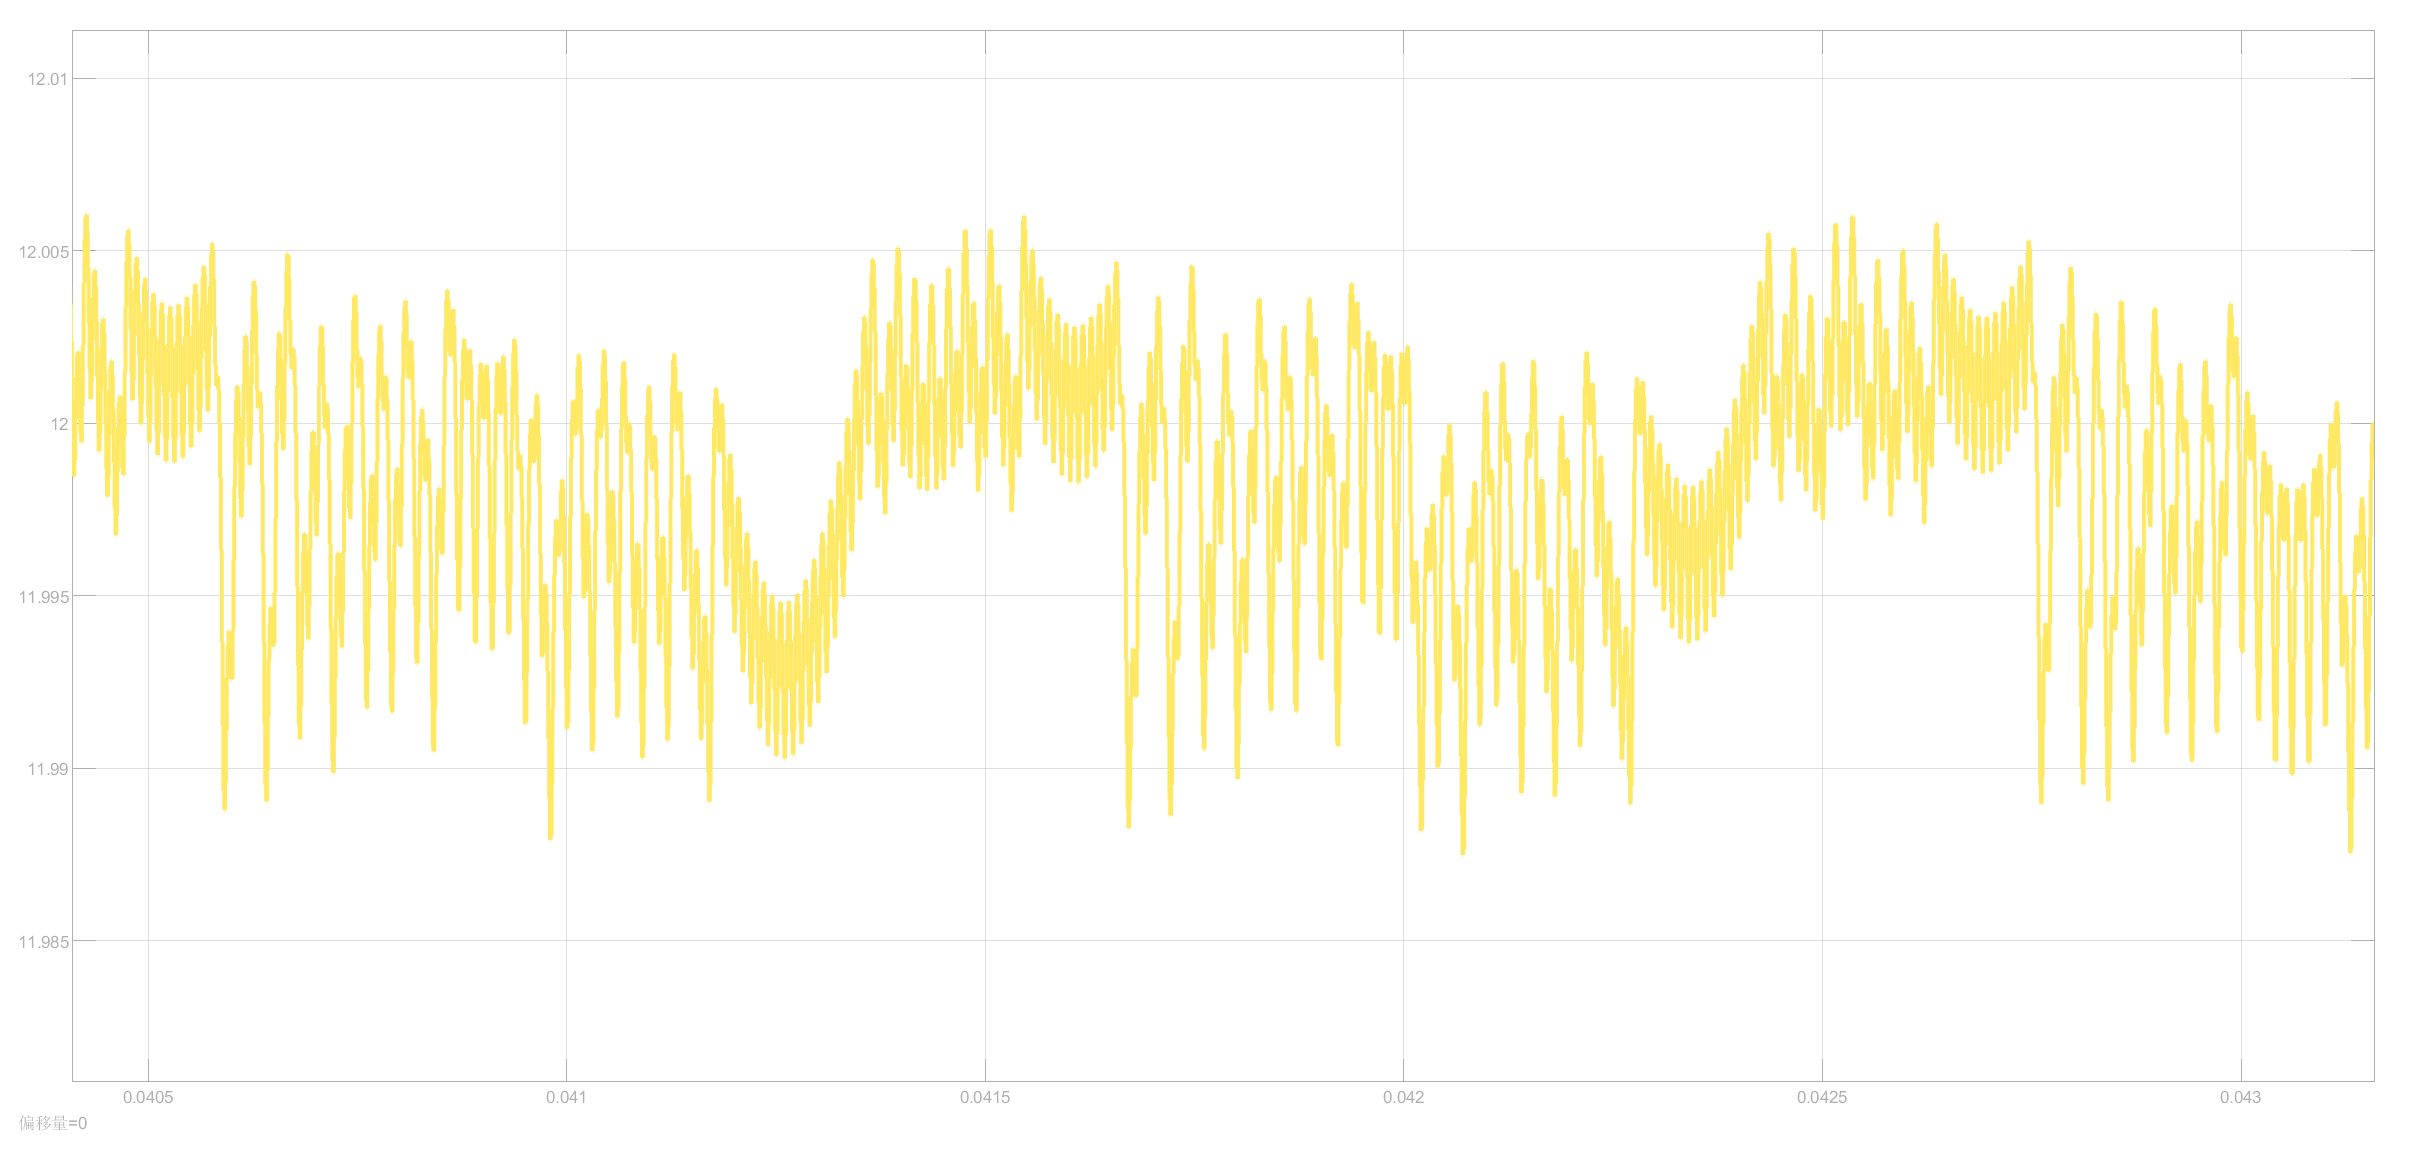
\includegraphics[width=0.8\textwidth]{image5.eps}
\caption{输出电压的纹波}
\end{figure}

由信号统计可知，输出电压纹波为$18.58mV$，双电平测量振幅为$3.902mV$。
\newpage
加入切载时，系统仿真结果如下：
\begin{figure}[htbp]
\centering  
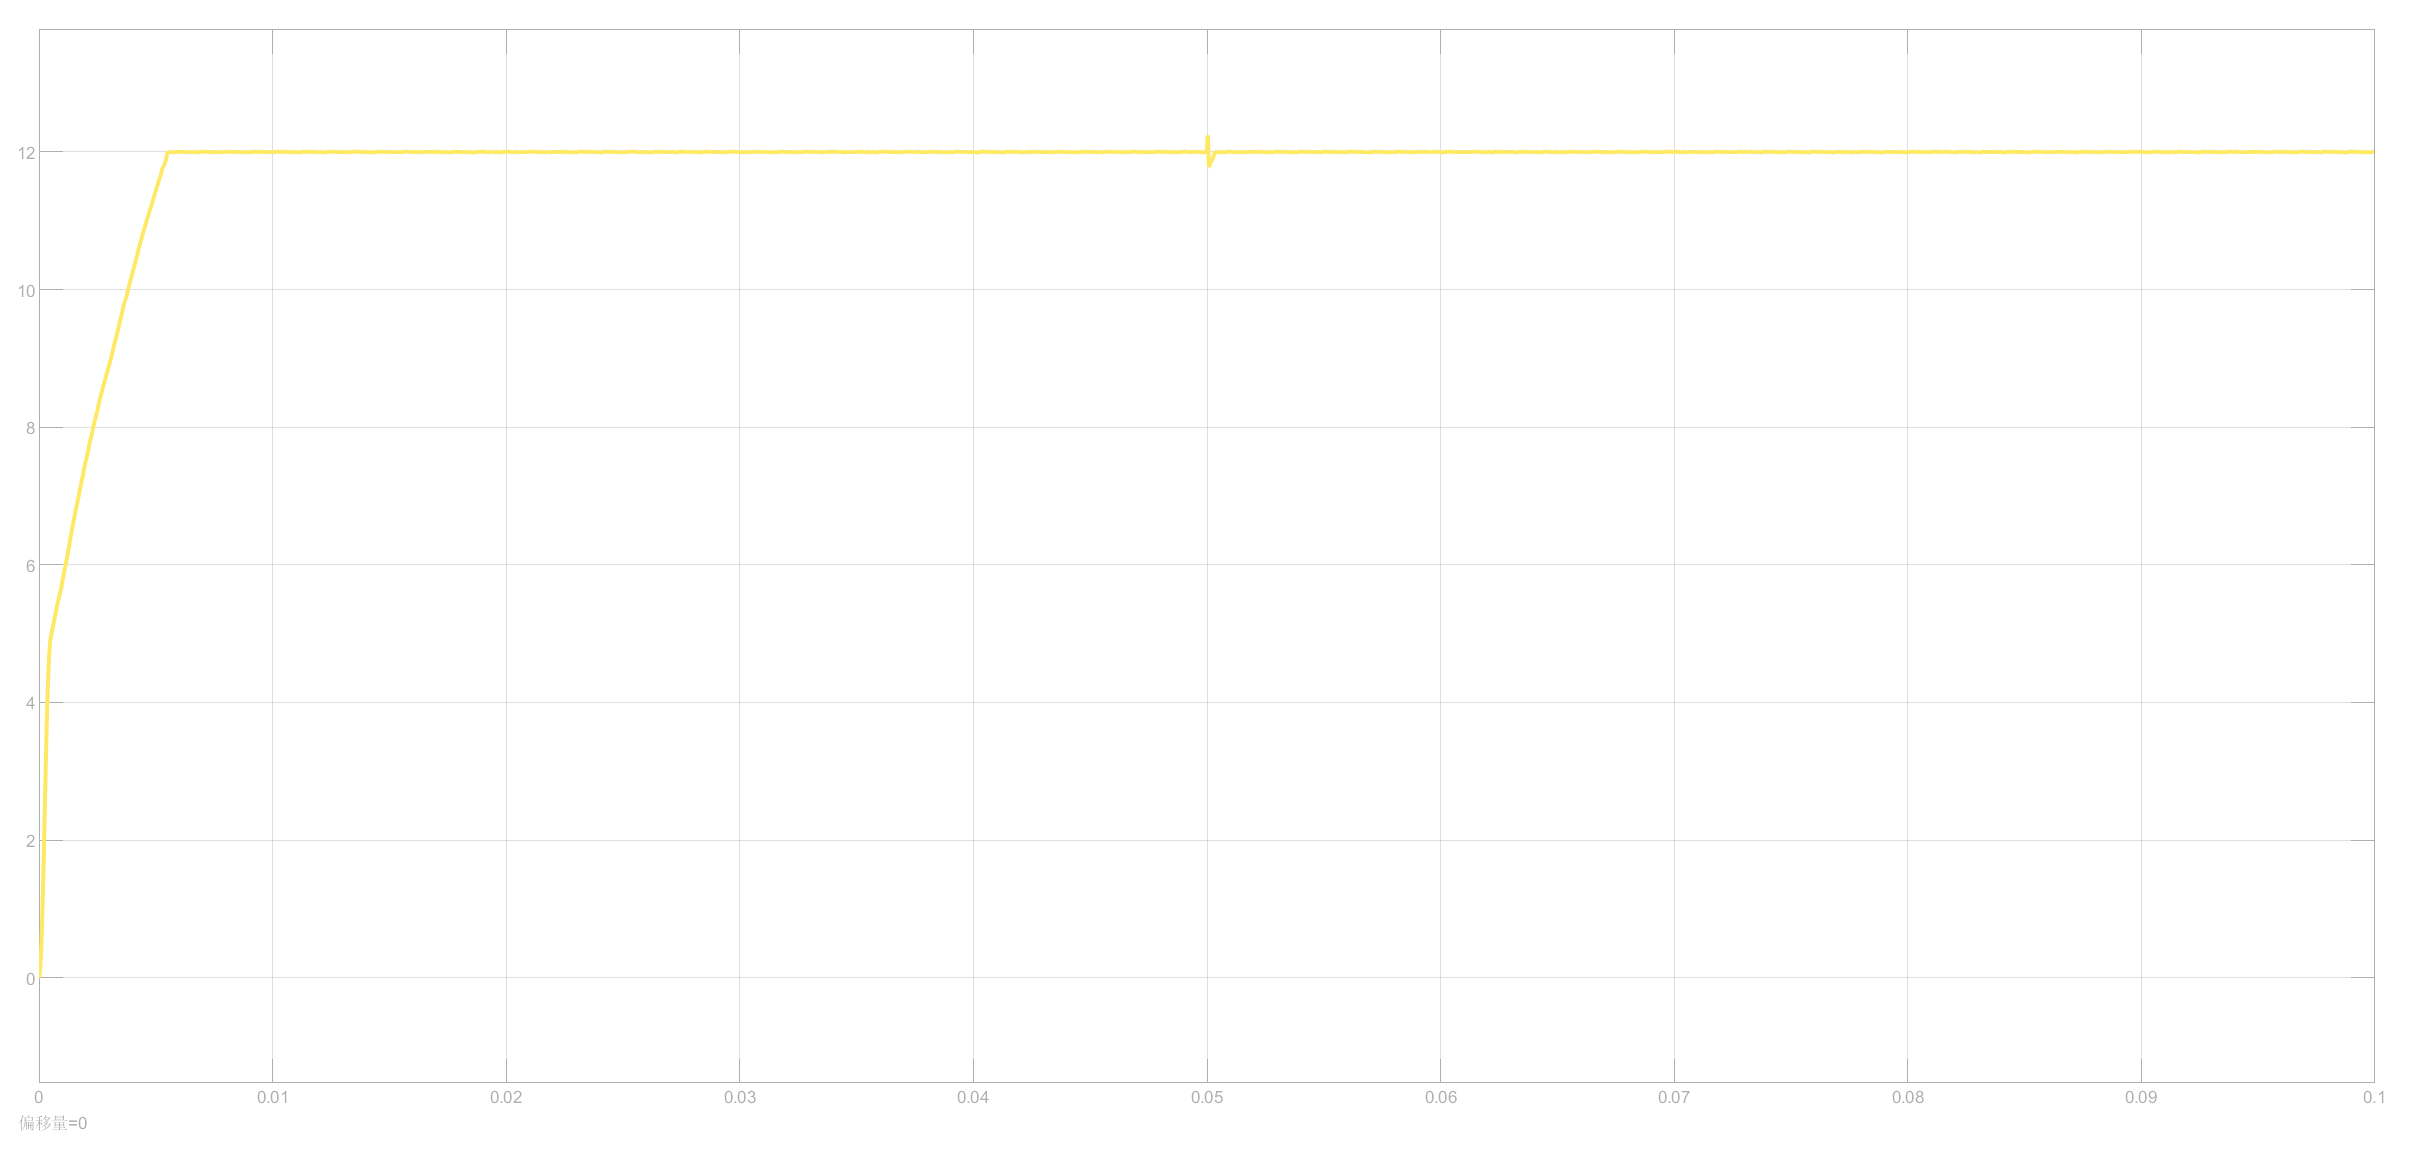
\includegraphics[width=0.8\textwidth]{image6.eps}
\caption{输入电压为42V，加入切载时，系统仿真结果}
\end{figure}

由信号统计可知，在$t=0.05s$处施加$10\%-100\%$的切载过程，输出电压超调量为$0.24V$，切载引起的电压跌落到$11.78V$,小于设计要求的$5\% \times 12V=0.6V$。

\textcircled{2}当输入电压为52V时

在稳态负载下仿真波形如下：
\begin{figure}[htbp]
\centering  
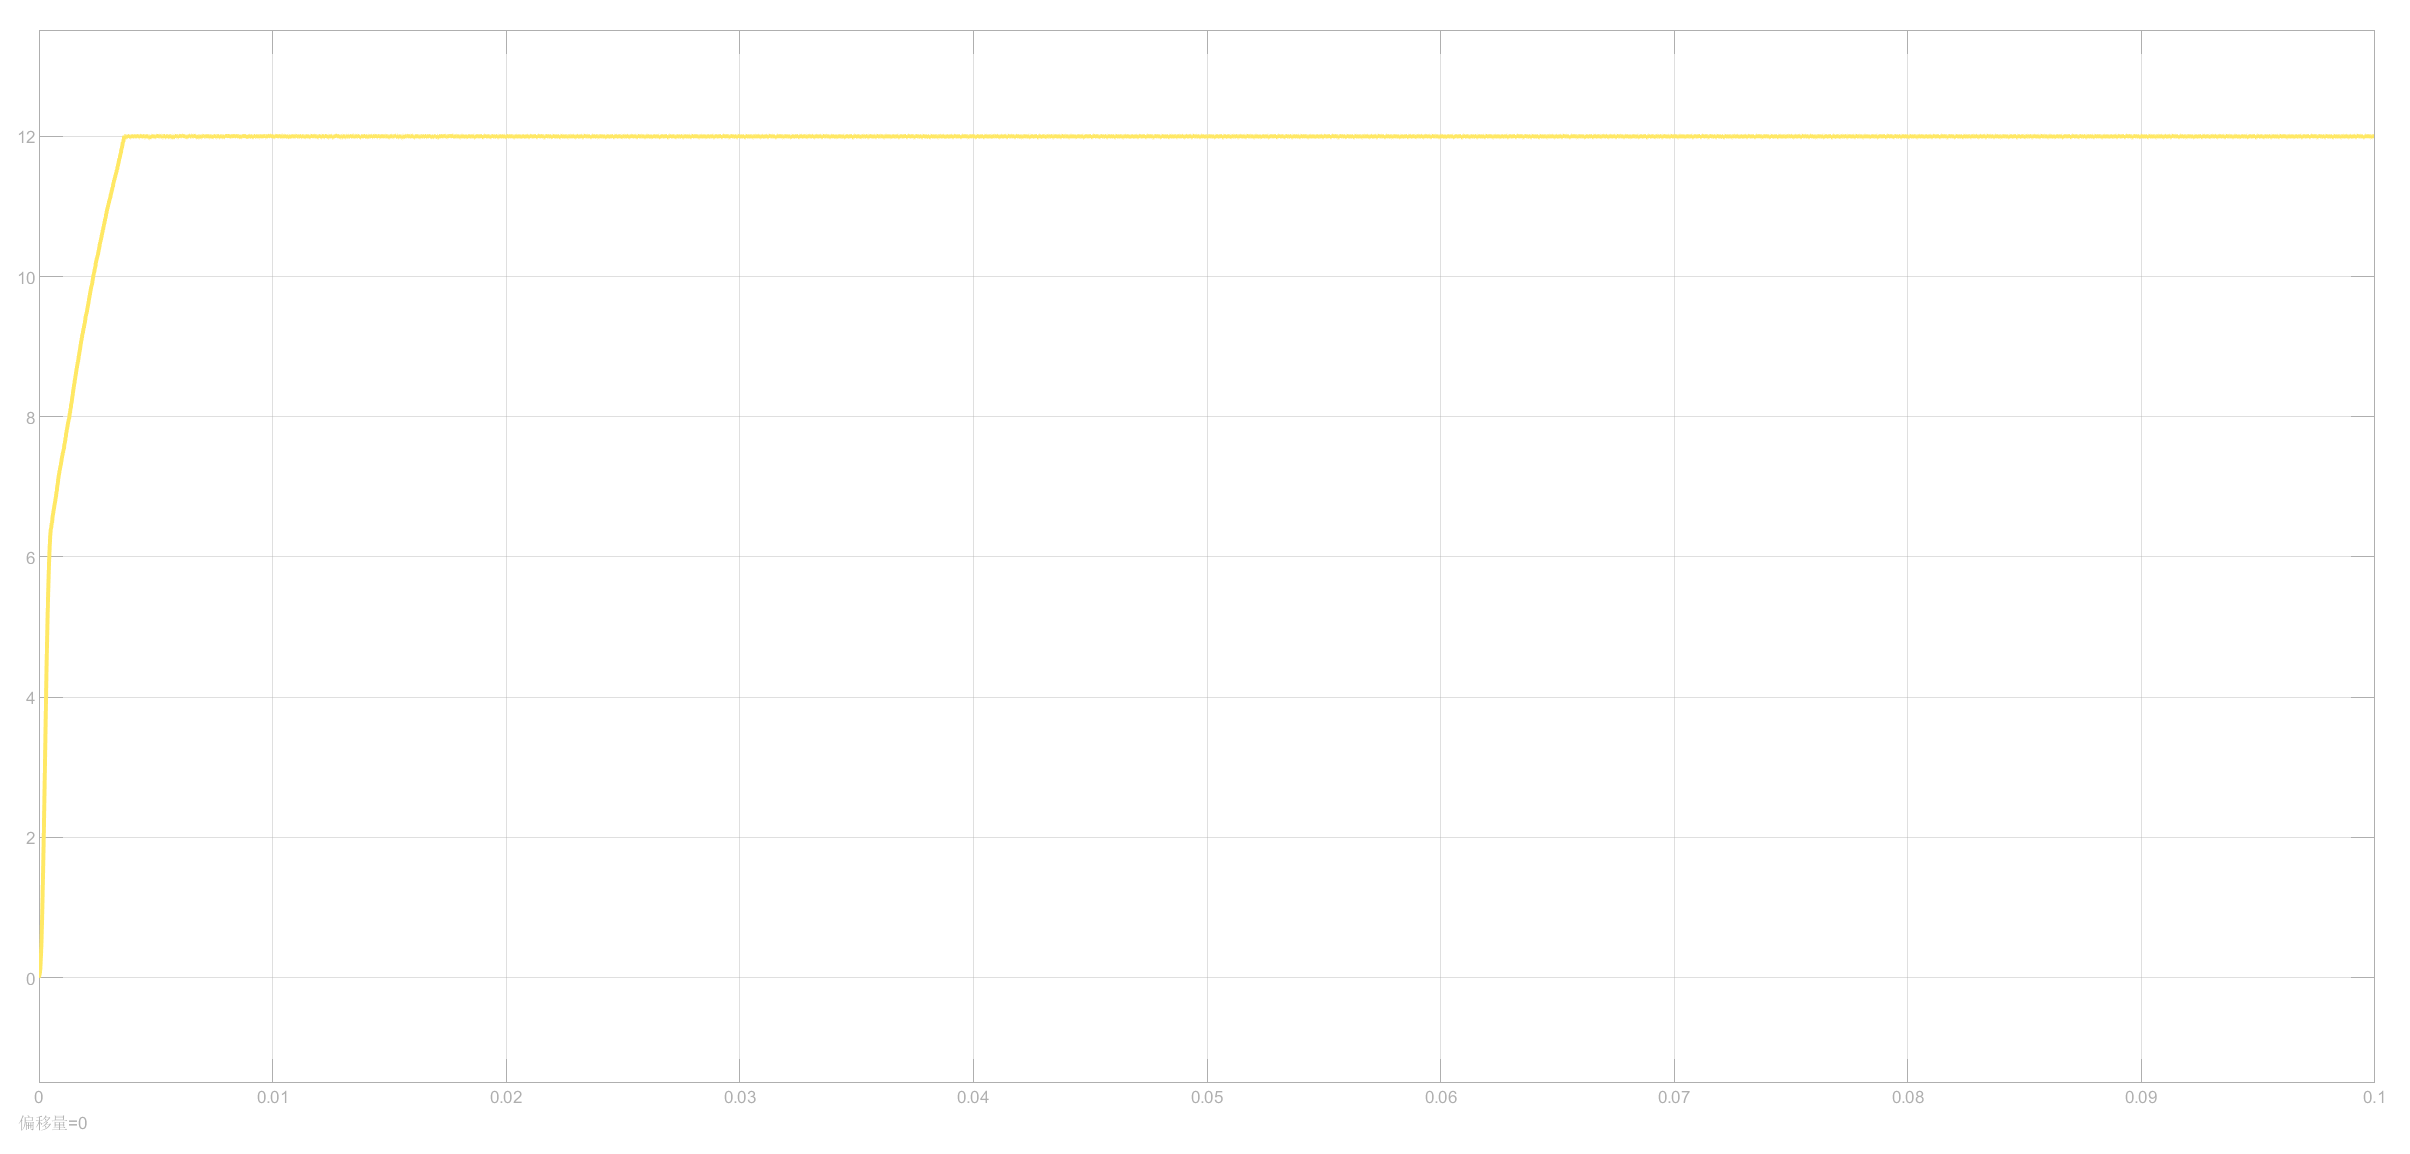
\includegraphics[width=0.8\textwidth]{image7.eps}
\caption{输入电压为52V，未加切载时，系统仿真结果}
\end{figure}

单独观察电压纹波：
\begin{figure}[h]
\centering  
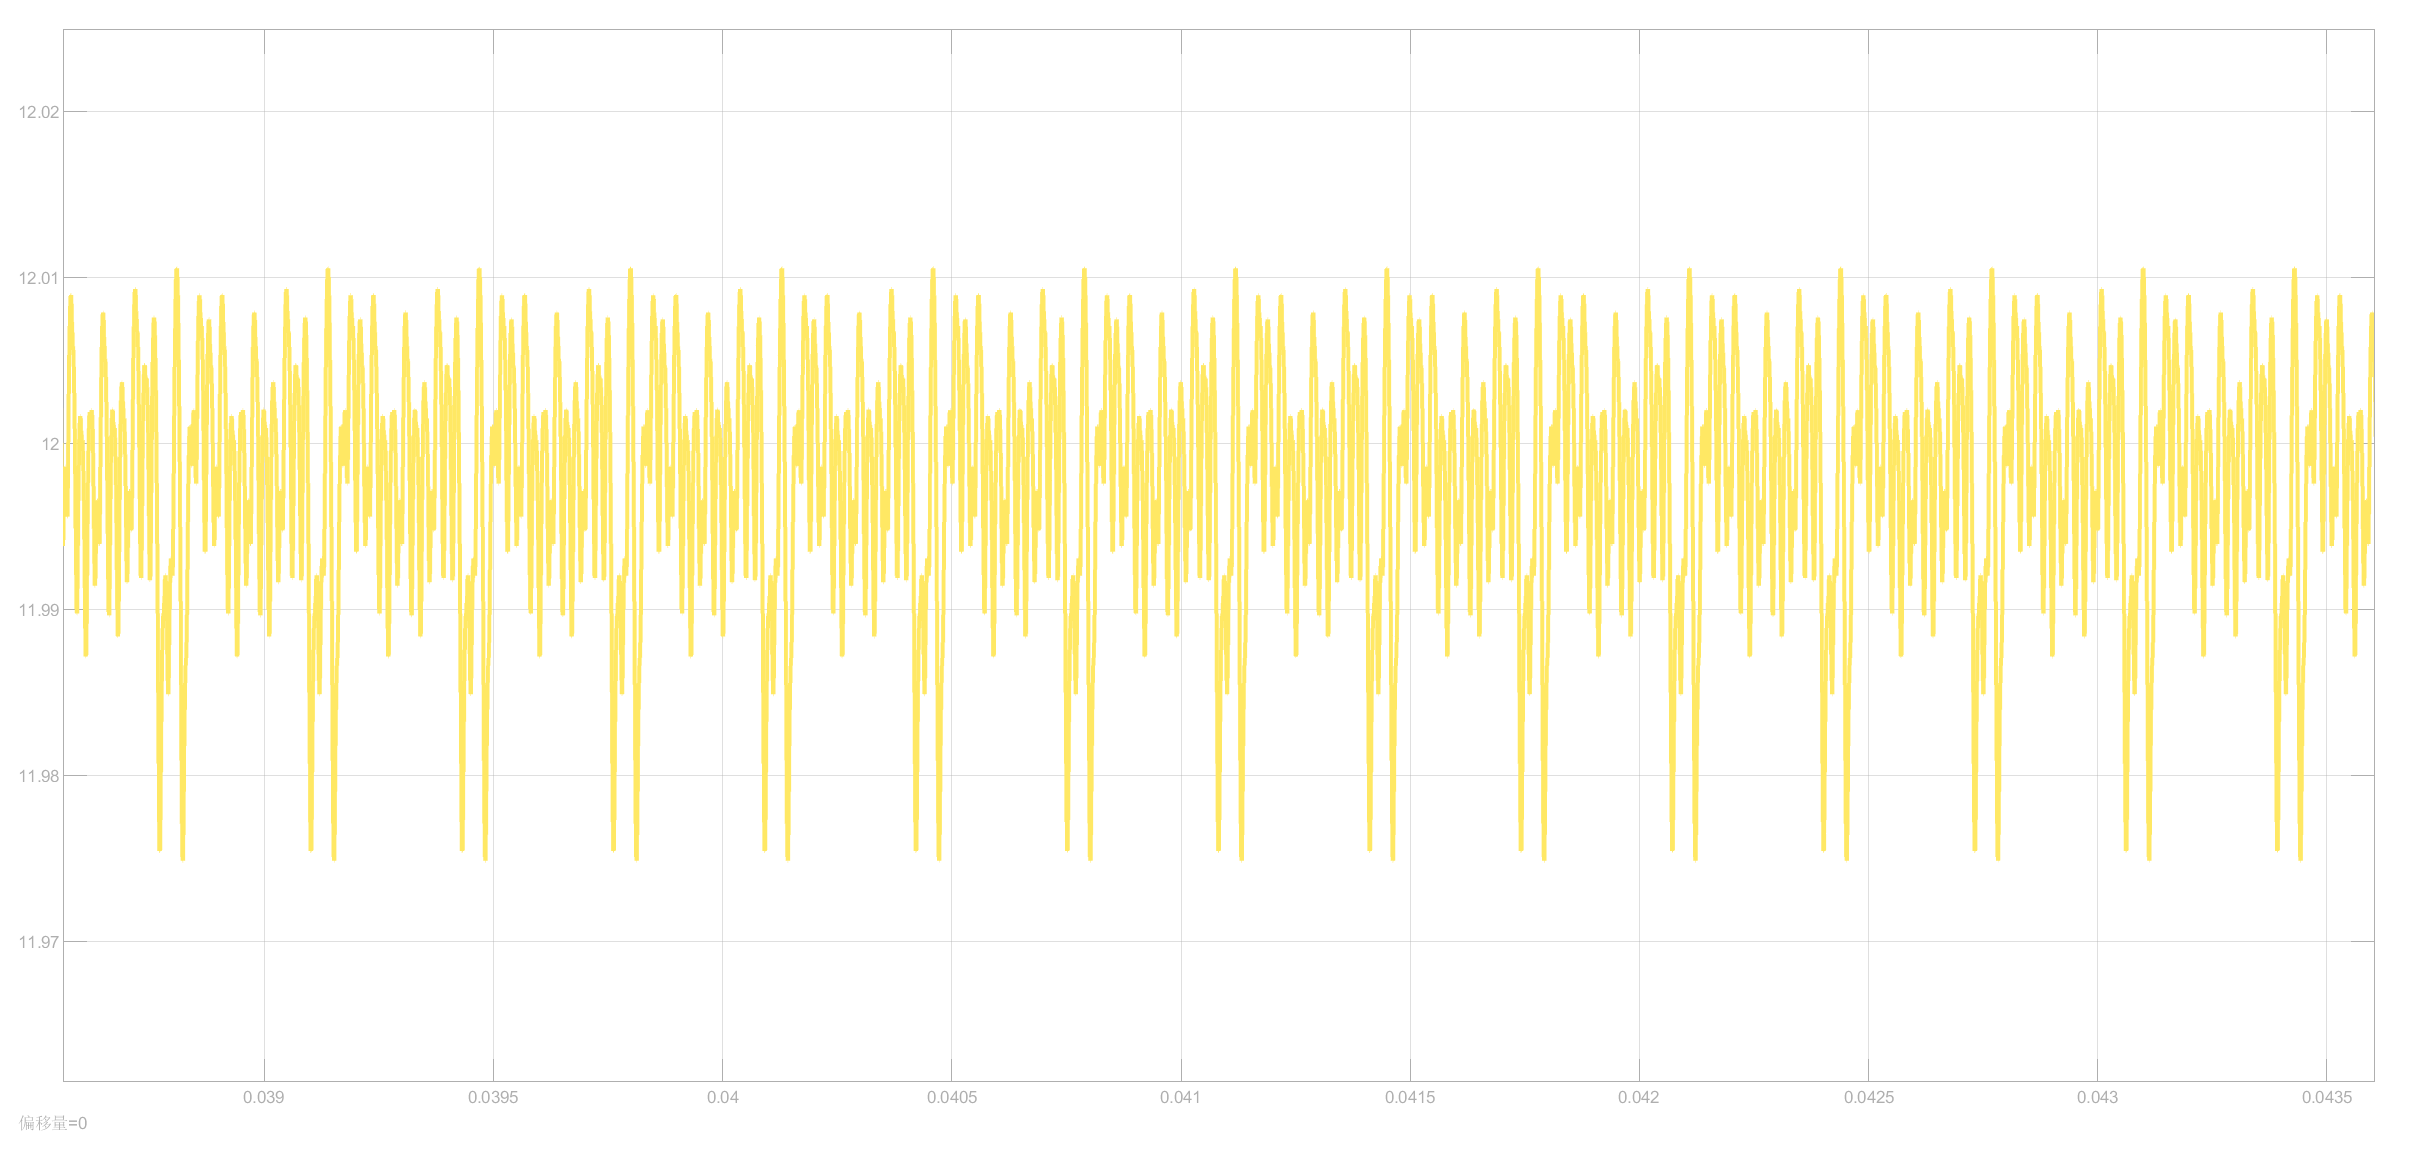
\includegraphics[width=0.8\textwidth]{image8.eps}
\caption{输出电压的纹波}
\end{figure}
\newpage
由信号统计可知，输出电压纹波为$35.69mV$，双电平测量振幅为$9.635mV$。

加入切载时，系统仿真结果如下：
\begin{figure}[htbp]
\centering  
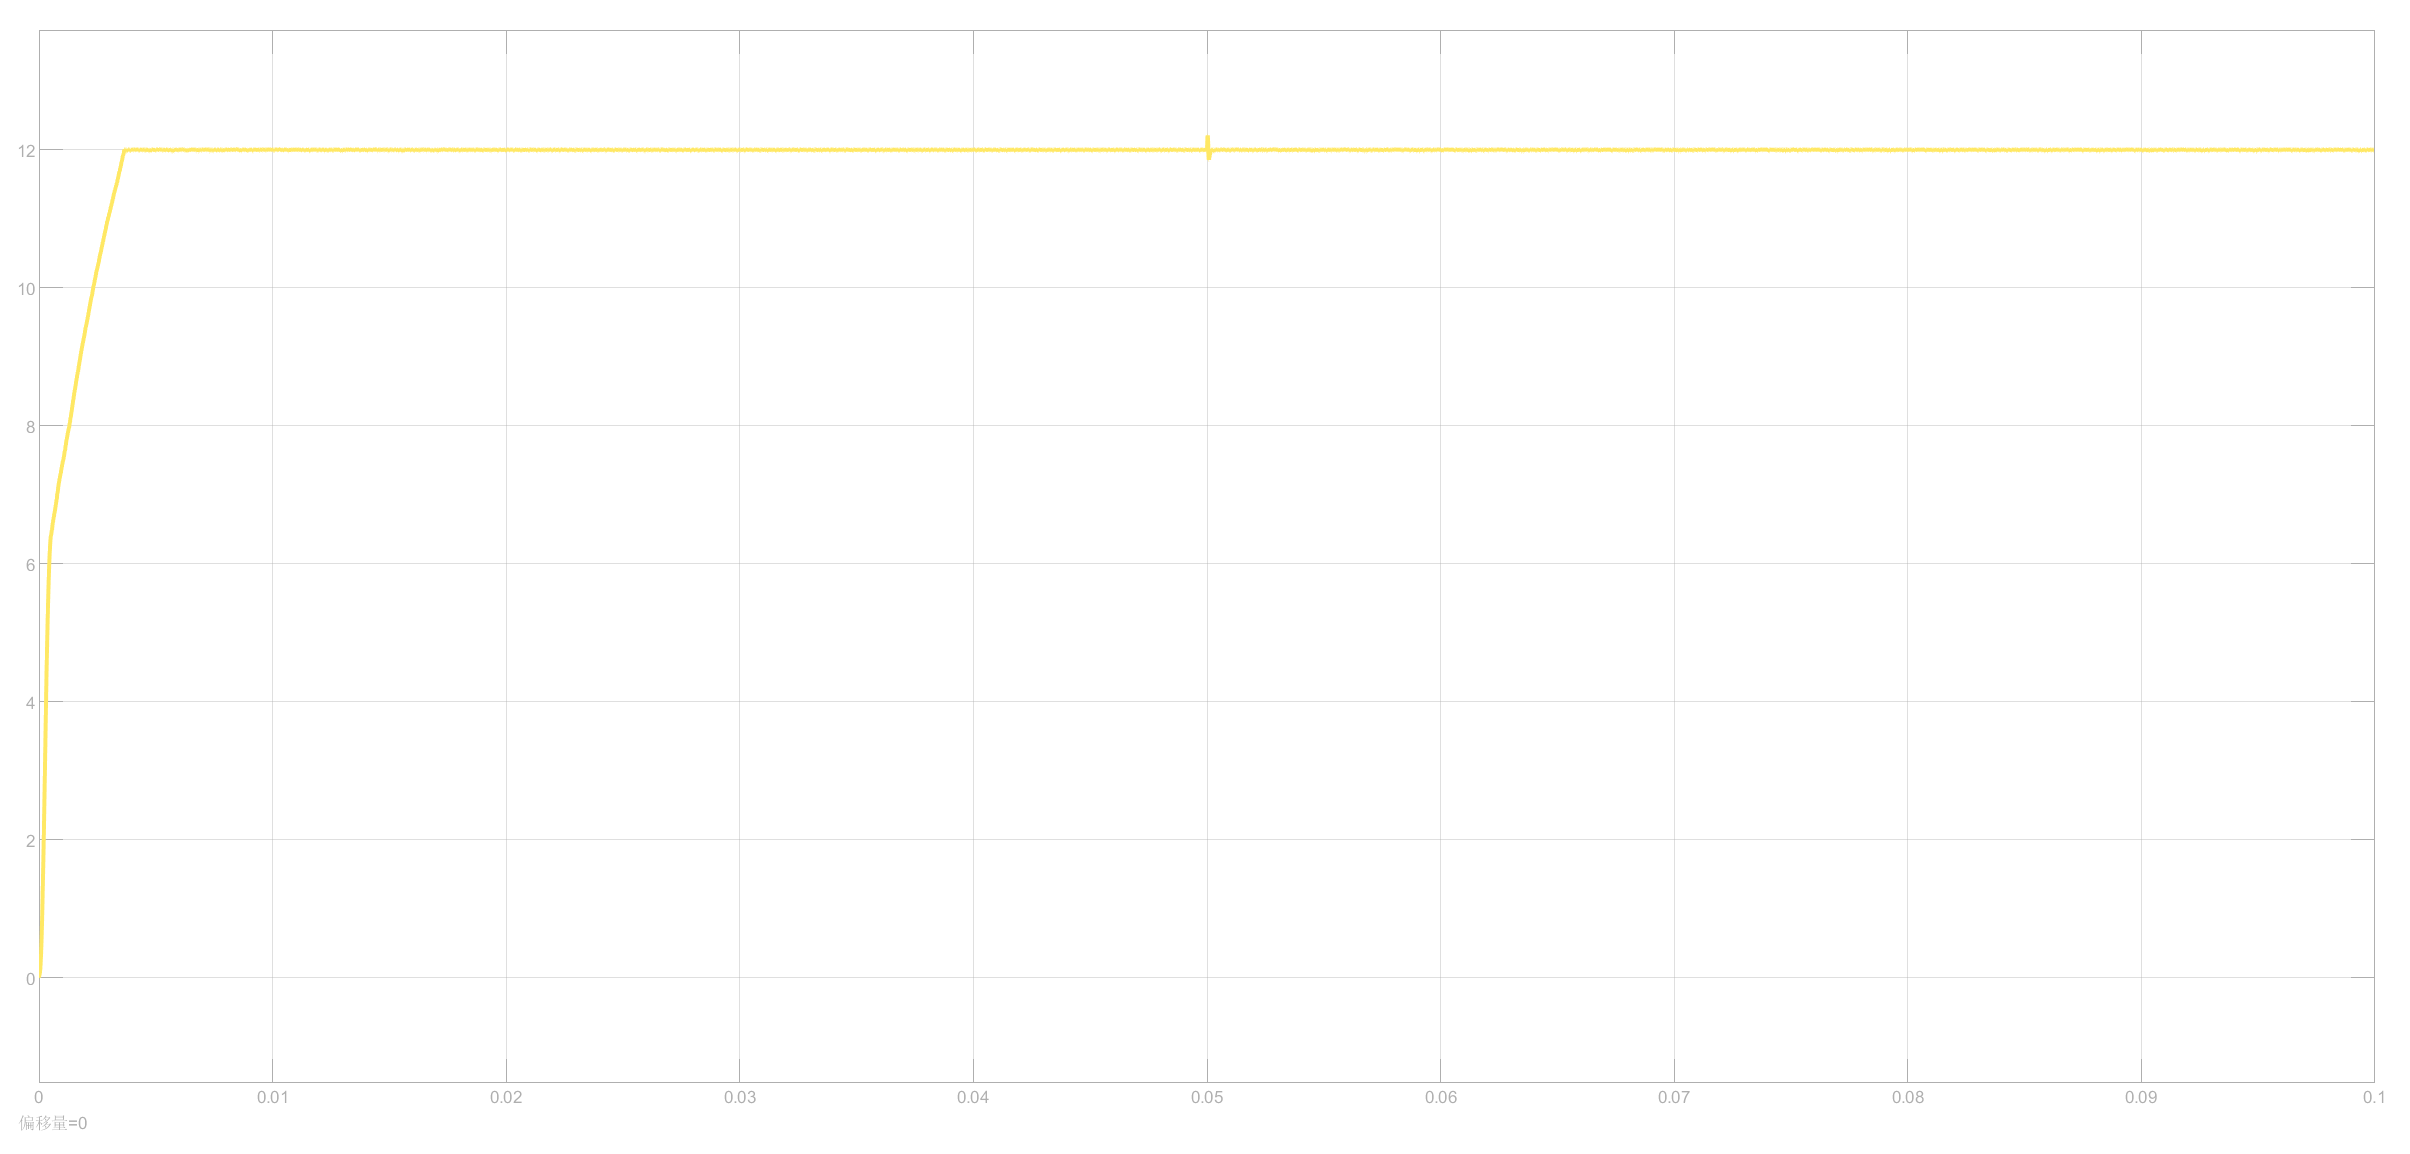
\includegraphics[width=0.8\textwidth]{image9.eps}
\caption{输入电压为52V，加入切载时，系统仿真结果}
\end{figure}

由信号统计可知，在$t=0.05s$处施加$10\%-100\%$的切载过程，输出电压超调量为$0.21V$，切载引起的电压跌落到$11.85V$,小于设计要求的$5\% \times 12V=0.6V$。

\textcircled{3}当输入电压为32V时

在稳态负载下仿真波形如下：
\newpage
\begin{figure}[htbp]
\centering  
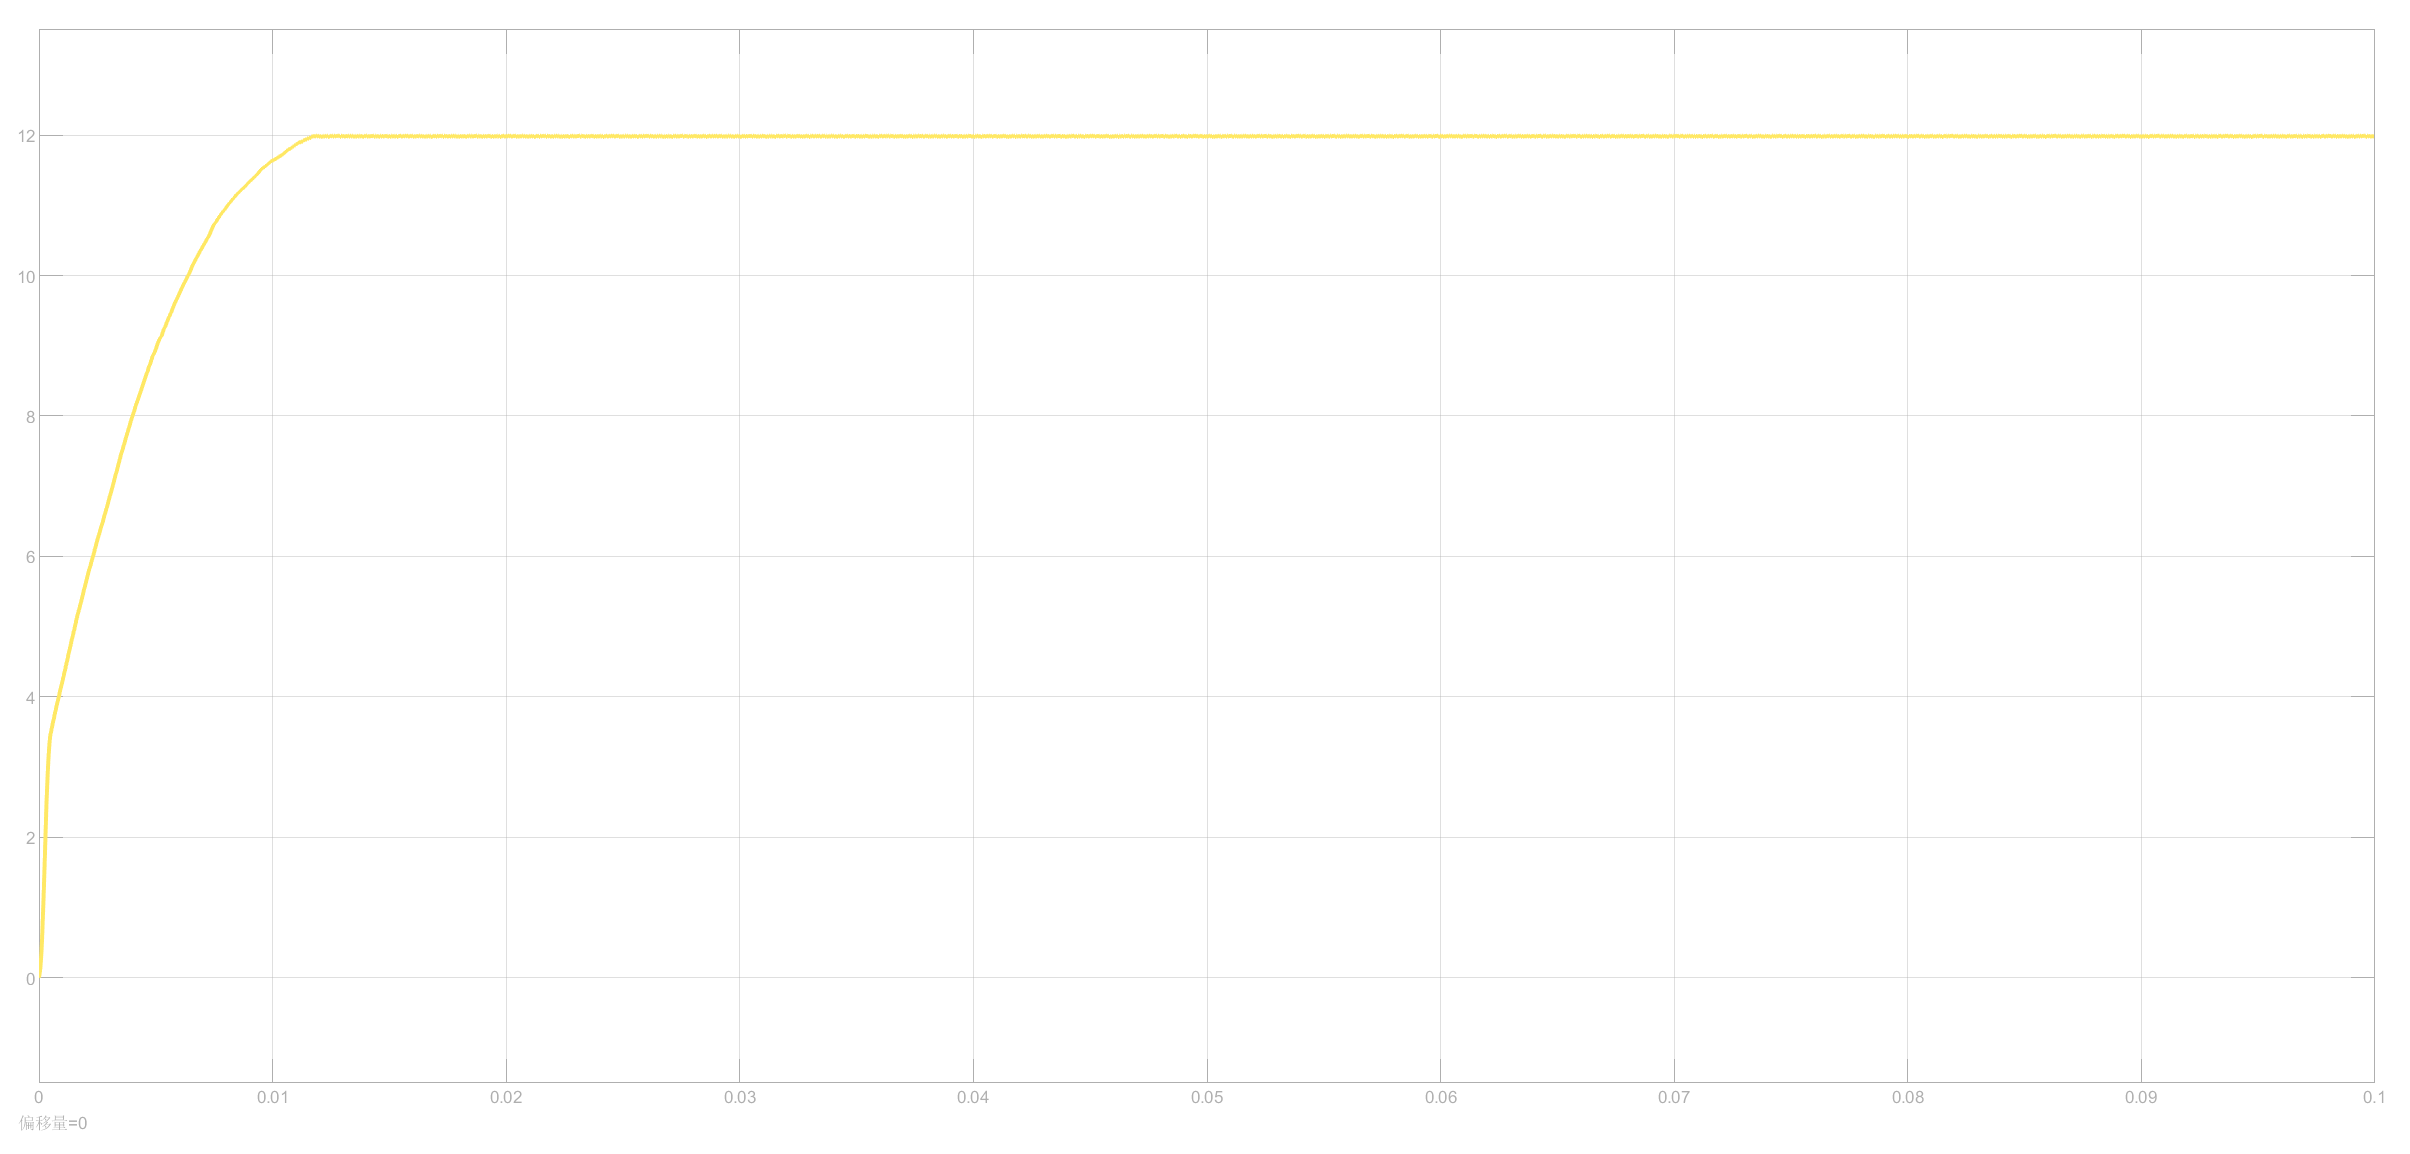
\includegraphics[width=0.8\textwidth]{image10.eps}
\caption{输入电压为32V，未加切载时，系统仿真结果}
\end{figure}

单独观察电压纹波：
\begin{figure}[h]
\centering  
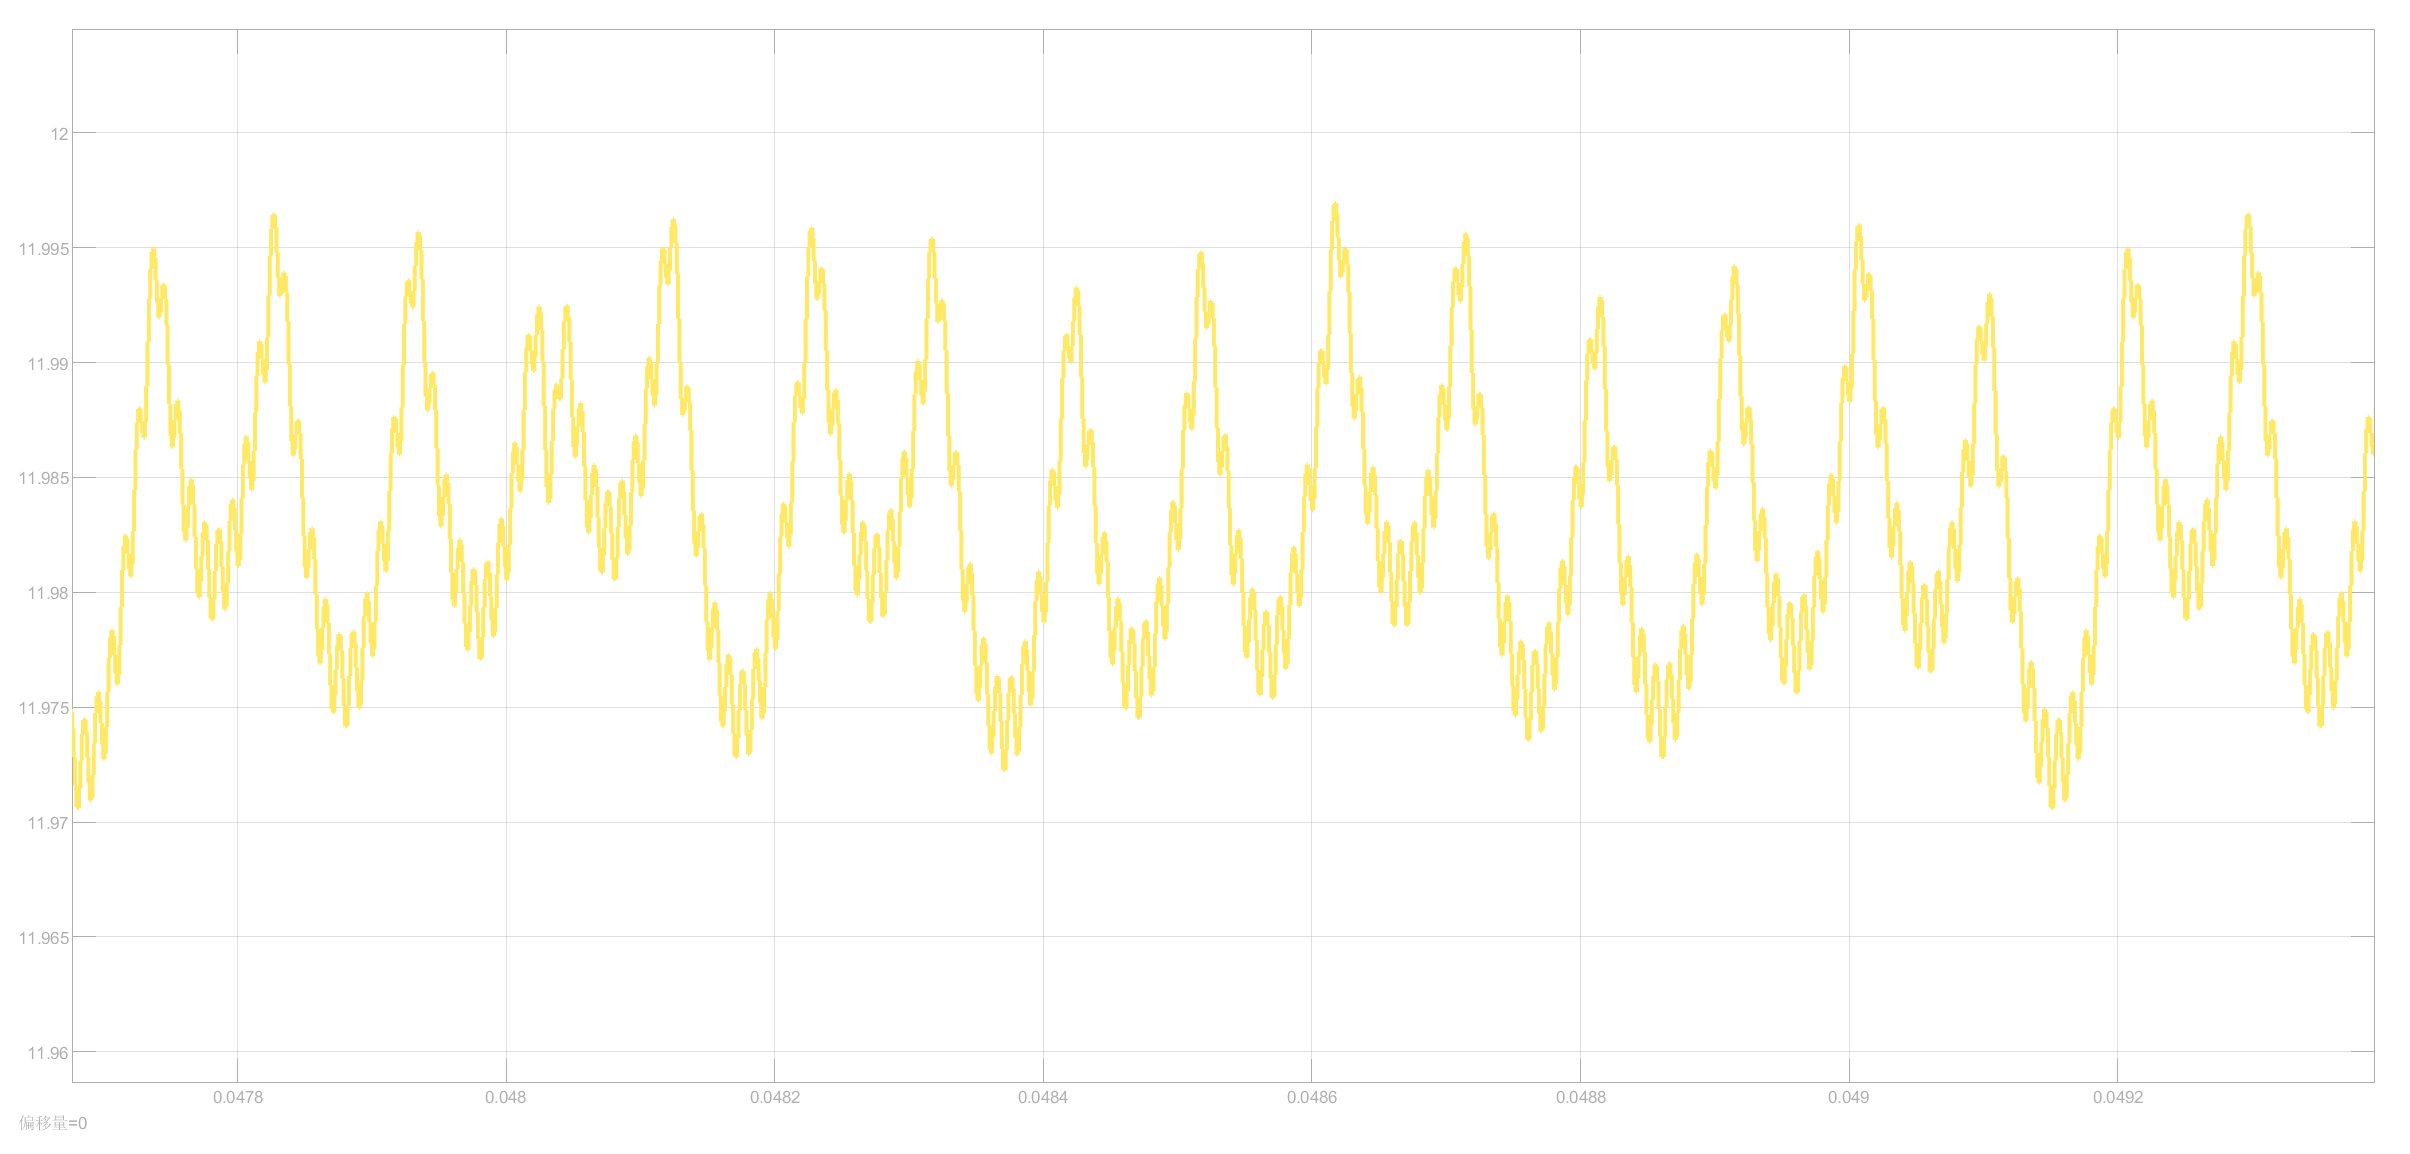
\includegraphics[width=0.8\textwidth]{image11.eps}
\caption{输出电压的纹波}
\end{figure}
\newpage
由信号统计可知，输出电压纹波为$26.34mV$，双电平测量振幅为$7.376mV$。

加入切载时，系统仿真结果如下：
\begin{figure}[htbp]
\centering  
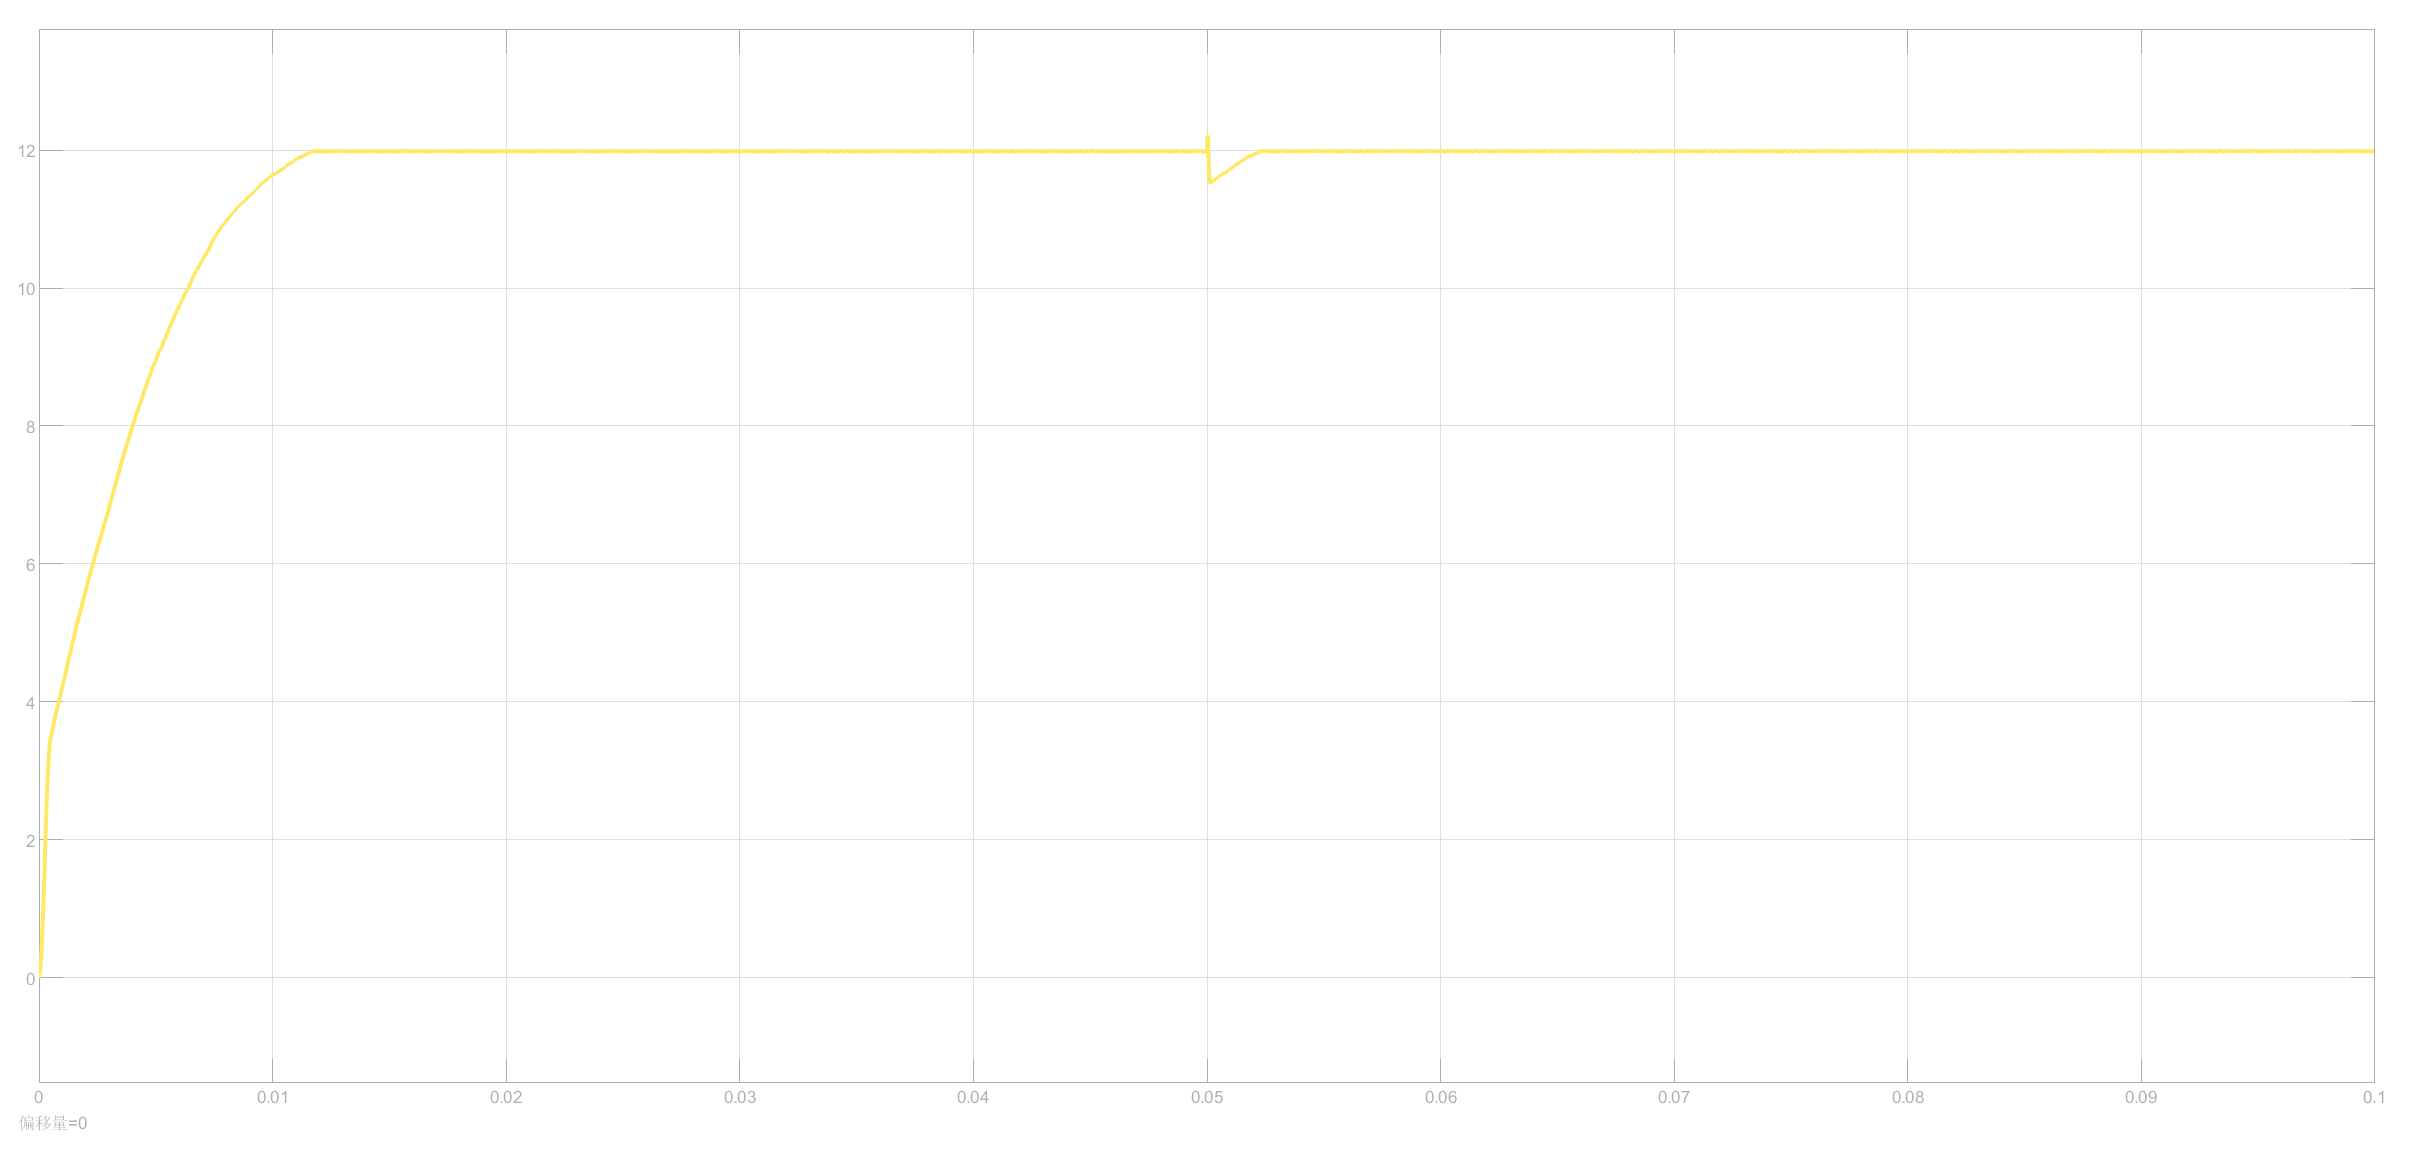
\includegraphics[width=0.8\textwidth]{image12.eps}
\caption{输入电压为32V，加入切载时，系统仿真结果}
\end{figure}

由信号统计可知，在$t=0.05s$处施加$10\%-100\%$的切载过程，输出电压超调量为$0.21V$，切载引起的电压跌落到$11.52V$,小于设计要求的$5\% \times 12V=0.6V$。

由输出波形可知，在不同的输入电压下，模糊控制器能够较好地控制 Buck 电路的输出电压，满足负载调整率$< 1\%$的设计要求。

\section{ Buck 电路的 PID 设计与仿真}
\subsection{设计框图}
\begin{figure}[htbp]
\centering
\includegraphics[width=0.8\textwidth]{0.png}
\caption{Buck 电路的 PID 控制器设计框图}
\end{figure}
其中:
\begin{itemize}
\item $G_c(s)$：补偿器的传递函数；
\item $G_m(s)$：PWM 的传递函数；
\item $G_{vd} (s)$：Buck 主电路由 IGBT 的输入到输出的传递函数；
\item $H(s)$：电压采样反馈回路的传递函数；
\item $G_{vs} (s)$：Buck 主电路由输入 Vin 到输出 Vo 的传递函数；
\item $Z_o$：负载阻抗；
\item $V_{ref}$：给定电压值；
\end{itemize}
\subsection{设计过程}
\textcircled{1}$H(s)$的确定

反馈回路的传递函数为
\begin{equation*}
    H(s)=1
\end{equation*}

\textcircled{2}$G_m(s)$的确定

在MATLAB仿真中，产生 PWM 信号的三角波幅值取为$1V$，开关频率取为$100kHz$，
则系统开关角频率为$\omega_{s}=6.28 \times 10^5rad/s$。
PWM 的传递函数为
\begin{equation*}
    G_m(s)=\frac{1}{V_m}=1
\end{equation*}

\textcircled{3}$G_{vd}(s)$的确定  

由 Buck 电路的小信号模型知 Buck 主电路由 IGBT 的输入到输出的传递函数为：
\begin{equation*}
G_{vd}(s) = \frac{Vin}{1 + s\frac{L}{Z0} + LCs^2}
\end{equation*}

为了适应输入电压的变化，取输入电压 $Vin = 42V$，$Z0 = 6 \Omega$ 代入数据得：
\begin{equation*}
G_{vd}(s) = \frac{42}{1.551 \times 10^{-8} s² + 5.5 \times 10^{-5} s + 1}
\end{equation*}

未加校正装置时的开环传递函数为
\begin{equation*}
G_0(s) = G_m(s)G_{vd}(s)H(s) = \frac{42}{1.551 \times 10^{-8} s² + 5.5 \times 10^{-5} s + 1}
\end{equation*}

未校正系统的谐振极点为$\omega_p = 8030.7 rad/s$，阻尼比为$\zeta = 0.2208$，品质因数为$Q = 2.265$。
阻尼后（受阻尼）谐振角频率（复极点的虚部）为
\begin{equation*}
\omega_r = \omega_p \sqrt{1 - 2\zeta^2} = 7836 rad/s
\end{equation*}
对应频率$f_r=\frac{\omega_r}{2\pi} = 1247.6 Hz$。
\newpage
作出未校正系统的 Bode 图如下所示：
\begin{figure}[htbp]
\centering
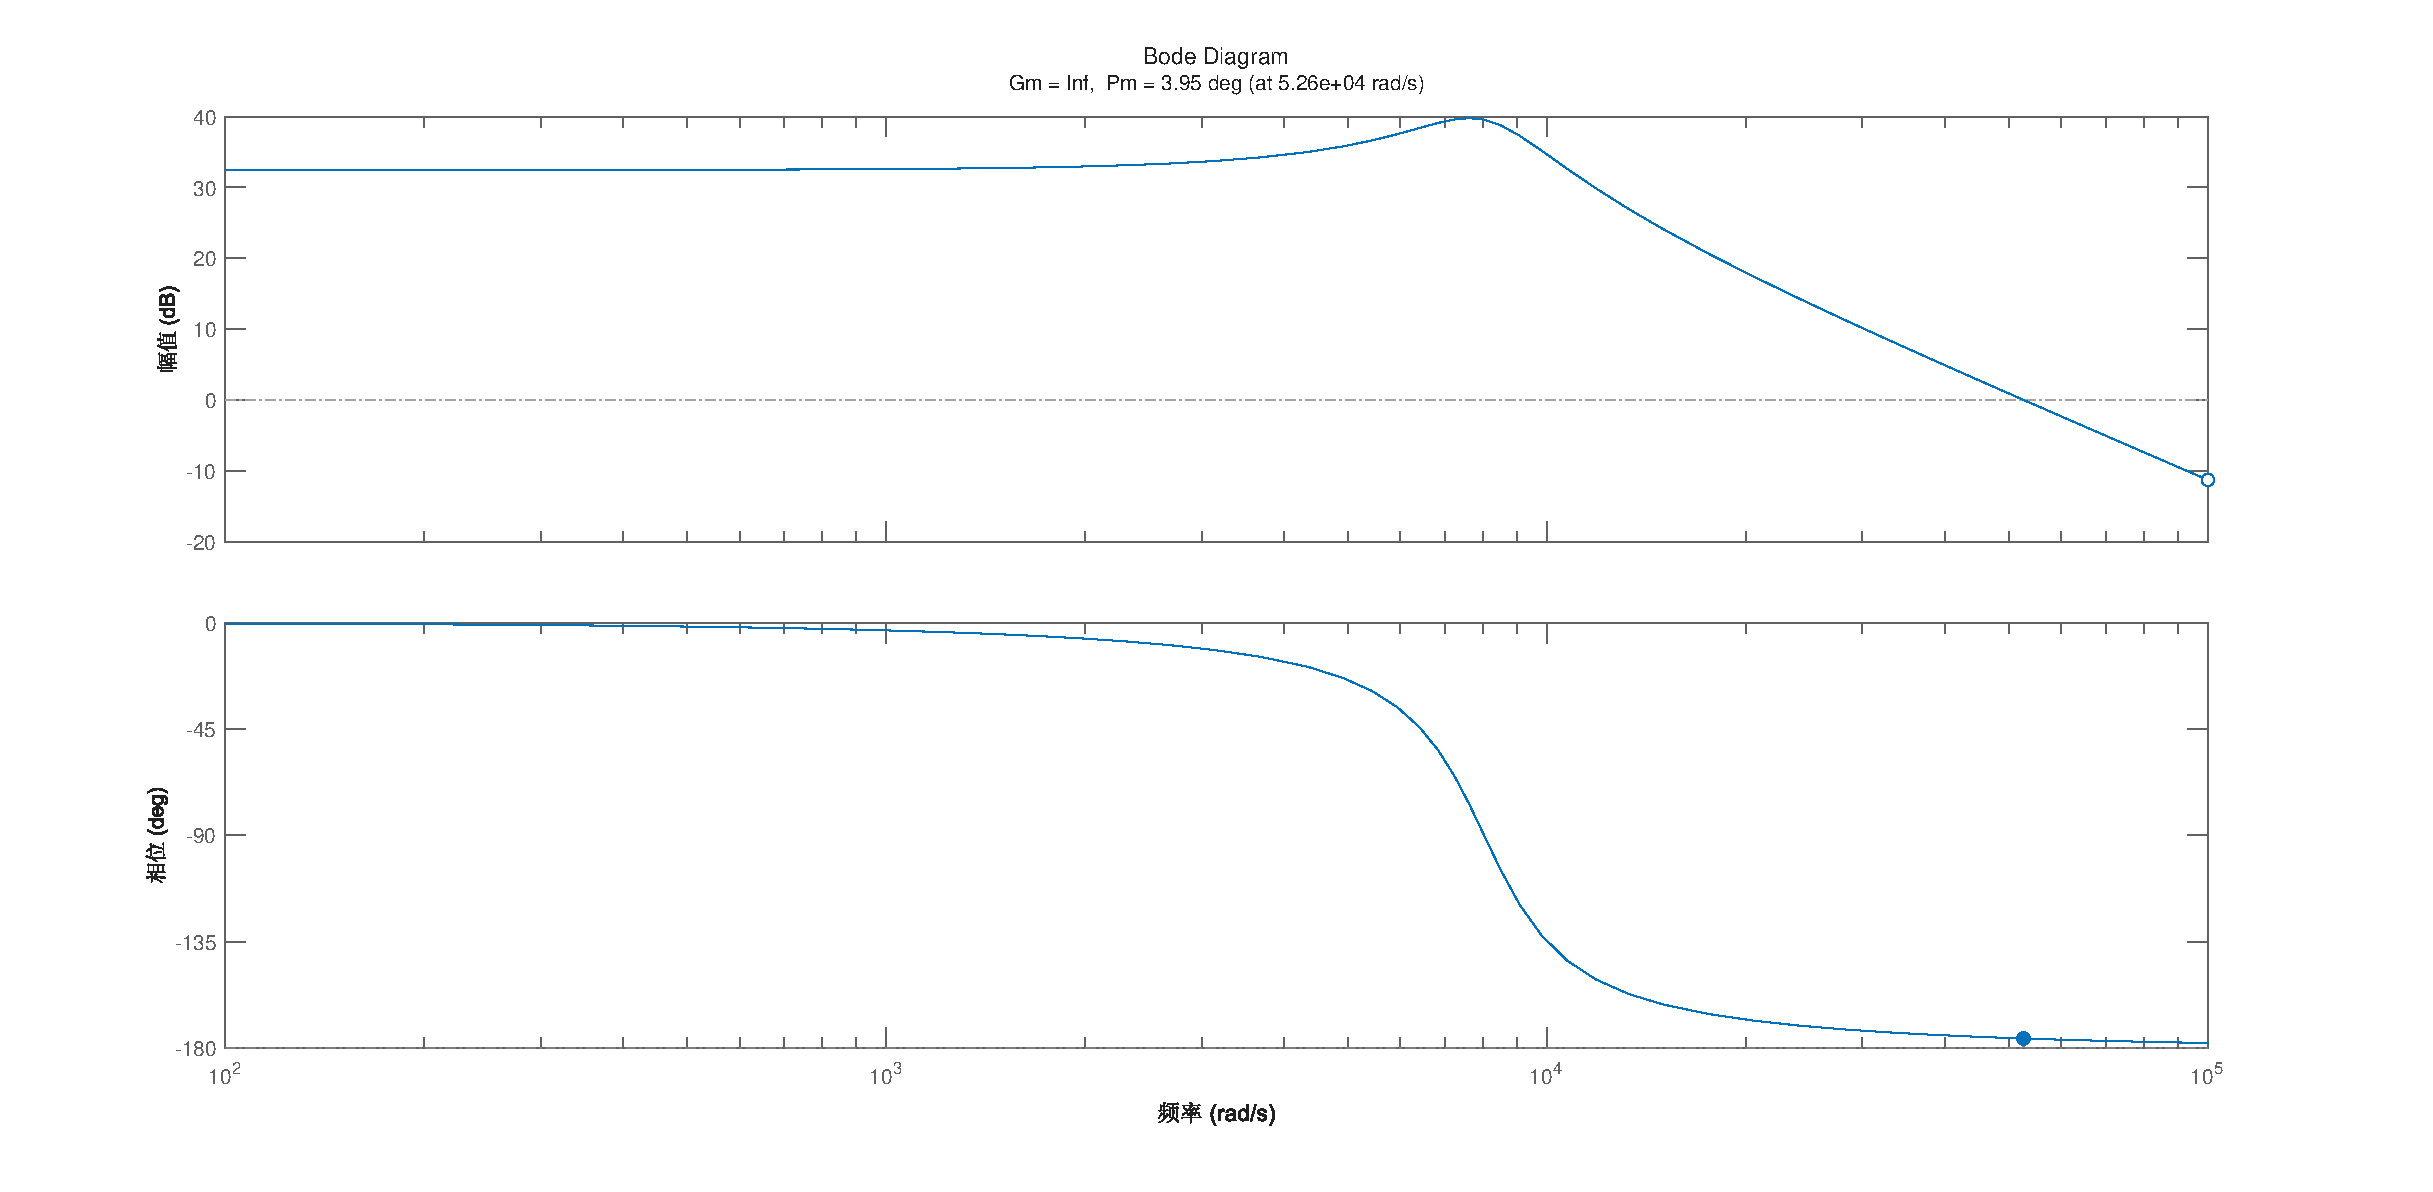
\includegraphics[width=0.8\textwidth]{bode1.eps}
\caption{未校正系统的 Bode 图}
\end{figure}

由bode图知系统的增益裕度 GM 为无穷大，相角裕度 PM 为$3.95$度，截止频率$\omega_0$为$5.26 \times 10^{4}rad/s$。
增益裕度过小，但是相角裕度偏小，开环系统存在振荡环节，电源和负载的扰动容易使系统不稳定。

\textcircled{4}闭环补偿器$G_c(s)$的设计

理想开环传递函数的频幅特性：

1、低频段：它主要影响系统的稳态性能。
对于开关调节系统，理想的低频特性是直流增益无限大，以$ - 20dB/dec $的斜率下降。
符合理想条件时，系统的稳态误差等于零。

2、中频段：中频段大致是指幅频特性以$ - 20dB/dec $斜率下降并穿越$ 0dB $线的频段。
中频段的宽度与系统的动态稳定性密切相关。
越宽则相位裕量越大，穿越频率越大，系统的响应速度越快但超调量越大。
对于开关调节系统，过高的穿越频率可能导致高频开关频率及其谐波和寄生振荡引起的高频分量得不到有效地抑制，系统仍然不能稳定工作。

3、高频段：高频段距穿越频率一般较远，反映了系统对高频干扰信号的抑制能力。
高频段幅频特性衰减越快，系统的抗干扰能力越强，对于开关调节系统，理想高频特性应以$ - 40dB/dec $的斜率下降。

下面给出设置零极点的规则:

\textcircled{1}在原点处设置一个极点，使系统变成一阶系统，用来提升低频增益，降低稳态误差，即
\[ \omega_{p0} = 0 \]

\textcircled{2}在谐振极点频率的\(\tfrac{1}{2}\)处设置两个零点，用于提升系统bode图在中频段的斜率，使系统在中频段以理想的$-20dB/dec$的斜率通过坐标轴，同时会使系统的截止频率增加，由bode图可以看到当截止频率增加时，系统的幅值裕度增大，由系统时域与频域的联系知，系统的截止频率增加时会使系统的调节时间减小，使系统的动态响应提高，系统幅值裕度增大时会使系统的系统超调量减小。即
\[ \omega_{z1} = 3.918 \times 10^3\mathrm{rad/s}, \quad \omega_{z2} = 3.918 \times 10^3\mathrm{rad/s} \]

\textcircled{3}为了使系统高频噪声尽快衰减，在开关频率的\(\tfrac{1}{2}\)处设置一个极点，用于衰减系统的高频噪声，提高系统的抗干扰能力。即
\[ \omega_{p1} = 3.14 \times 10^5\mathrm{rad/s} \]

\textcircled{4}校正后系统的截止频率一般为系统开关频率的\(\tfrac{1}{10}-\tfrac{1}{5}\)，在这里取系统开关频率的$1/10$，即校正后系统的截止频率为：
\[ \omega_{c1} = 6.28 \times 10^4\mathrm{rad/s} \]

综合\textcircled{1}\textcircled{2}\textcircled{3}\textcircled{4}得闭环补偿器的传递函数\(G_c(s)\)为：
\[ G_c(s) = K \frac{(2.5523 \times 10^{-4}s + 1)(2.5523 \times 10^{-4}s + 1)}{s(3.184 \times 10^{-6}s + 1)} \]

其中\( K \)为开环增益。由系统的幅值条件可知：
\[
\left| G_0(\omega_{c1}) G_c(\omega_{c1}) \right| = 1
\]
解得\( K = 356.51 \)，则闭环补偿器的传递函数为：
\[ G_c(s) = 356.51 \times \frac{(2.5523 \times 10^{-4}s + 1)(2.5523 \times 10^{-4}s + 1)}{s(3.184 \times 10^{-6}s + 1)} \]

以下是MATLAB代码：
\begin{lstlisting}[language=Matlab,frame=single]
% ---------- 参数与传函定义 ----------
s = tf('s');

% Plant G0(s)
G0 = 42 / (1.551e-8*s^2 + 5.5e-5*s + 1);

% Compensator (without k)
a = 2.5523e-4;
b = 3.184e-6;
C0 = (1 + a*s)^2 / ( s*(1 + b*s) );

% 目标交叉频率
fc = 10e3; wc = 2*pi*fc;

% 计算k：使 |k * G0(jwc) * C0(jwc)| = 1
G0jw = freqresp(G0, wc);
C0jw = freqresp(C0, wc);
k = 1 / ( abs(G0jw) * abs(C0jw) );
fprintf('Computed k = %.6f\n', k);

% 最终补偿器
C = k * C0;

% 显示传递函数
disp('Compensator C(s):'); C

% 画Bode并标注Margin
figure;
margin(G0); hold on;
margin(C*G0);
grid on;
title('Plant (blue) and Compensated Open-loop (orange)');
legend('Plant','Compensated Open-loop');

% 计算并显示相位裕度
[GM,PM,Wgm,Wpm] = margin(C*G0);
fprintf('Phase margin = %.2f deg at f = %.2f Hz\n', PM, Wpm/(2*pi));
fprintf('Gain margin (dB) = %.2f at W = %.2f rad/s\n', 20*log10(GM), Wgm);
\end{lstlisting}

作出校正后系统的 Bode 图如下所示：
\begin{figure}[htbp]
\centering
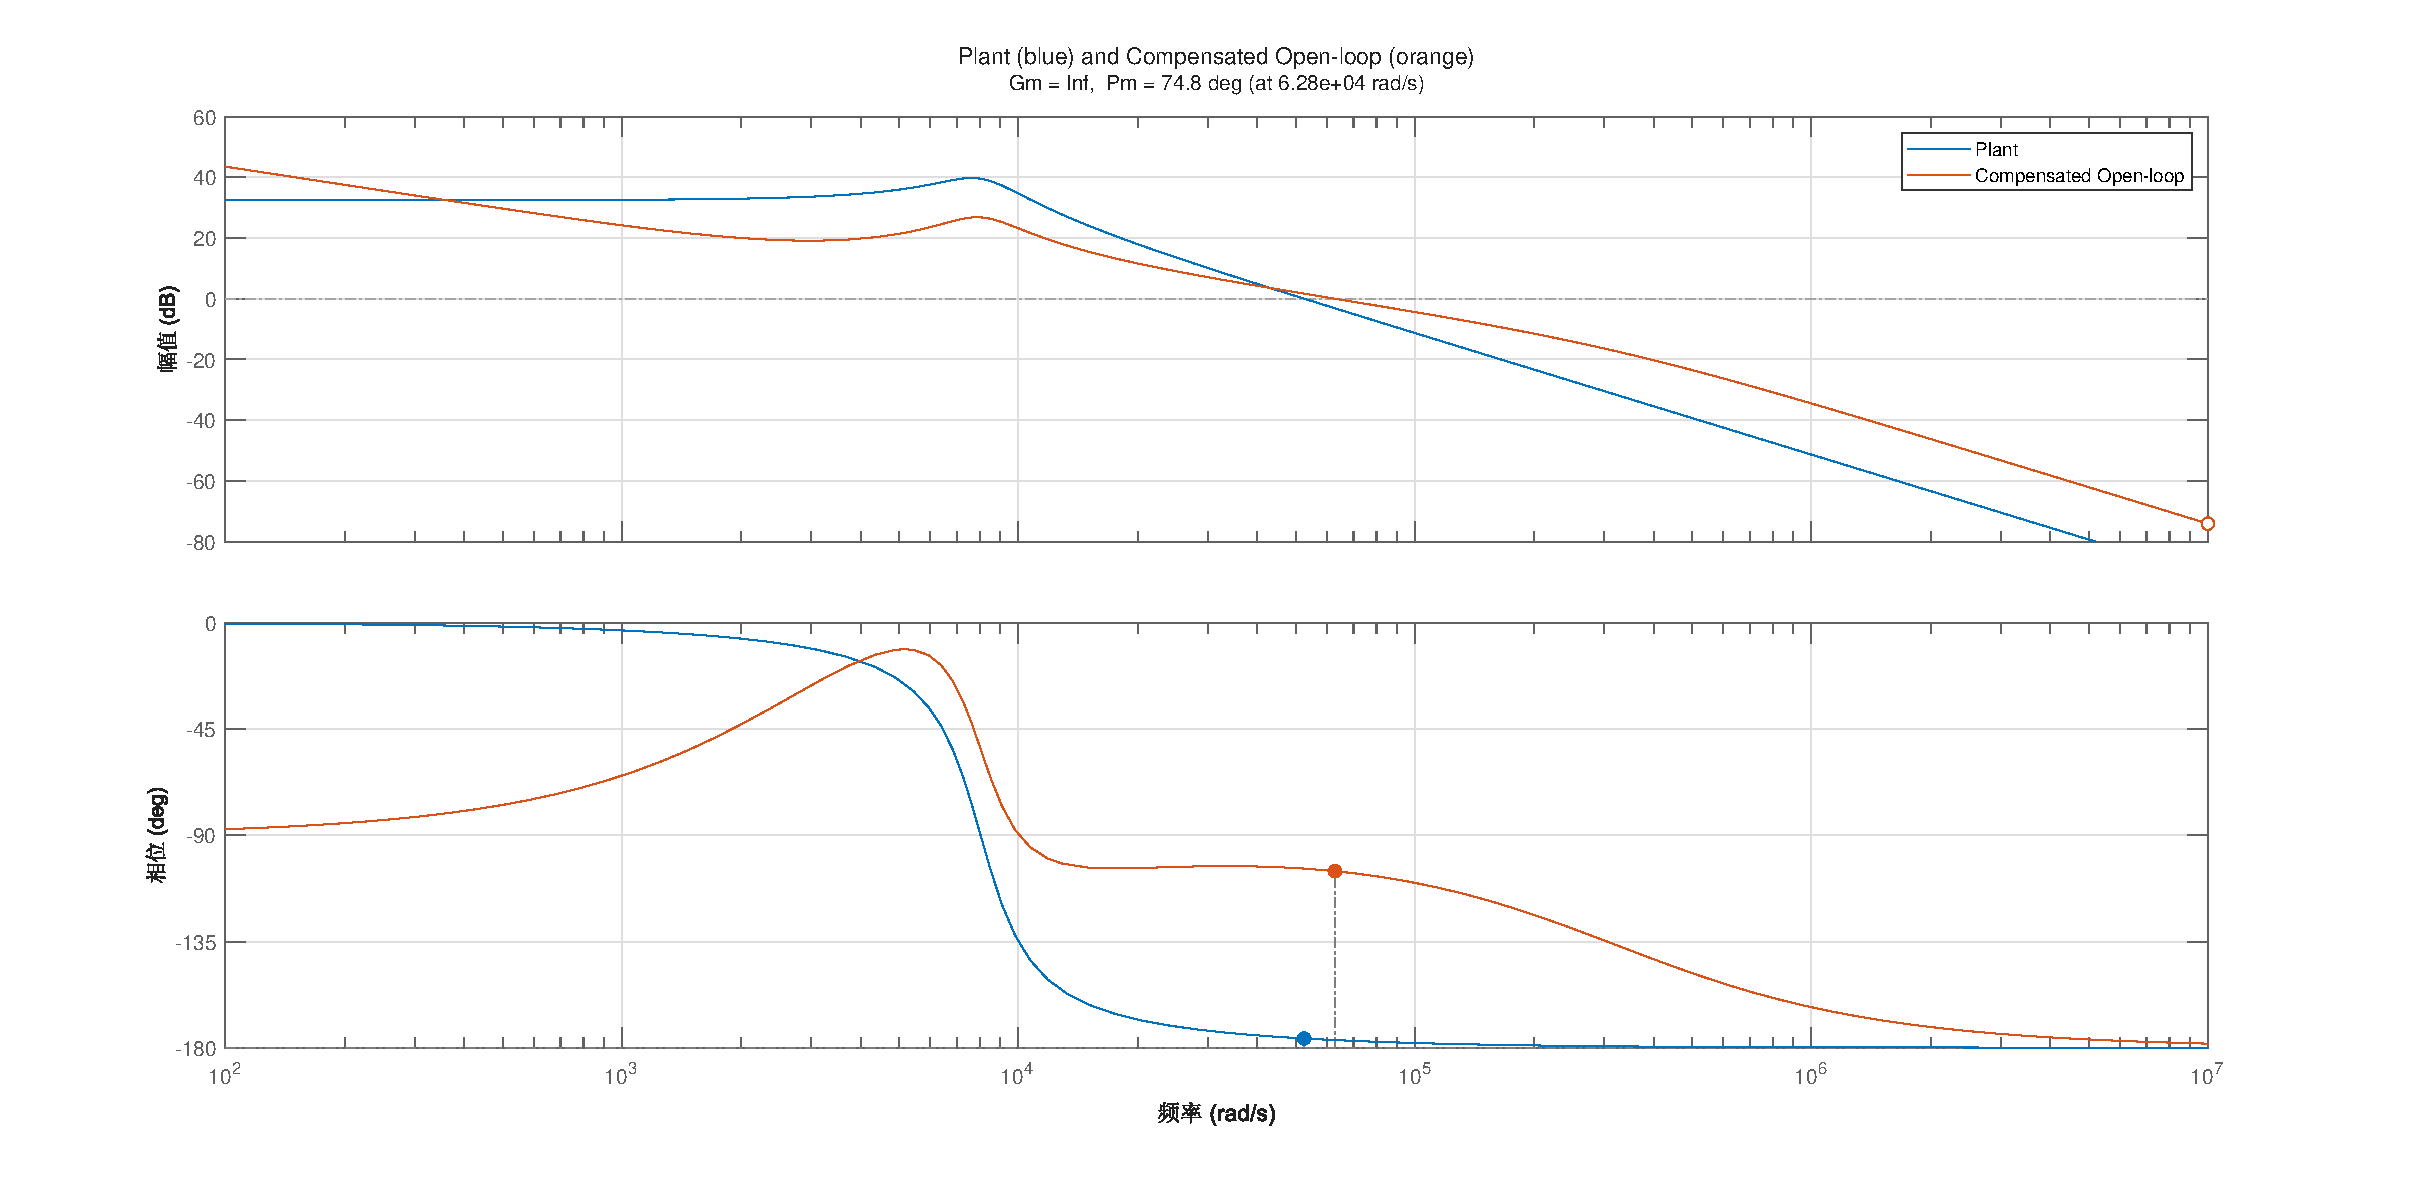
\includegraphics[width=0.8\textwidth]{image13.eps}
\caption{校正后系统的 Bode 图}
\end{figure}

由bode图知系统的增益裕度 GM 为无穷大，相角裕度 PM 为$74.8$度，截止频率$\omega_0$为$6.28 \times 10^{4}rad/s$。
因此我们需要微调补偿器的参数，使得系统的相角裕度 PM 接近$60$度。

根据上述步骤并循环求解，得到的推荐参数为：
\[
a = 7.807259\times10^{-5},\qquad b = 3.184\times10^{-6},
\]
并在 $f_c=12\ \mathrm{kHz}$ 时求得放大系数
\[
\,k \approx 4519.3\,
\]
因此最终补偿器为
\begin{equation*}
  C(s) \approx 4519.3 \times \frac{\bigl(1 + 7.807259\times10^{-5}\,s\bigr)^2}{s\bigl(1 + 3.184\times10^{-6}\,s\bigr)}.
\end{equation*}

用该补偿器与被控对象构成的开环，在 $f_c=12\ \mathrm{kHz}$ 处计算得到的相角裕度约为
\[
\mathrm{PM} \approx 59.9^\circ,
\]
满足所希望的 $45^\circ\sim60^\circ$ 要求。

用于验证的 MATLAB 代码如下：
\begin{lstlisting}[language=Matlab,frame=single]
% Plant and compensator (verify fc = 12 kHz)
s = tf('s');
G0 = 42 / (1.551e-8*s^2 + 5.5e-5*s + 1);

% suggested compensator parameters
a = 7.807259e-5;
b = 3.184e-6;
C0p = (1 + a*s)^2 / ( s*(1 + b*s) );

% target fc
fc = 12e3; wc = 2*pi*fc;
% compute k so that |k*G0(jwc)*C0p(jwc)| = 1
G0jw = freqresp(G0, wc);
C0pjw = freqresp(C0p, wc);
k = 1 / ( abs(G0jw) * abs(C0pjw) );
fprintf('Computed k = %.4f\n', k);

C = k * C0p;
% show TF and margins
disp('Compensator C(s):'); C
figure; margin(G0); hold on; margin(C*G0); grid on;
title('Plant (blue) and Compensated Open-loop (orange)');
[GM,PM,Wgm,Wpm] = margin(C*G0);
fprintf('Phase margin = %.2f deg at f = %.2f Hz\n', PM, Wpm/(2*pi));
\end{lstlisting}

作出校正后系统的 Bode 图如下所示：
\begin{figure}[htbp]
\centering
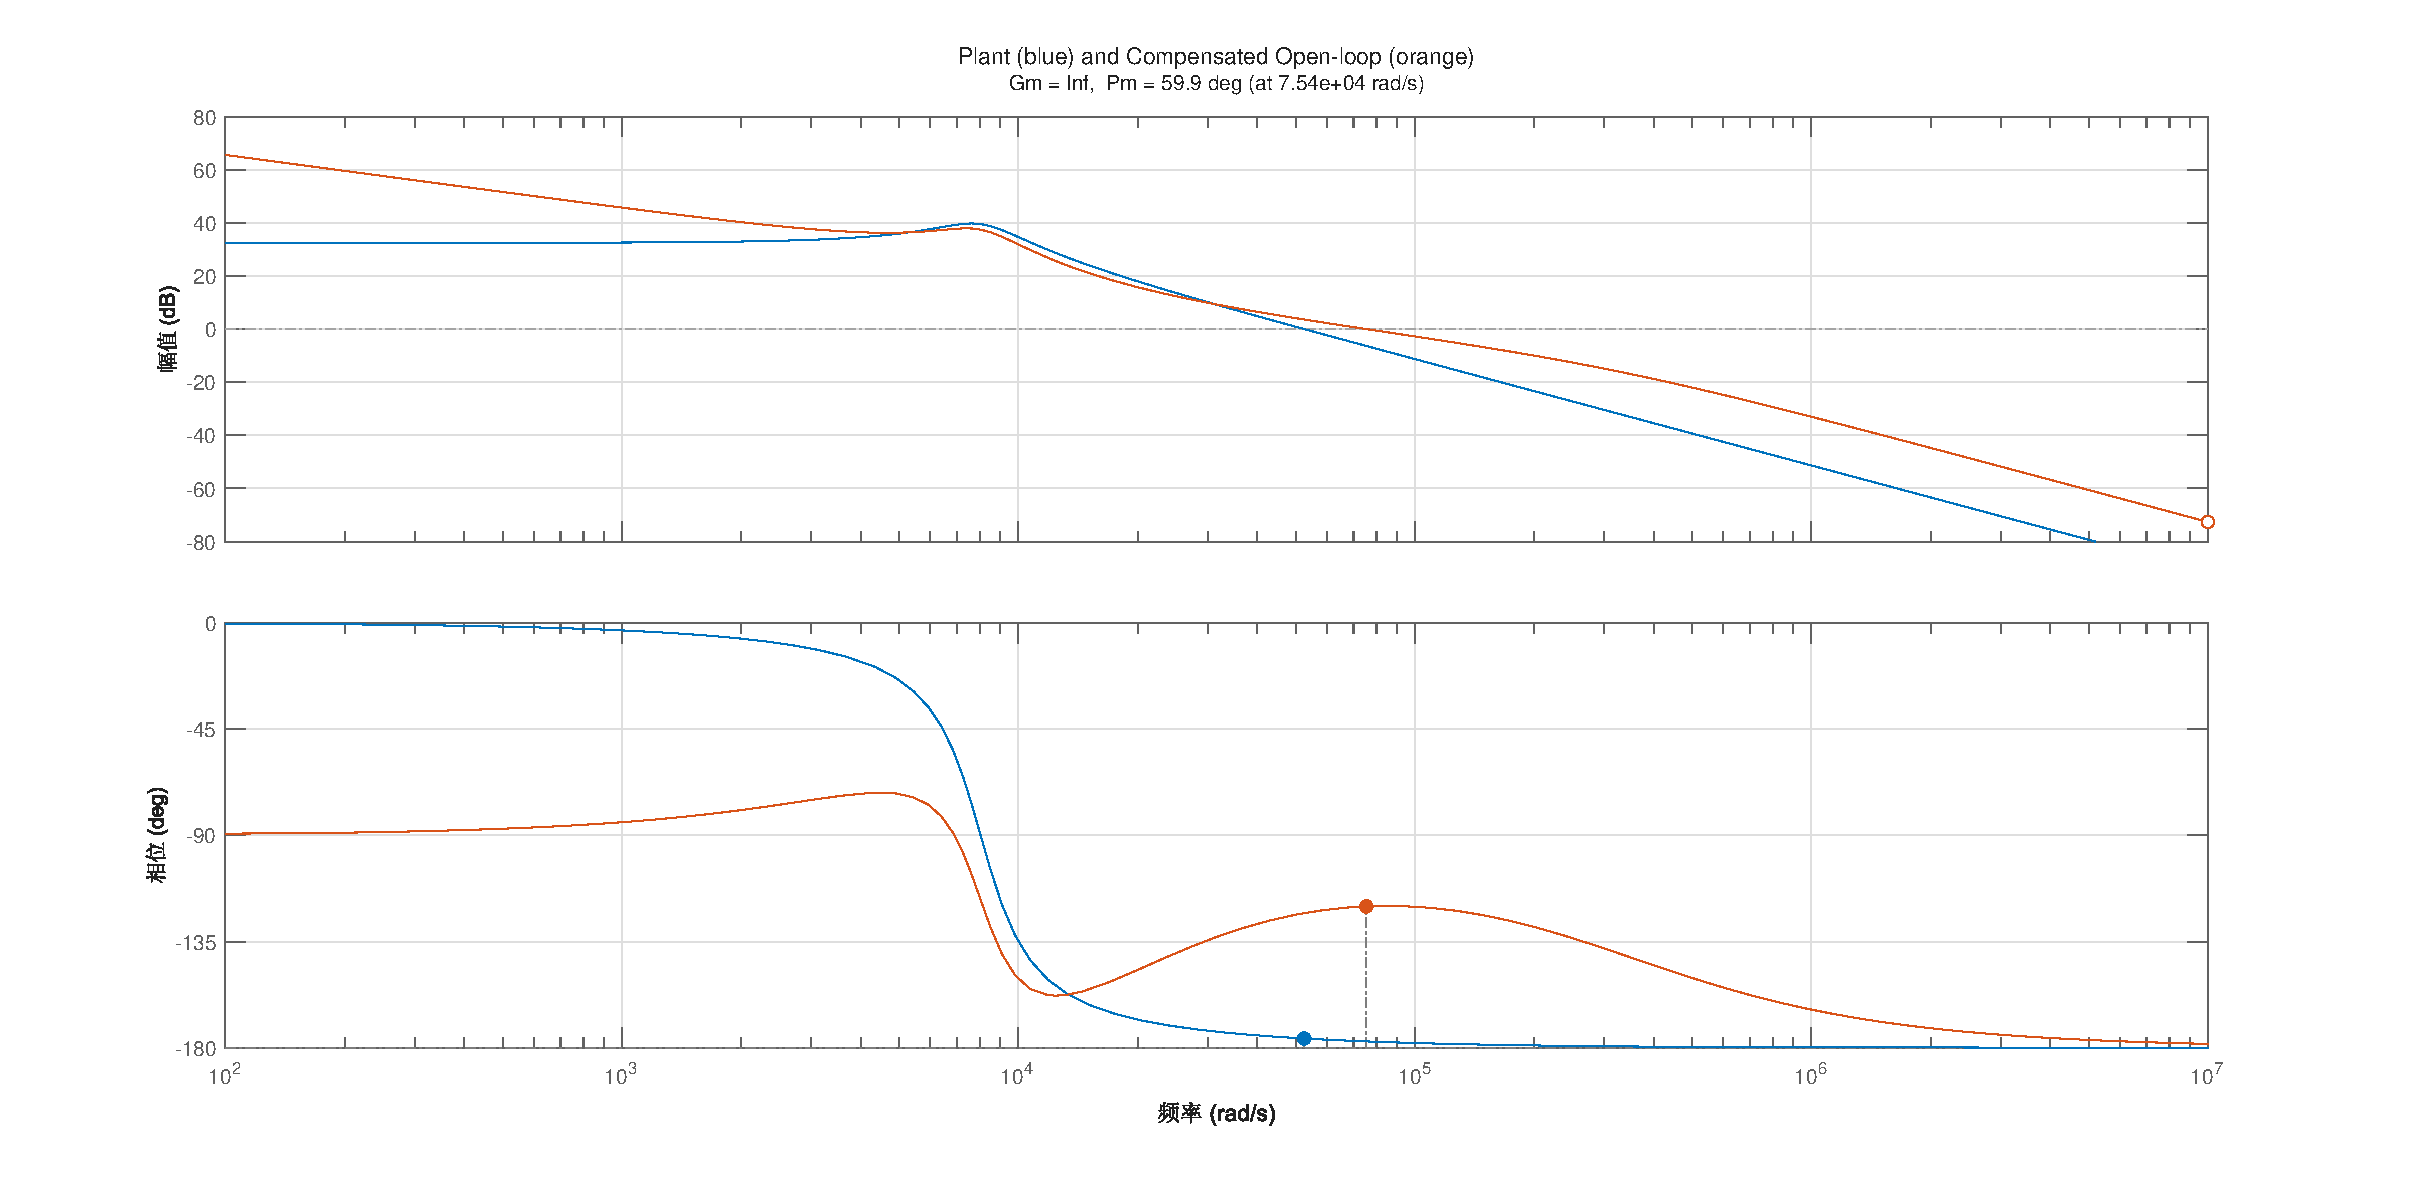
\includegraphics[width=0.8\textwidth]{image14.eps}
\caption{校正后系统的 Bode 图}
\end{figure}

下面是补偿器分解为并联 PID 的推导：

本设计中给定的补偿器形式为
\begin{equation*}
  C(s)=k\cdot\frac{(1+a s)^2}{s(1+b s)}.
\end{equation*}
我们希望将其写成并联的 PID 形式（含带滤波的微分支）：
\begin{equation*}
  C(s)=\frac{K_i}{s} + K_p + \frac{K_d\,s}{1+b s},
\end{equation*}
其中 \(K_i\) 为积分增益，\(K_p\) 为比例增益，\(K_d\) 为微分增益，且微分分支带与原式相同的滤波时间常数 \(b\)。

化简得到等价关系
\[
\frac{K_i(1+b s) + K_p s(1+b s) + K_d s^2}{s(1+b s)}
 \equiv \frac{k(1+2a s + a^2 s^2)}{s(1+b s)}.
\]
比较分子关于 \(s\) 各次幂的系数，得到代数方程组：
\begin{align*}
  s^0:\quad & K_i = k,\\
  s^1:\quad & K_i b + K_p = 2 k a,\\
  s^2:\quad & K_p b + K_d = k a^2.
\end{align*}
由此可解得显式解析式：
\begin{equation*}
  \,K_i = k,\qquad
        K_p = k(2a - b),\qquad
        K_d = k a^2 - K_p b \,
\end{equation*}
注意代入 \(K_p\) 后，上式可化为更简洁的形式
\[
K_d = k\bigl(a^2 - b(2a-b)\bigr) = k(a-b)^2.
\]


利用前面设计得到的参数
\[
a = 7.807259\times10^{-5},\qquad
b = 3.184\times10^{-6},\qquad
k \approx 4519.3,
\]
代入得：
\begin{align*}
  K_i &= k \approx 4519.3,\\[4pt]
  K_p &= k(2a-b) \approx 4519.3\cdot(2\cdot7.807259\times10^{-5}-3.184\times10^{-6})
      \approx 0.691,\\[4pt]
  K_d &= k(a-b)^2 \approx 4519.3\cdot(7.807259\times10^{-5}-3.184\times10^{-6})^2
      \approx 2.53\times10^{-5}.
\end{align*}
\newpage
Buck 电路的 PID 控制器Simulink仿真模型如下图所示：

\begin{figure}[htbp]
\centering  
\includegraphics[width=0.8\textwidth]{8.png}
\caption{Buck 电路的 PID 控制仿真模型}
\end{figure}

\textcircled{1}当输入电压为42V时

在稳态负载下仿真波形如下：
\begin{figure}[htbp]
\centering  
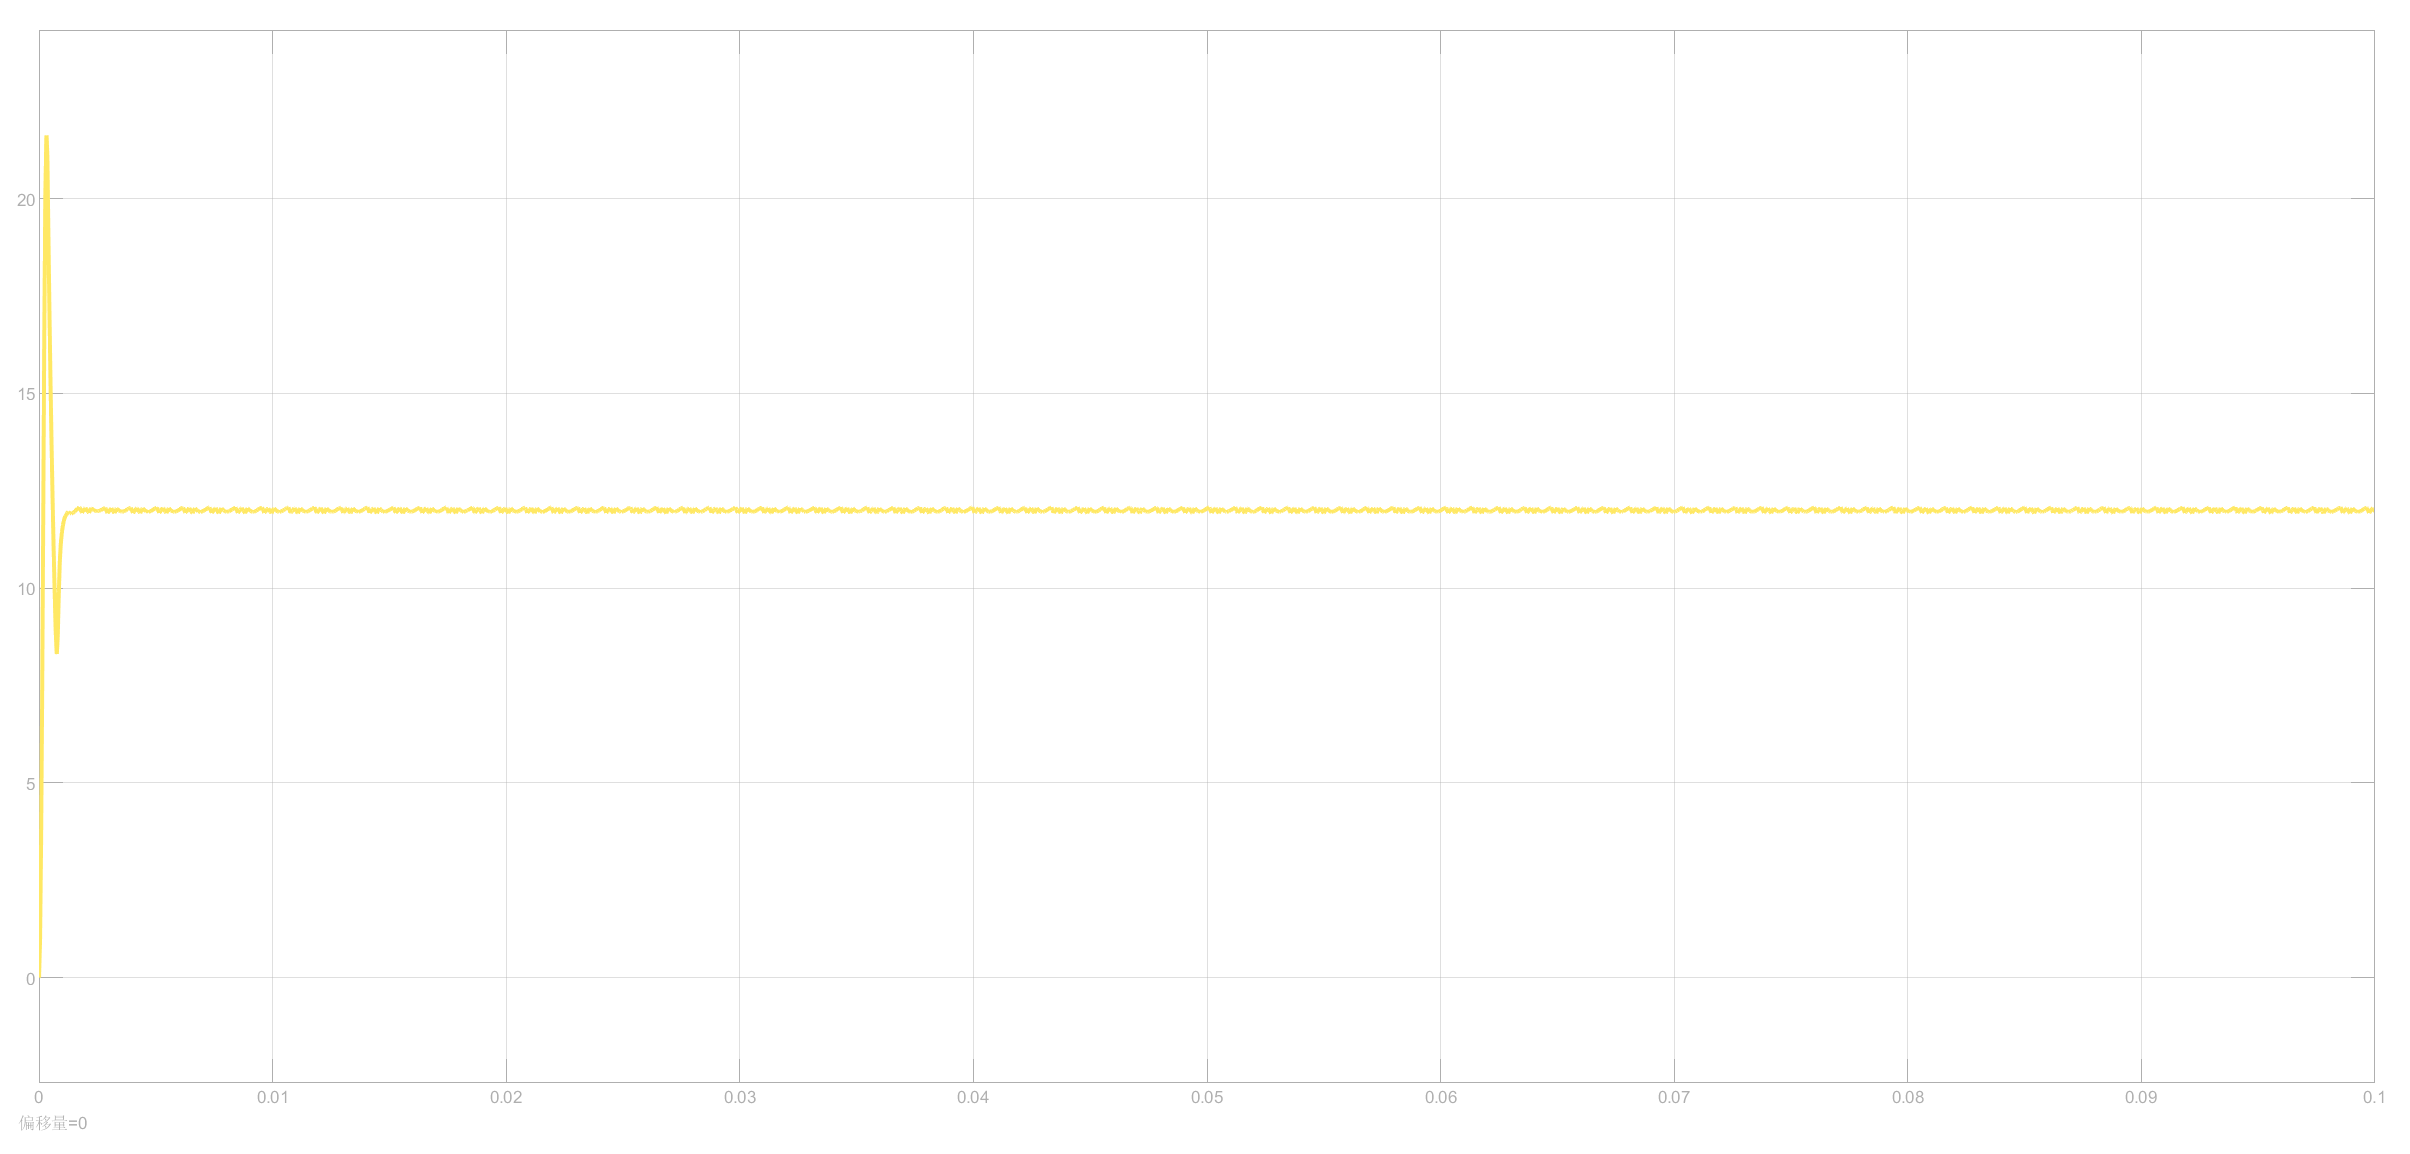
\includegraphics[width=0.8\textwidth]{image15.eps}
\caption{输入电压为42V，未加切载时，系统仿真结果}
\end{figure}
\newpage
单独观察电压纹波：
\begin{figure}[h]
\centering  
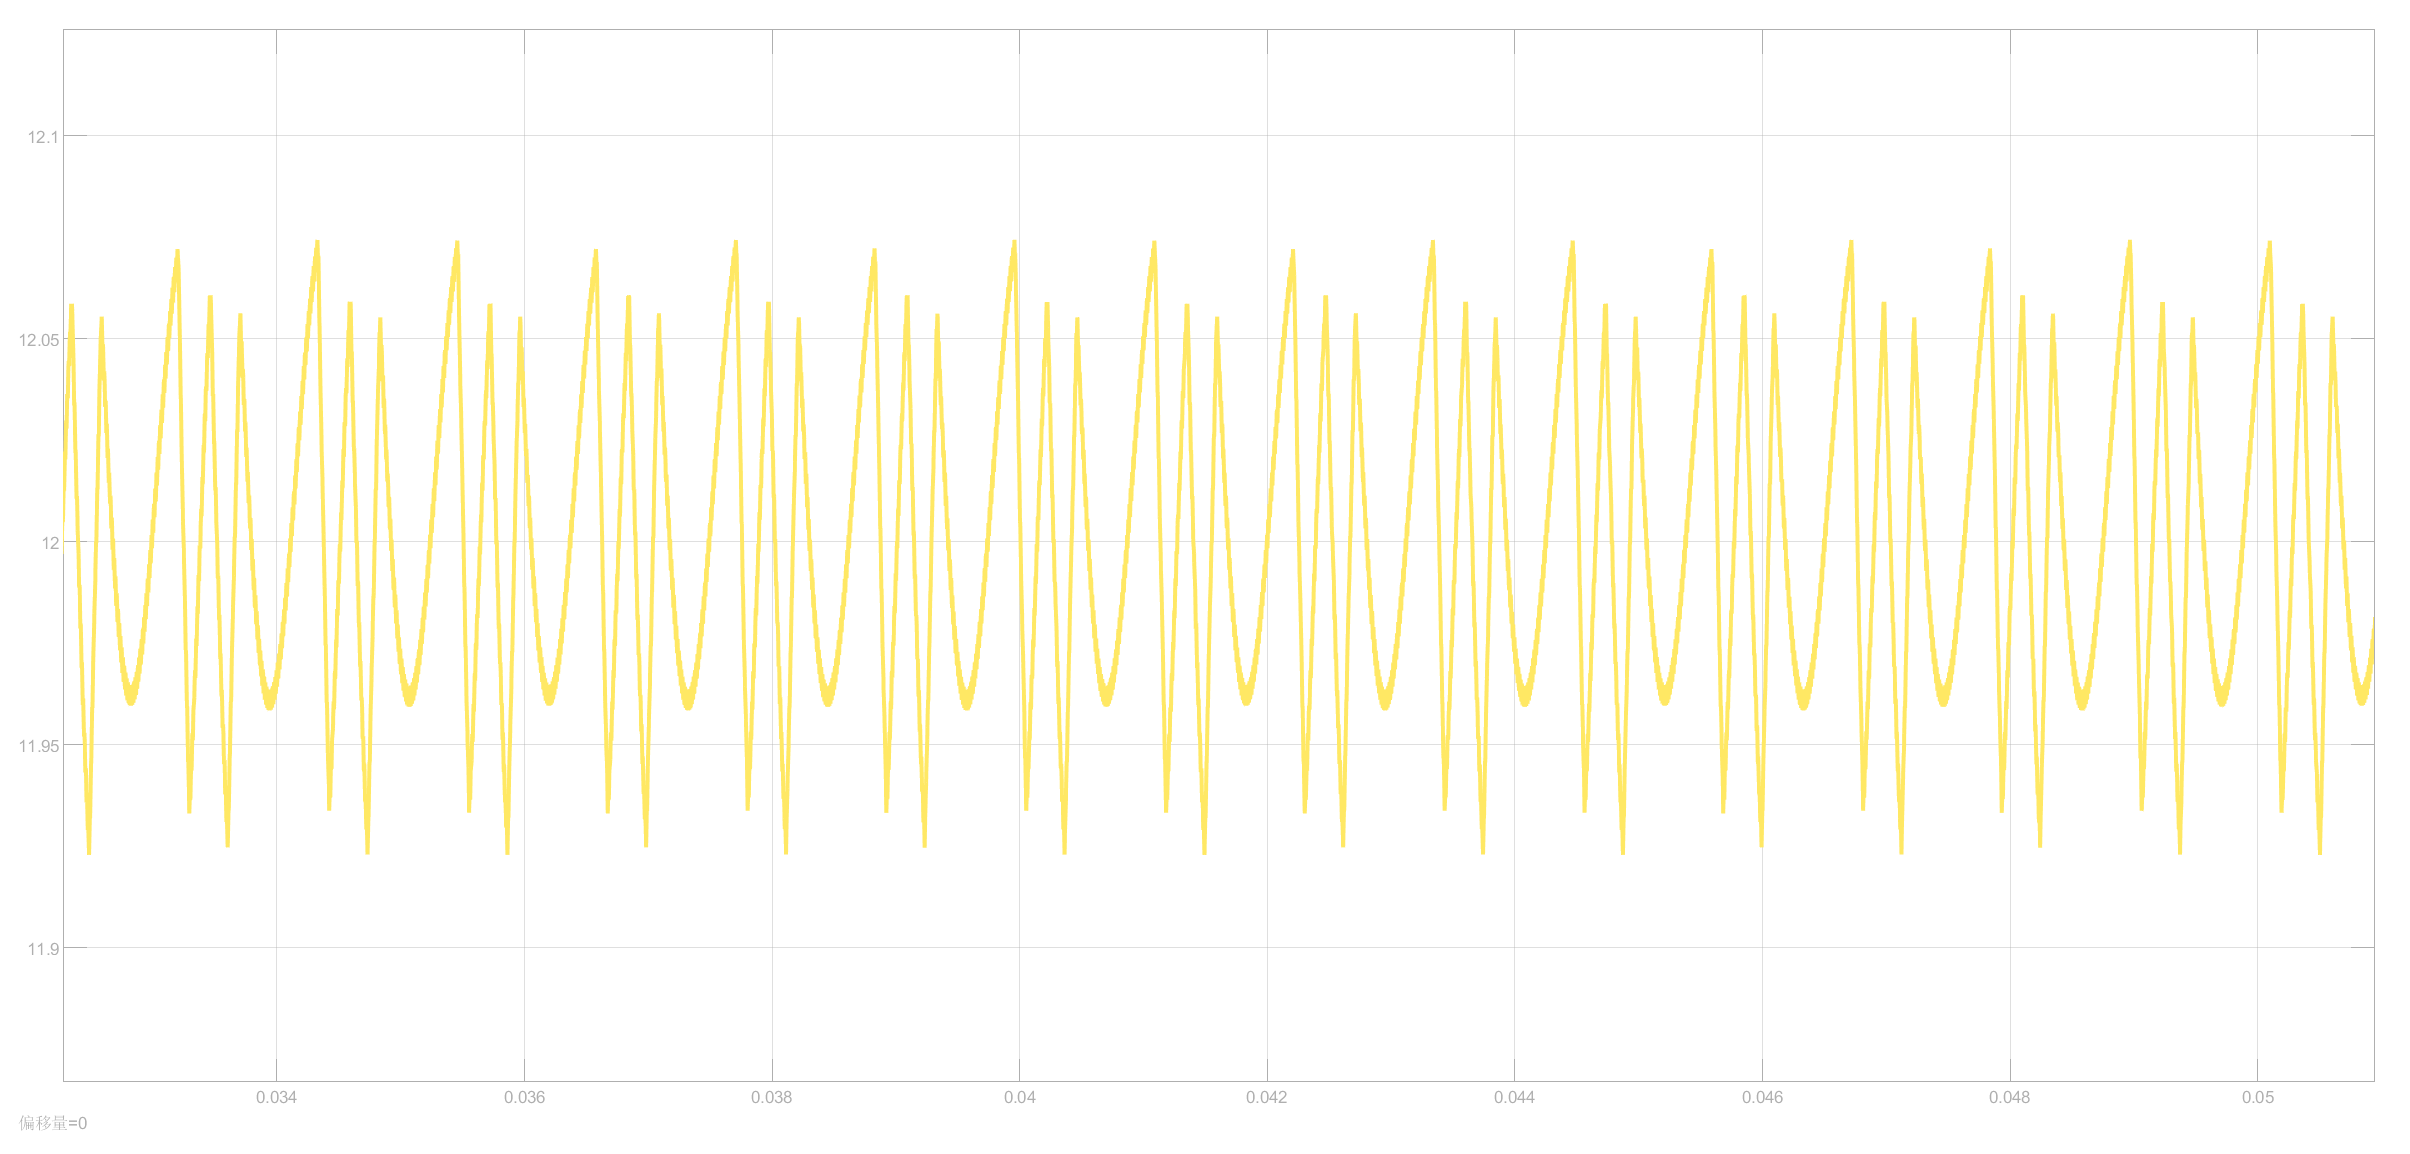
\includegraphics[width=0.8\textwidth]{image16.eps}
\caption{输出电压的纹波}
\end{figure}

由信号统计可知，输出电压纹波为$151.5mV$，双电平测量振幅为$36.36mV$。
\newpage
加入切载时，系统仿真结果如下：
\begin{figure}[htbp]
\centering  
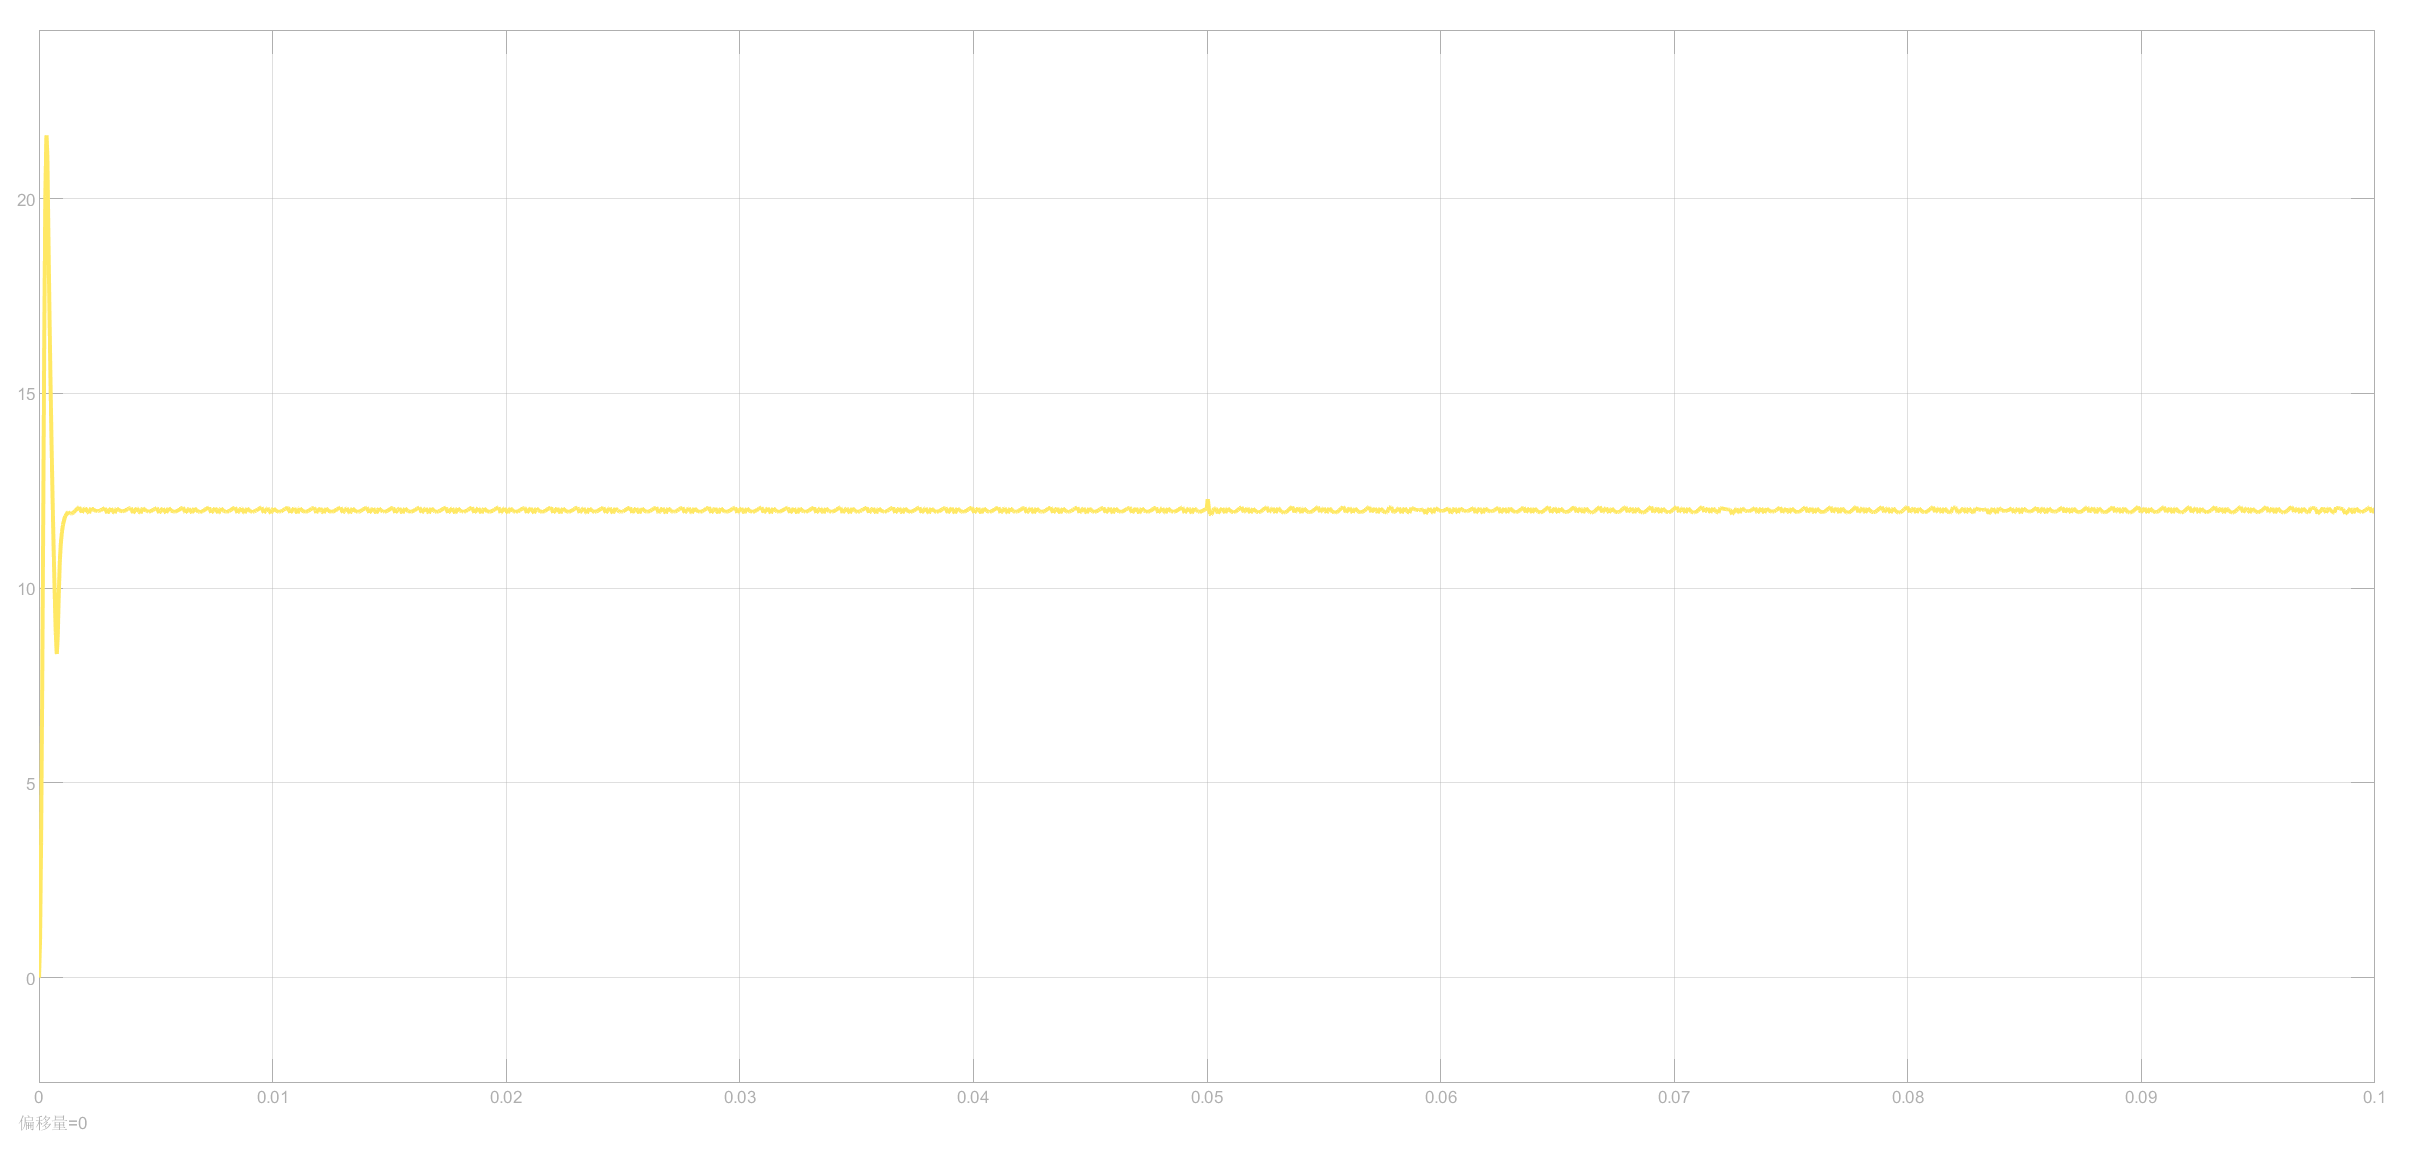
\includegraphics[width=0.8\textwidth]{image17.eps}
\caption{输入电压为42V，加入切载时，系统仿真结果}
\end{figure}

由信号统计可知，在$t=0.05s$处施加$10\%-100\%$的切载过程，输出电压超调量为$0.29V$，切载引起的电压跌落到$11.88V$,小于设计要求的$5\% \times 12V=0.6V$。

\textcircled{2}当输入电压为52V时

在稳态负载下仿真波形如下：
\begin{figure}[htbp]
\centering  
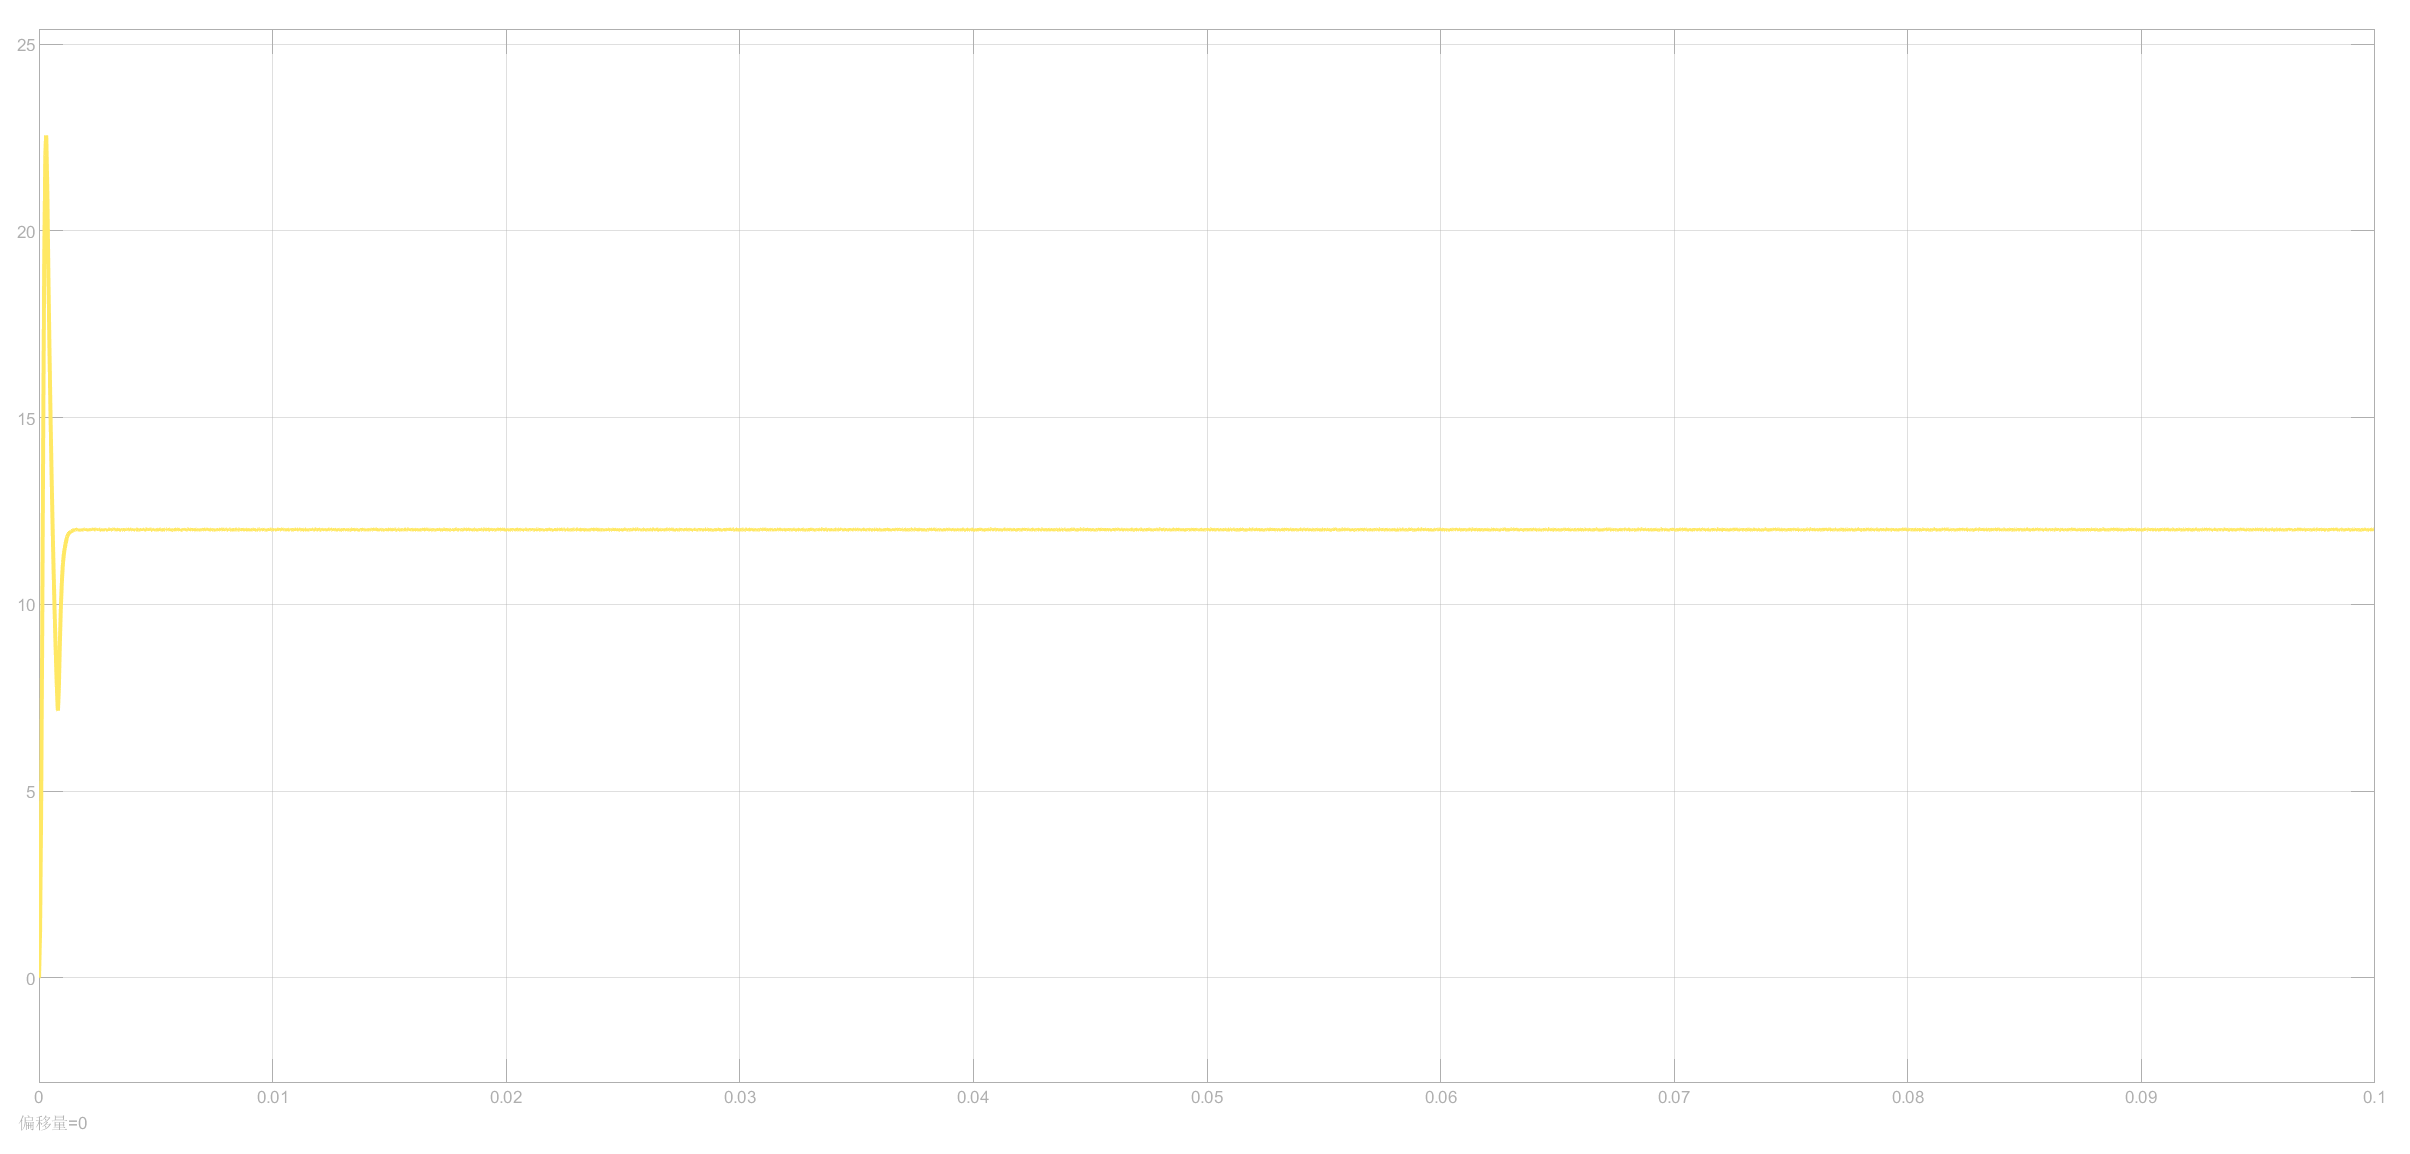
\includegraphics[width=0.8\textwidth]{image18.eps}
\caption{输入电压为52V，未加切载时，系统仿真结果}
\end{figure}
\newpage
单独观察电压纹波：
\begin{figure}[h]
\centering  
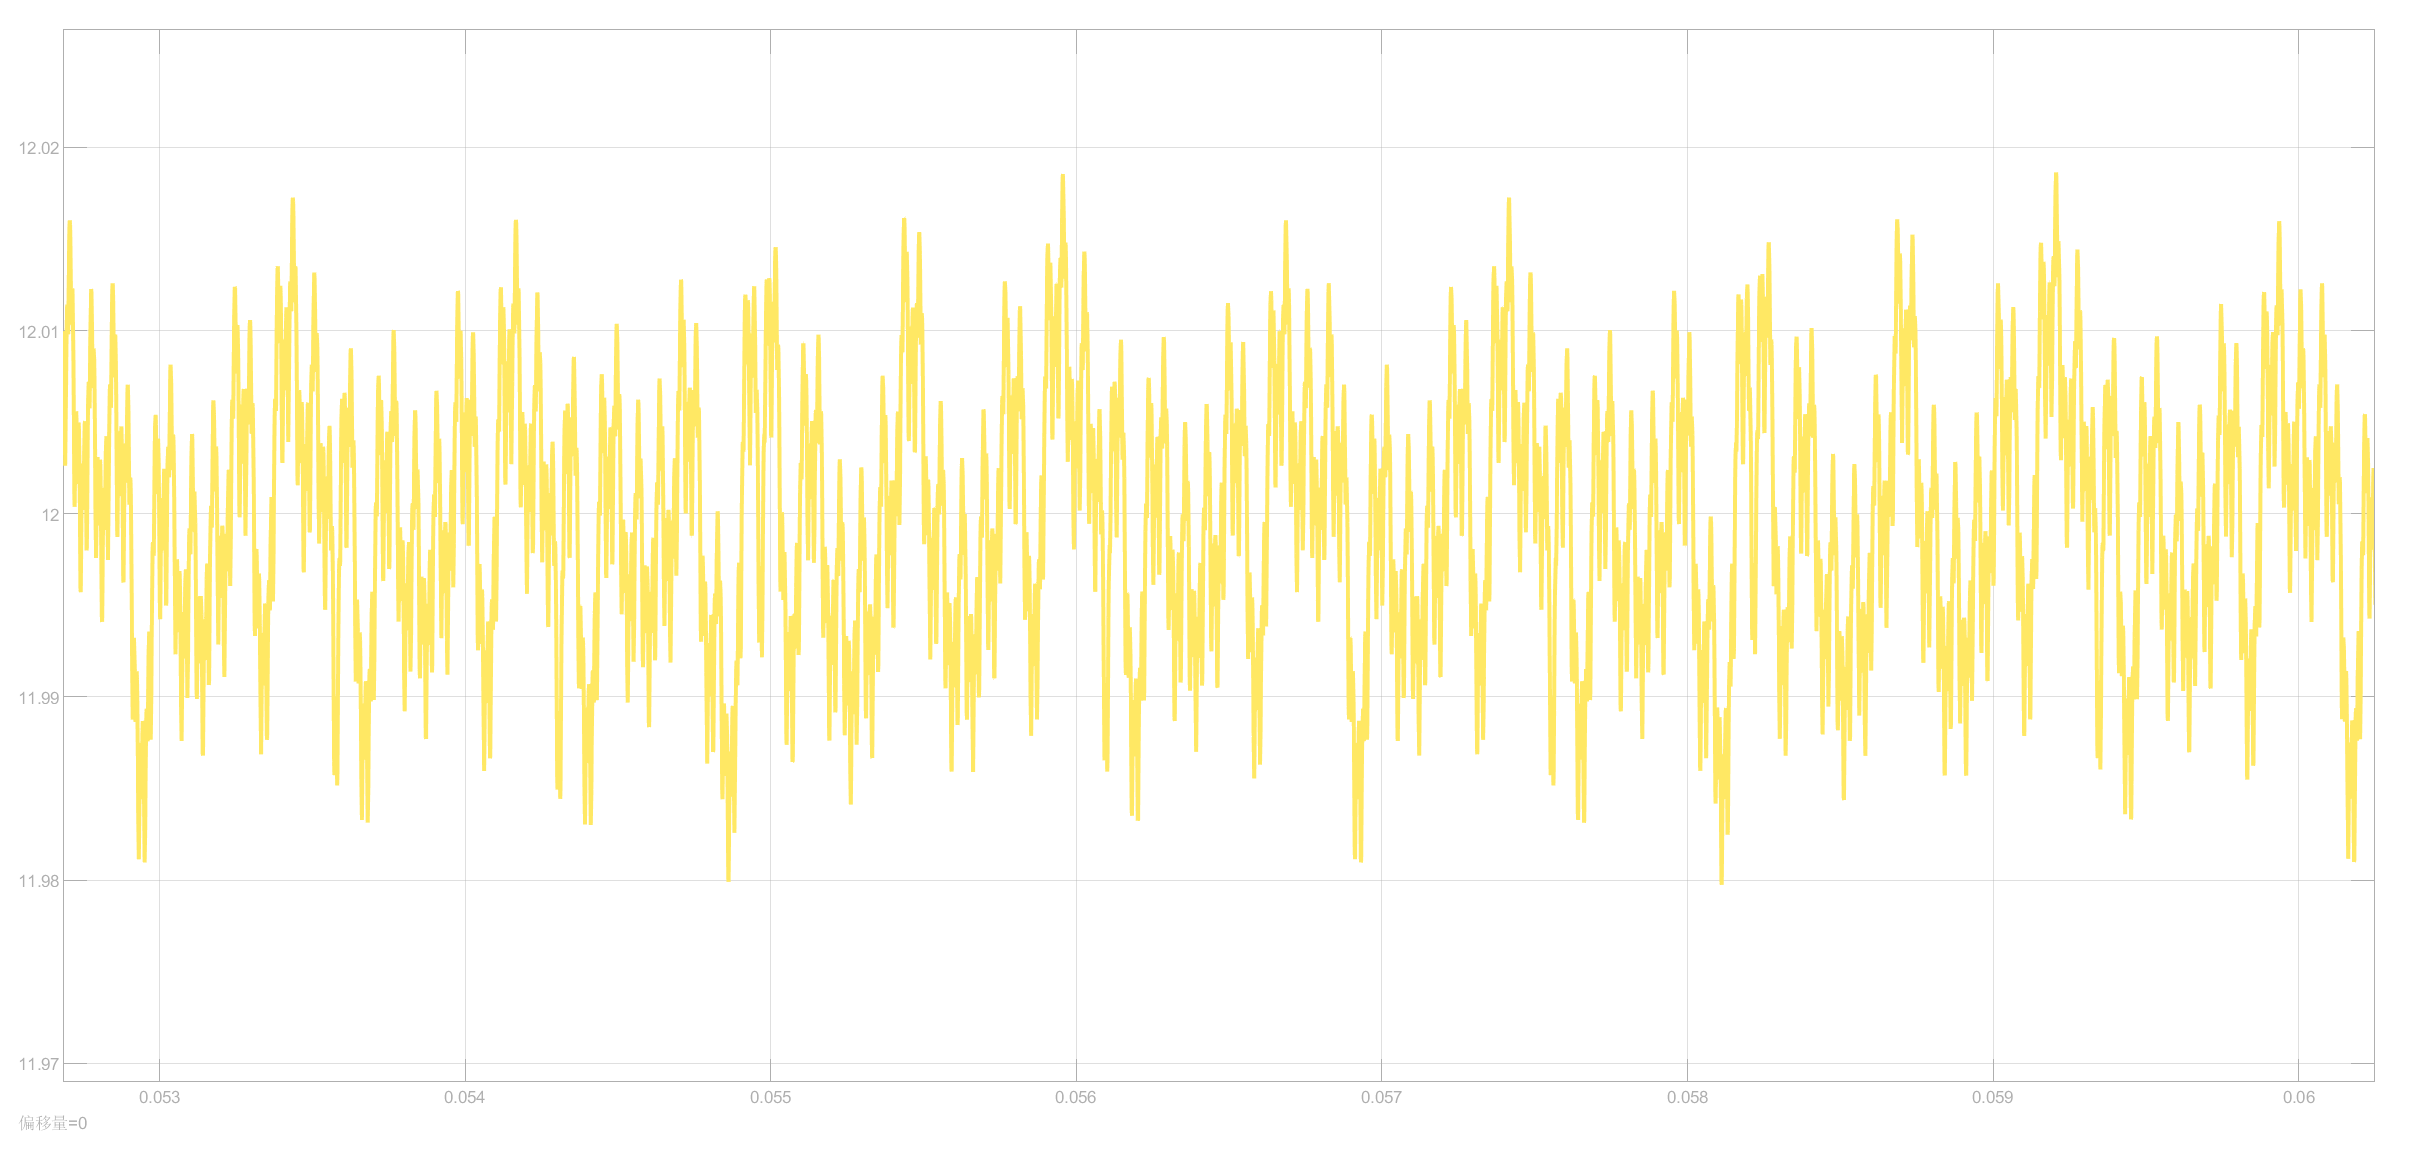
\includegraphics[width=0.8\textwidth]{image19.eps}
\caption{输出电压的纹波}
\end{figure}

由信号统计可知，输出电压纹波为$38.89mV$，双电平测量振幅为$1.945mV$。
\newpage
加入切载时，系统仿真结果如下：
\begin{figure}[htbp]
\centering  
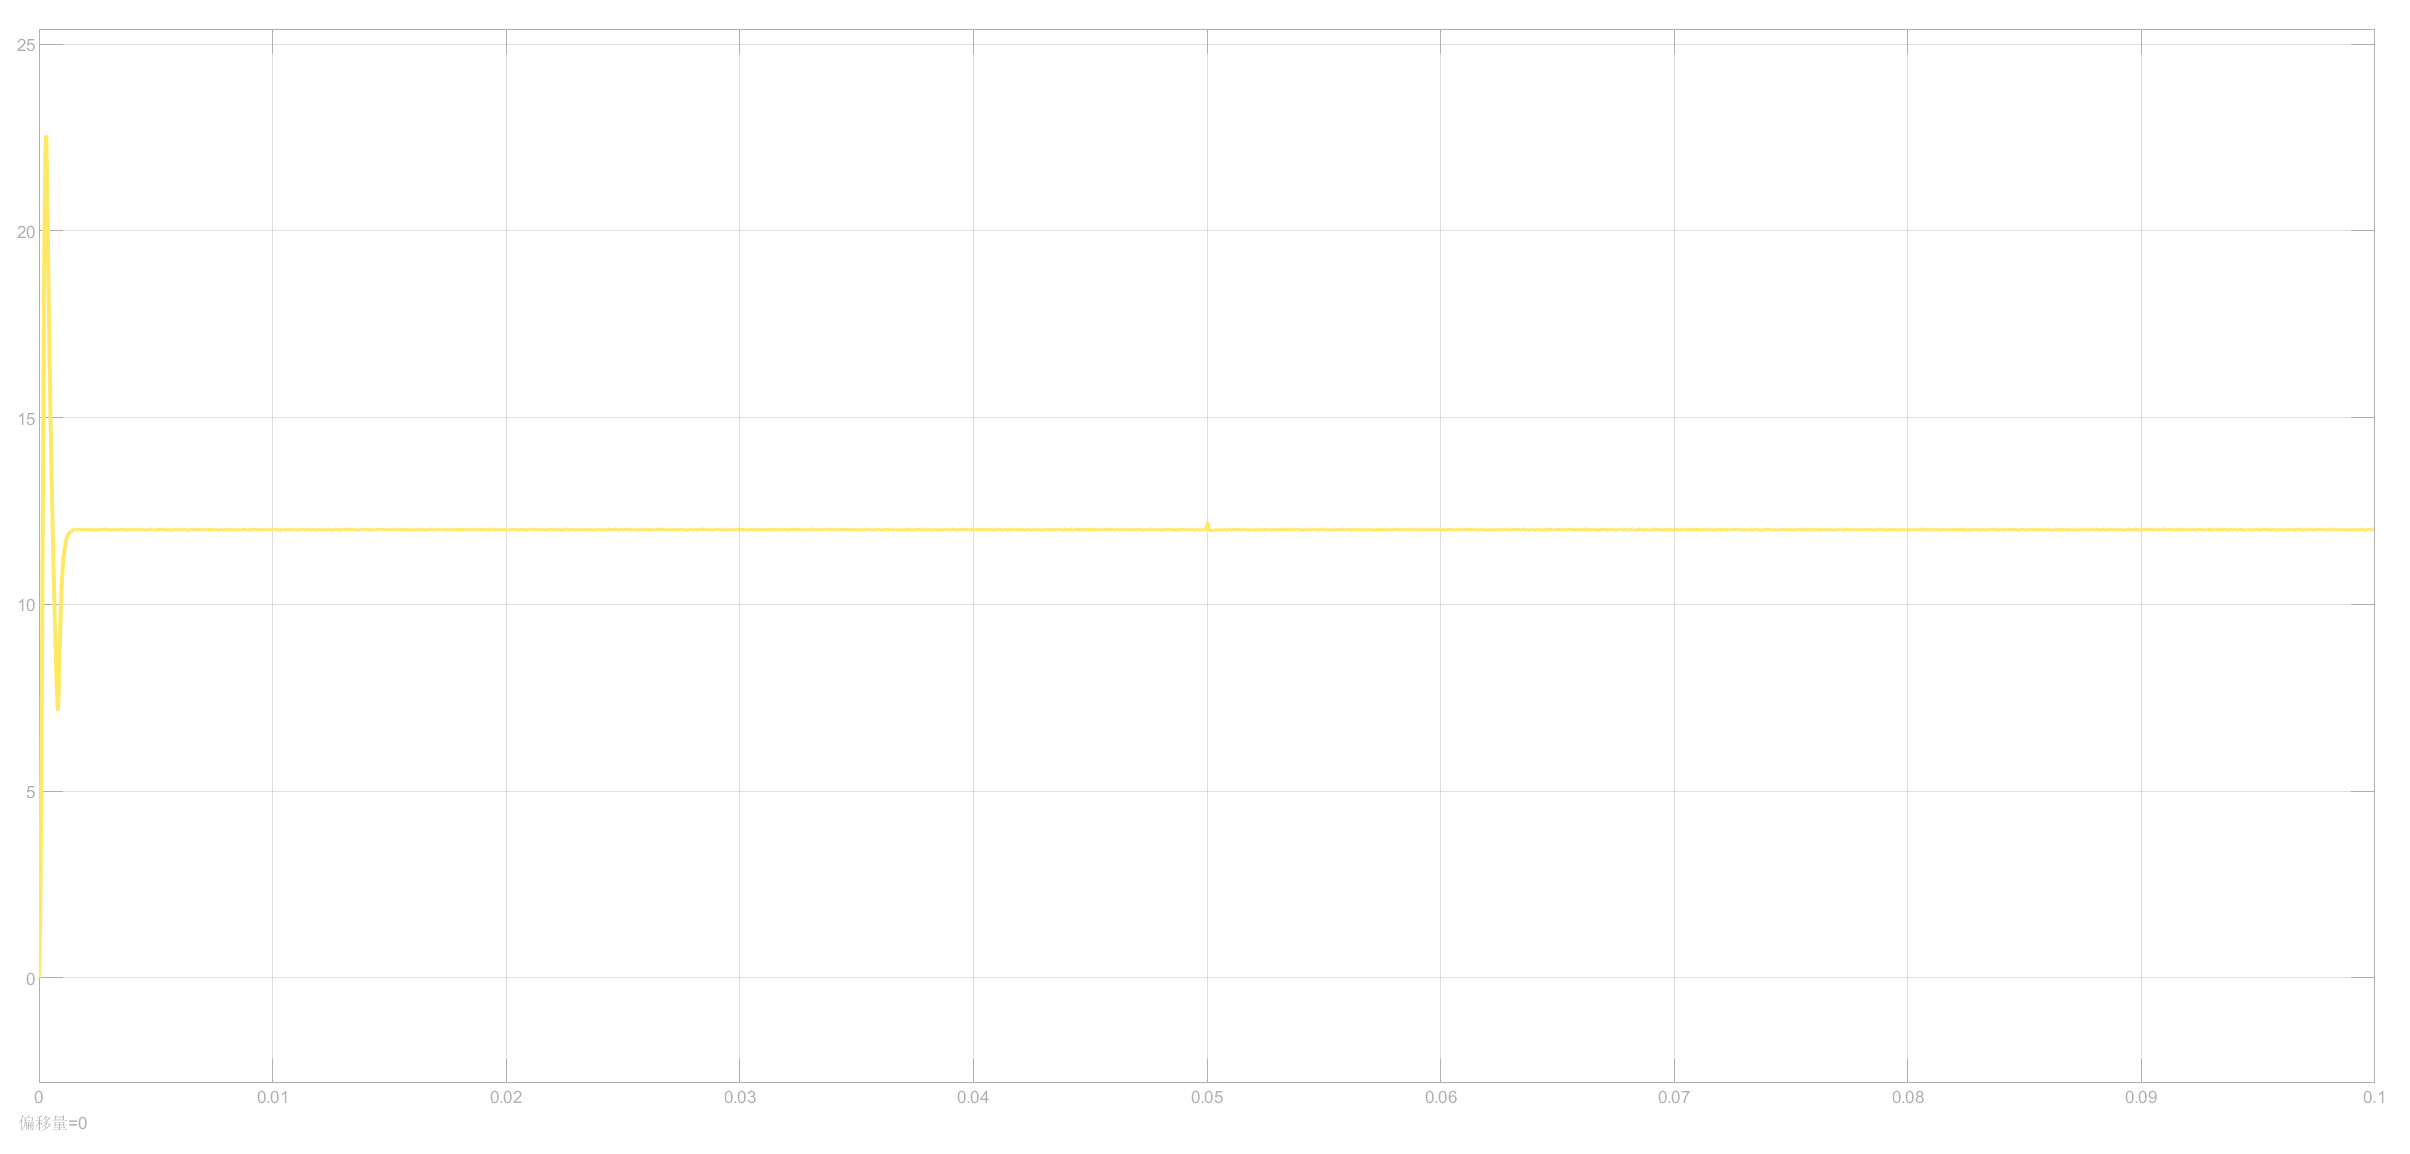
\includegraphics[width=0.8\textwidth]{image20.eps}
\caption{输入电压为52V，加入切载时，系统仿真结果}
\end{figure}

由信号统计可知，在$t=0.05s$处施加$10\%-100\%$的切载过程，输出电压超调量为$0.20V$，切载引起的电压跌落到$11.95V$,小于设计要求的$5\% \times 12V=0.6V$。

\textcircled{3}当输入电压为32V时

在稳态负载下仿真波形如下：
\begin{figure}[htbp]
\centering  
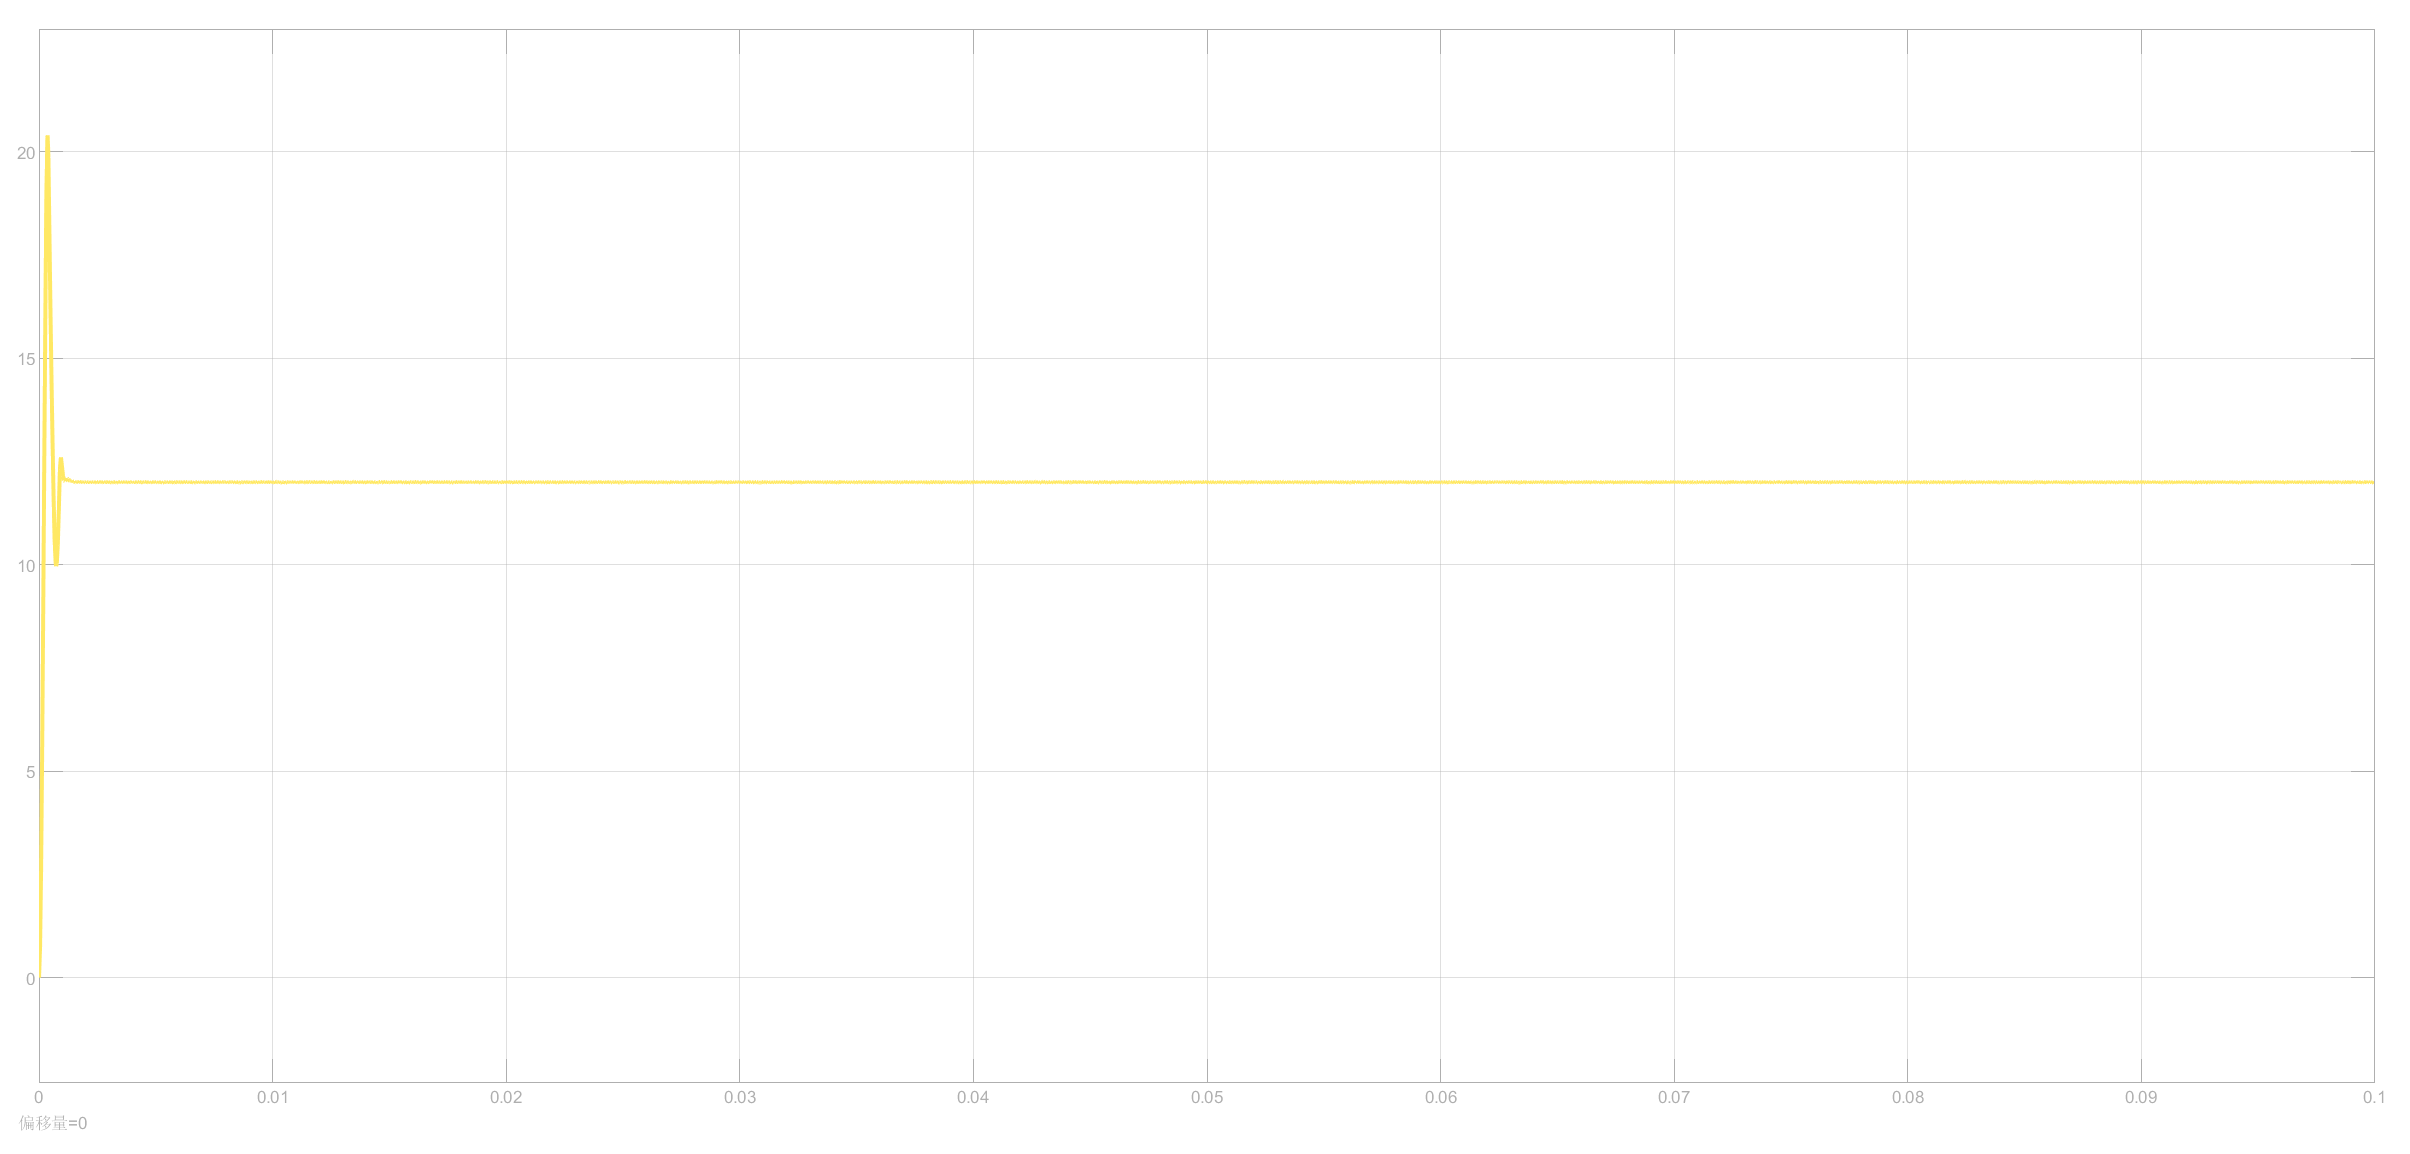
\includegraphics[width=0.8\textwidth]{image21.eps}
\caption{输入电压为32V，未加切载时，系统仿真结果}
\end{figure}
\newpage
单独观察电压纹波：
\begin{figure}[h]
\centering  
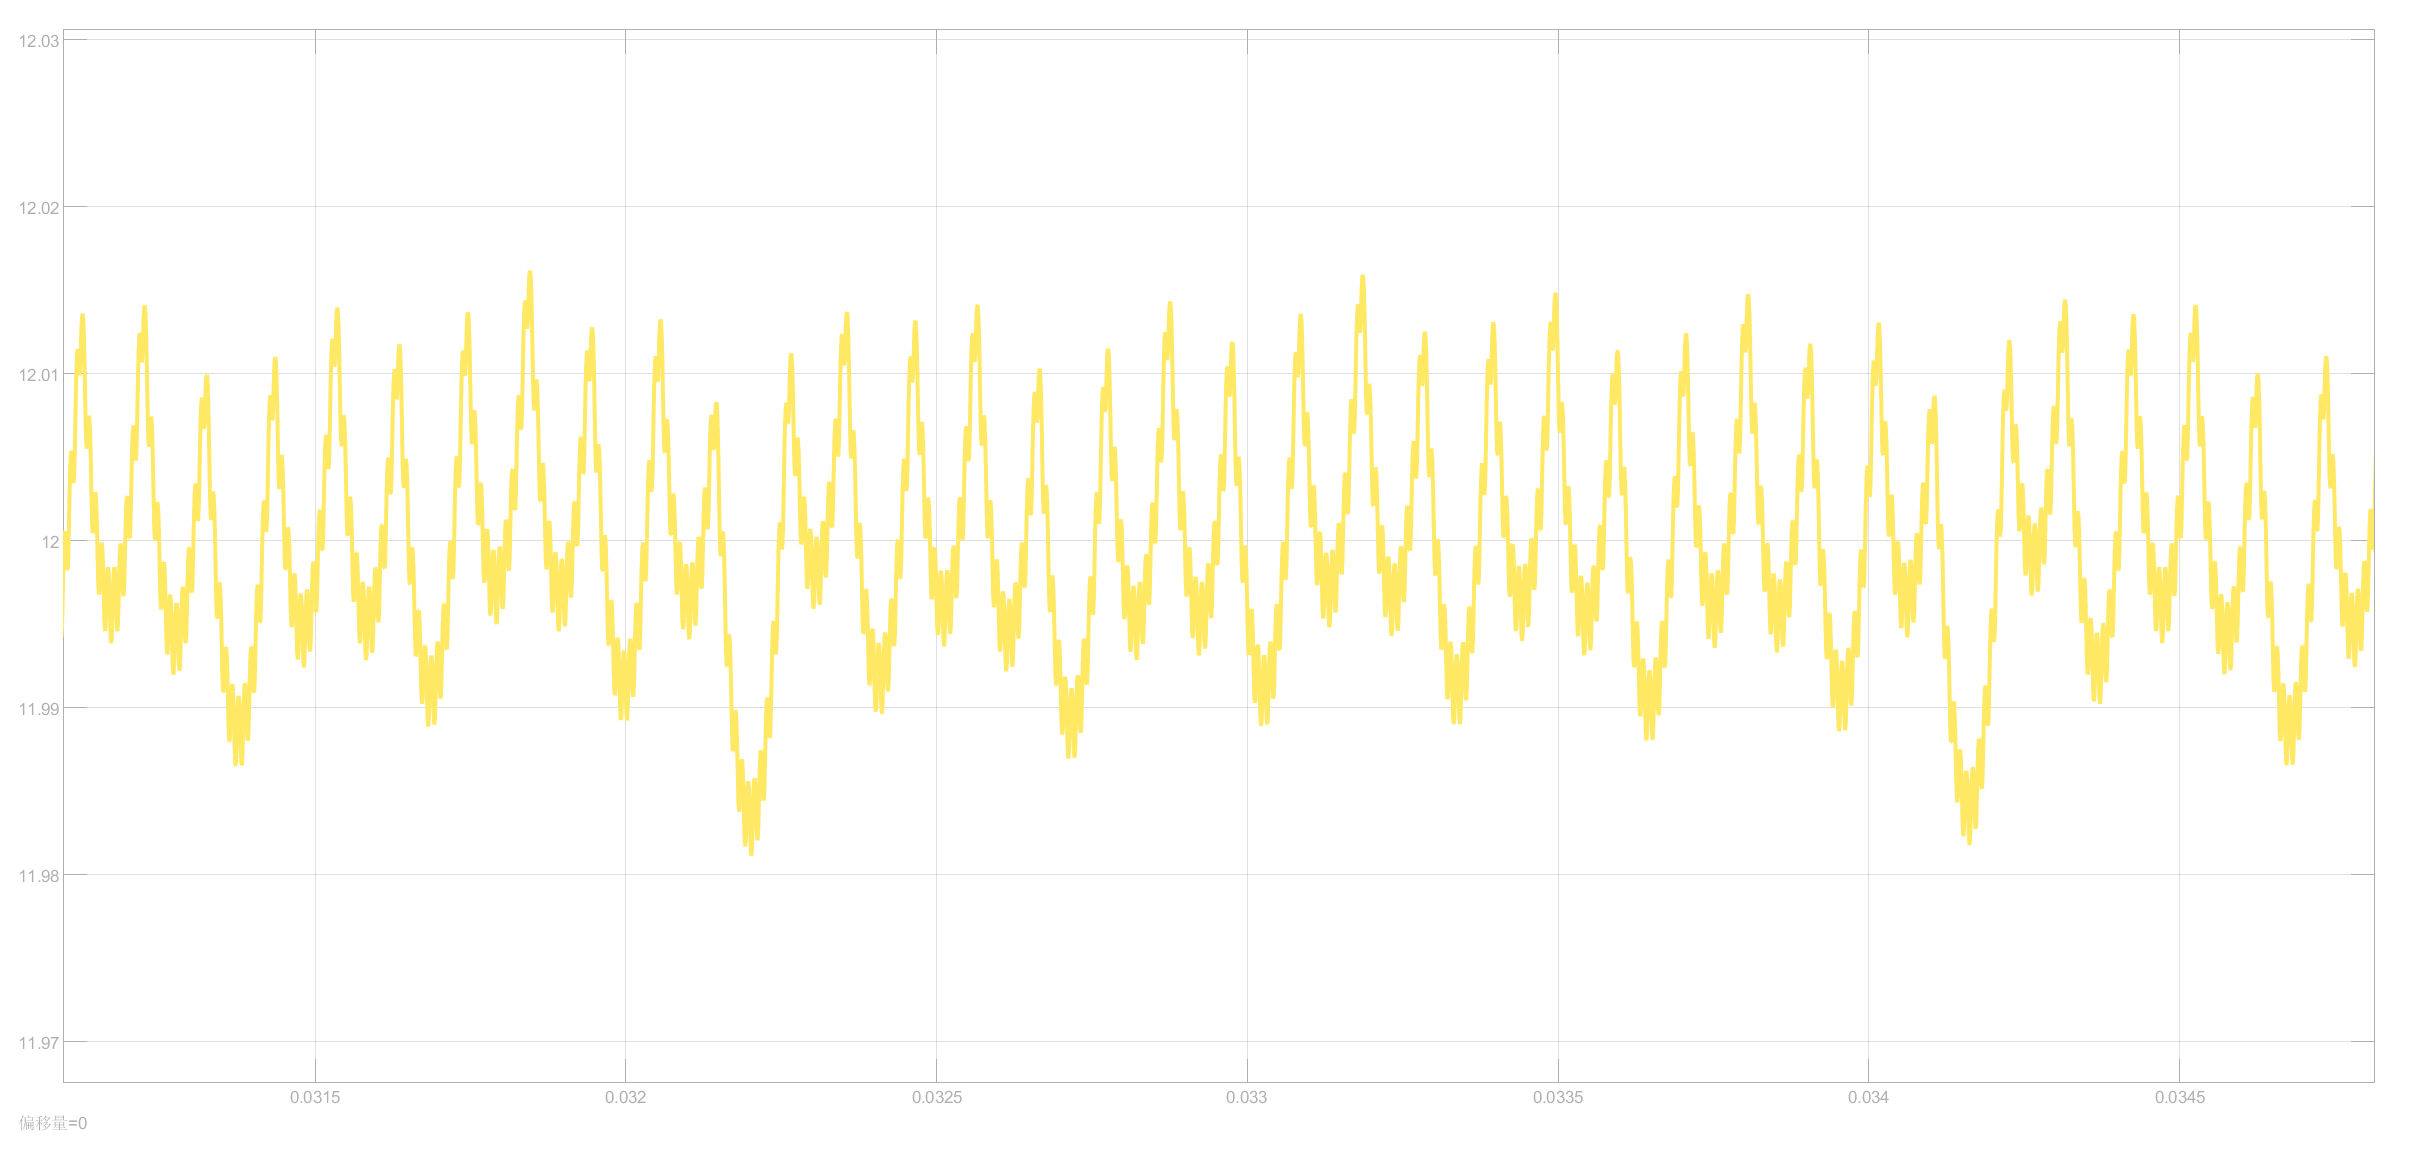
\includegraphics[width=0.8\textwidth]{image22.eps}
\caption{输出电压的纹波}
\end{figure}

由信号统计可知，输出电压纹波为$35.06mV$，双电平测量振幅为$1.052mV$。
\newpage
加入切载时，系统仿真结果如下：
\begin{figure}[htbp]
\centering  
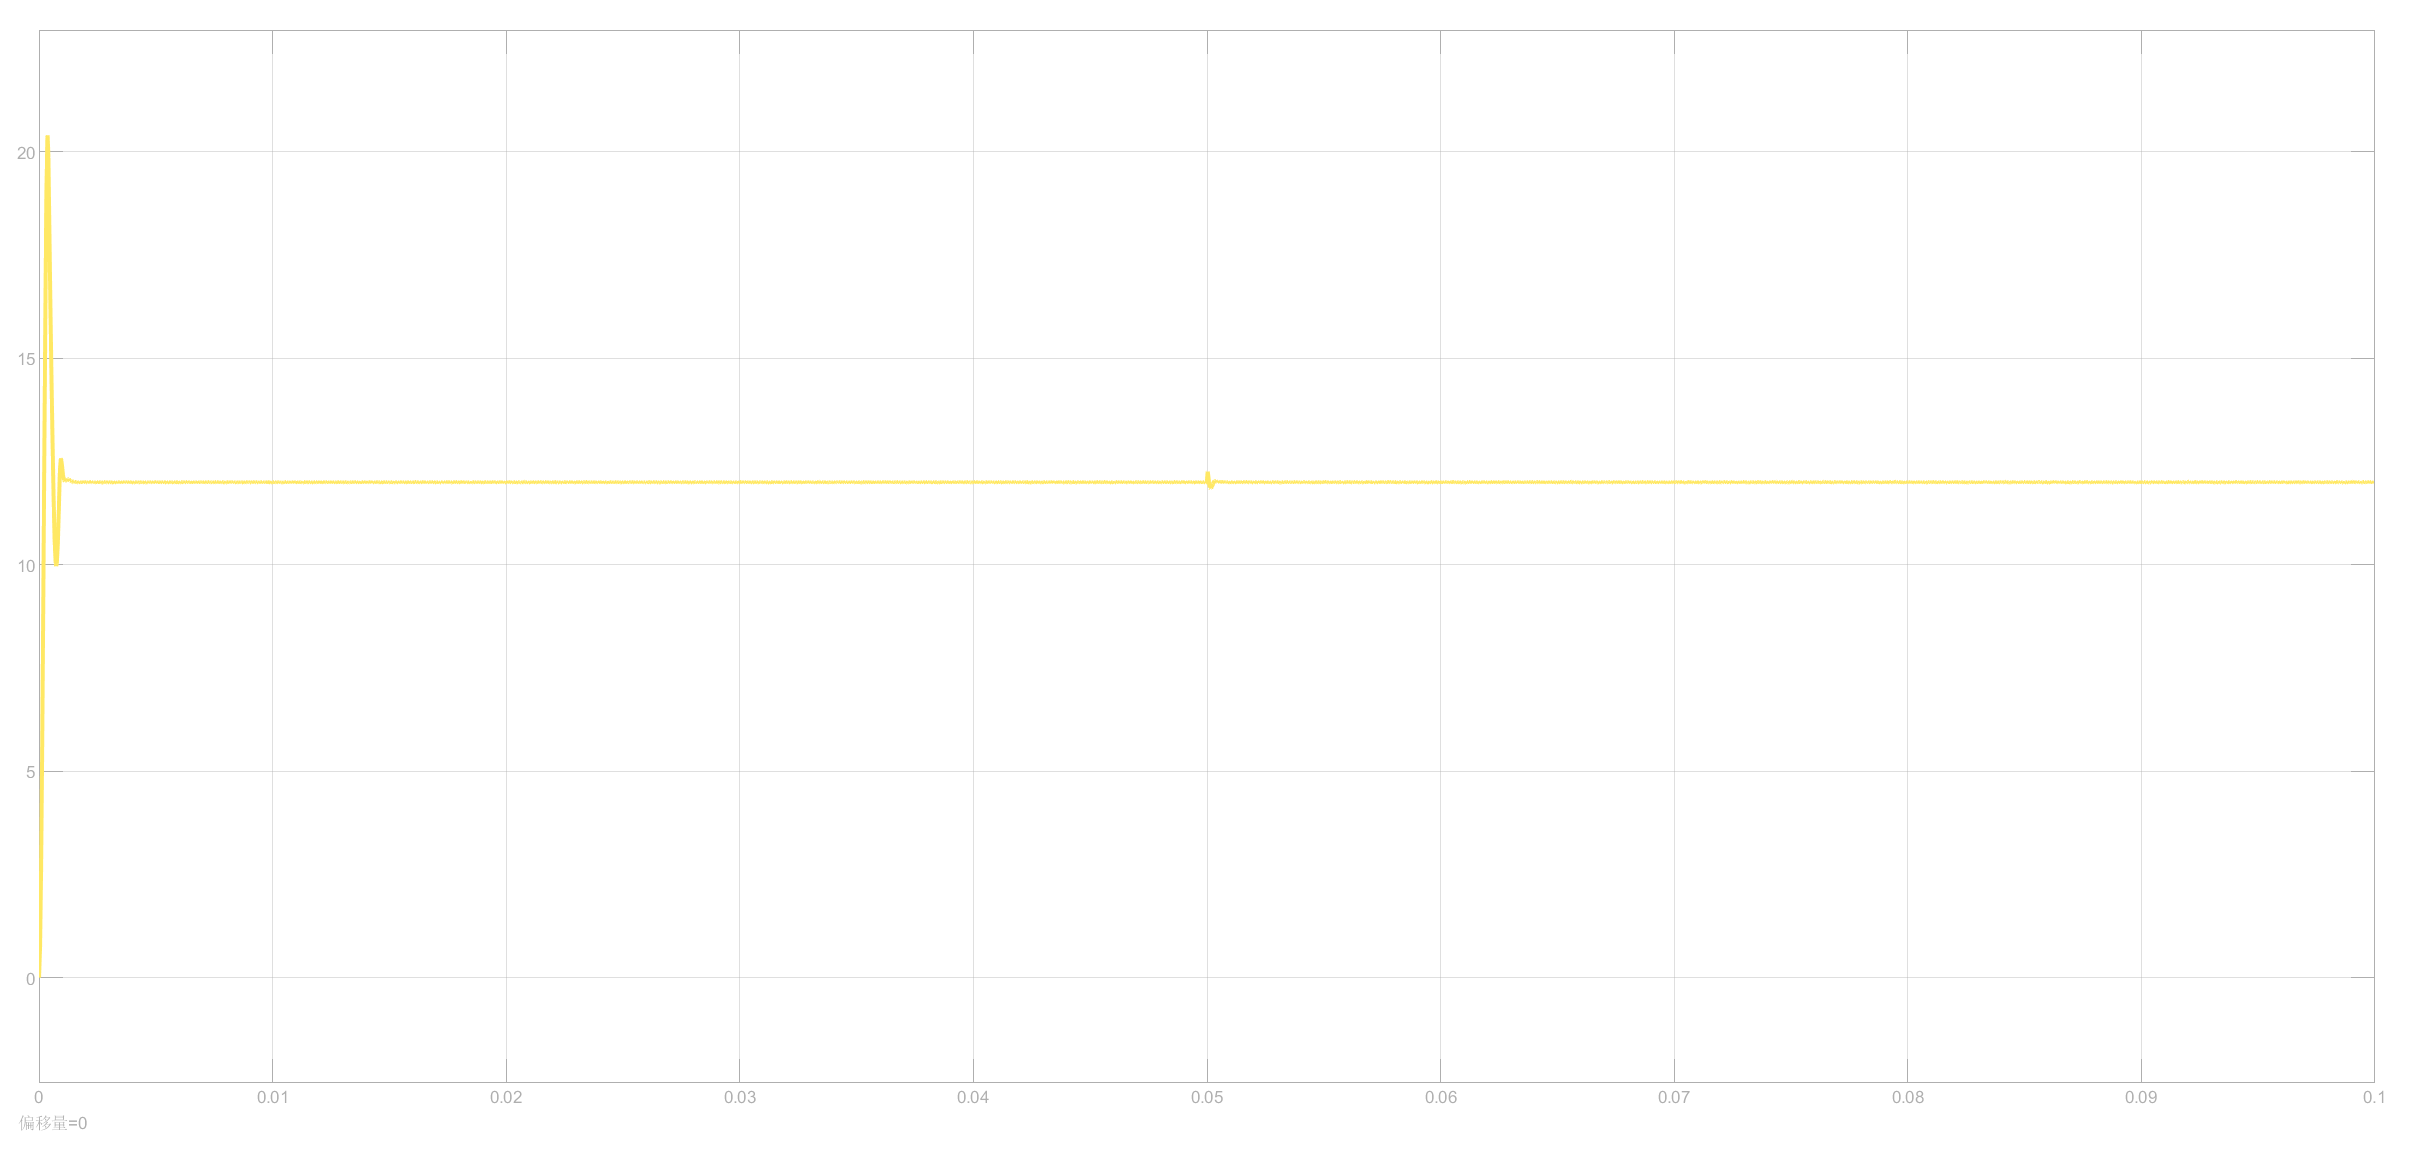
\includegraphics[width=0.8\textwidth]{image23.eps}
\caption{输入电压为32V，加入切载时，系统仿真结果}
\end{figure}

由信号统计可知，在$t=0.05s$处施加$10\%-100\%$的切载过程，输出电压超调量为$0.26V$，切载引起的电压跌落到$11.85V$,小于设计要求的$5\% \times 12V=0.6V$。

PID 控制器能够较好地控制 Buck 电路的输出电压，满足负载调整率$< 1\%$的设计要求，且在除了输出电压过大时纹波均能满足设计要求。
\section{总结}

本次 PID 和 fuzzy 的设计基本都能满足要求，PID 和 fuzzy 相比，fuzzy 调节时间明显小于 PID，
且在达到稳态时的超调量更小，说明 fuzzy 动态性能更优越；但是PID具有更小的过冲。
PID 和 fuzzy 在超调量、切载性能上都表现得比较好，设计都满足要求。
\end{document}
